\documentclass[twoside, 12pt]{report}

% --- PACCHETTI ---

% unità di misura e matematica
\usepackage{siunitx, amsmath}

% titolo capitoli e sezioni personalizzato
\usepackage{titlesec}

\titleformat{\chapter}
{\normalfont\LARGE\bfseries}{\thechapter.}{10pt}{\LARGE}
\titlespacing*{\chapter}{0pt}{0pt}{20pt}

\titleformat{\section}
{\normalfont\large\bfseries}{\thesection}{10pt}{\large}
\titlespacing*{\section}{0pt}{0pt}{10pt}

% include pdfs
\usepackage{pdfpages}

% grafiche e tabelle
\usepackage{graphicx, calc}

\graphicspath{{images/}}

\usepackage{tikz, pgfplots, pgfplotstable}

\pgfplotsset{compat = newest}
\usepgfplotslibrary{units}

\usepackage{array, csvsimple}

\newcolumntype{C}{>{\centering}m{1.8cm}}
\newcolumntype{L}{>{\centering\arraybackslash}m{1.8cm}}
\newcolumntype{I}{>{\centering}m{2.5cm}}
\newcolumntype{U}{>{\centering\arraybackslash}m{2.5cm}}

\usepackage{float}

% colori personalizzati
\usepackage{colortbl, xcolor}

% normali
\definecolor{myBlue}{RGB}{1, 187, 235}
\definecolor{myRed}{RGB}{255, 43, 43}
\definecolor{myYellow}{RGB}{255, 221, 86}
\definecolor{myBlack}{RGB}{28, 28, 28}
\definecolor{myGrey}{RGB}{134, 134, 134}
% chiari
\definecolor{myLightBlue}{RGB}{177, 239, 255}
\definecolor{myLightRed}{RGB}{255, 177, 177}
\definecolor{myLightYellow}{RGB}{255, 240, 180}
\definecolor{myLightGrey}{RGB}{218, 218, 218}

\pgfplotscreateplotcyclelist{modular}{
        {myBlue},
        {myRed},
        {myBlack},
        {myGrey},
        {myYellow},
      }

\usepackage{subcaption, caption}

% numerazione capitoli in italiano
\usepackage[italian]{babel}

% spaziatura
\usepackage{parskip}

% impaginazione
\usepackage{setspace} % For doublespacing

\doublespacing

\usepackage{geometry}

\geometry{a4paper, top = 2cm, bottom = 2cm, outer = 2cm, inner = 3cm, heightrounded}

% font
\usepackage{times}

% bibliografia
\usepackage{csquotes, biblatex}
\addbibresource{bibliography.bib}

\usepackage{xurl, url} % evita che la bibliografia esca dal margine

\urlstyle{same}
\appto{\bibsetup}{\raggedright}

% salta pagine bianche
\usepackage{afterpage}

\newcommand\emptypage{
    \newpage
    \thispagestyle{empty}
    \mbox{}
    \newpage
}

% interlinea
\linespread{1.5}

% comandi per aggiungere chapter, section e subsection non numerate al toc
\newcommand\unchapter[1]{
    \chapter*{#1}
    \addcontentsline{toc}{chapter}{#1}}

\newcommand\unsection[1]{
    \section*{#1}
    \addcontentsline{toc}{section}{#1}}

\newcommand\unsubsection[1]{
        \subsection*{#1}
        \addcontentsline{toc}{subsection}{#1}}

% --- DOCUMENTO PRINCIPALE ---

% inizio del documento
\begin{document}

% --- FRONTESPIZIO ---
% DA MODIFICARE DATA DI LAUREA !!!

\includepdf{pdfs/frontespizio/frontespizio_tesi.pdf}
\emptypage

% --- INDICE ---

\tableofcontents
\emptypage

% --- CAPITOLI ---

\unchapter{Introduzione e Specifiche di Progetto}

%--------------------------------------------------------------------------------------------

In questa tesi viene discussa la progettazione di un sintetizzatore musicale compatibile con
lo standard modulare più diffuso al giorno d'oggi, ovvero Eurorack \cite{eurorack}. Più
precisamente si vuole realizzare un generatore di segnali che offra la possibilità di essere
controllato in tensione (Voltage Controlled Oscillator, o VCO in breve). In questo modo,
applicando dei segnali variabili nel tempo in ingresso al modulo, si è in grado di variare
dinamicamente la frequenza dei segnali in uscita.

Il range scelto per tale variazione comprende la fascia di frequenze utili nello spettro
audio, quindi da poche decine di $Hz$ a circa $7kHz$. Si desidera inoltre, la possibilità di
convertire a piacere il funzionamento del modulo in oscillatore a bassa frequenza (Low Frequency
Oscillator, o LFO), spostando quindi il range di frequenze disponibili da frazioni di
$Hz$ a qualche decina di $Hz$.
\medskip

\begin{figure}[ht]
    \centering
    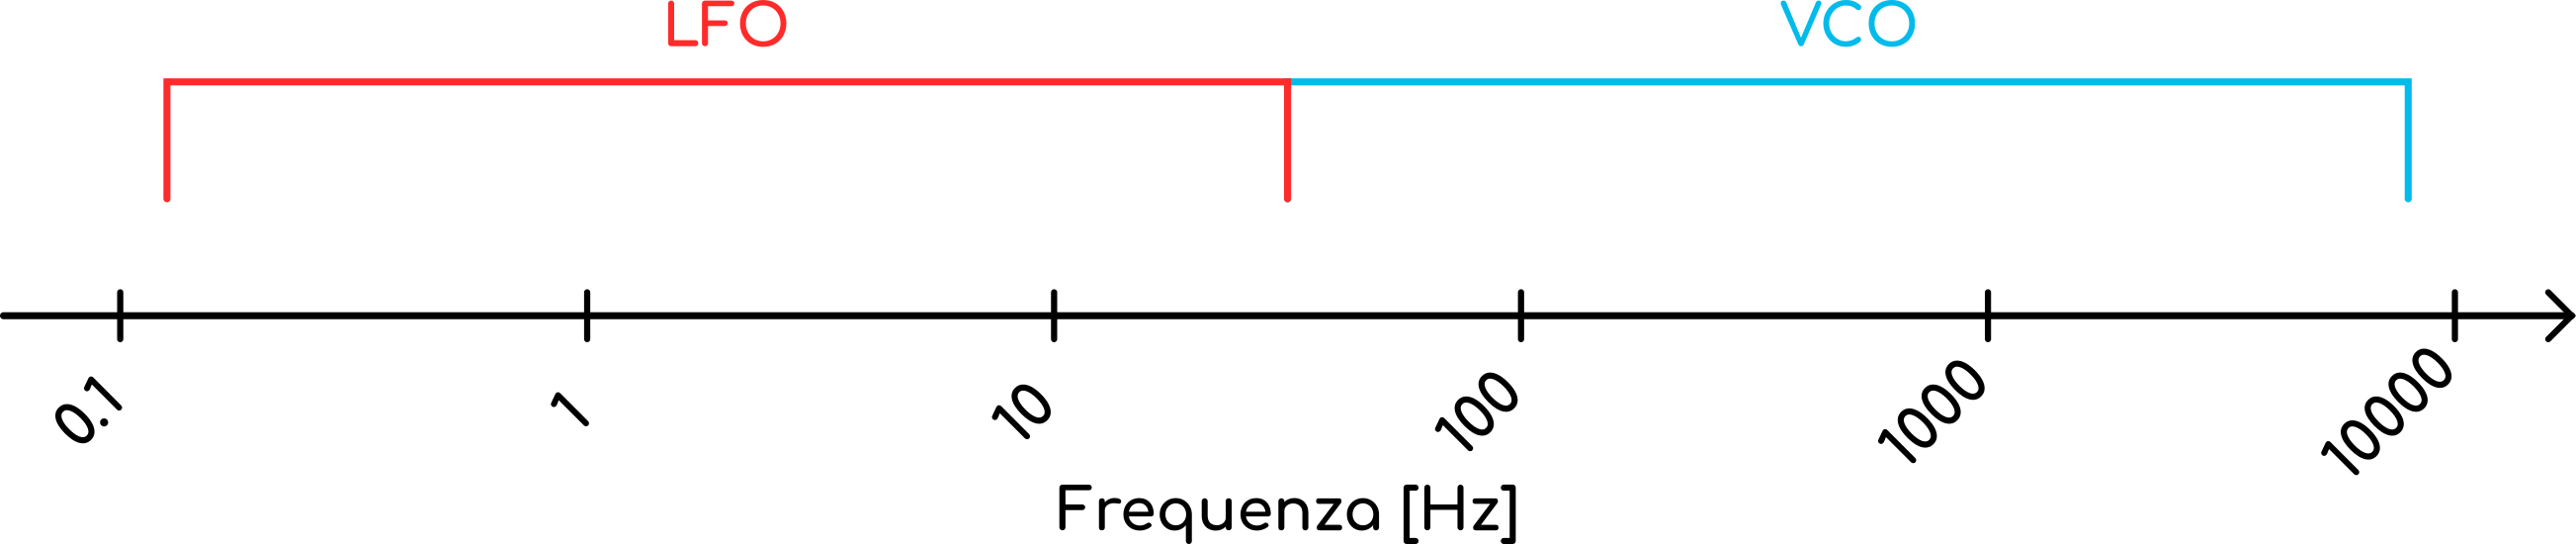
\includegraphics{graphs/functioning_range.png}
    \caption{Range di funzionamento in scala logaritmica}
    \label{functioning_range}
\end{figure}

In modalità VCO quindi, il modulo produrrà dei segnali che attraverso un adeguato sistema
potranno essere ascoltati, mentre in modalità LFO il circuito produrrà dei segnali lentamente
variabili nel tempo, utili per la modulazione e il controllo di parametri in altri moduli
eventualmente presenti nel sistema.

Le forme d'onda desiderate sono quelle base, ovvero:

\begin{itemize}
    \item Sinusoide;
    \item Onda Quadra;
    \item Triangolo;
    \item Rampa;
    \item Dente di sega (sebbene nel range VCO non risulti particolarmente differente dalla
          rampa in termini di suono, per quanto riguarda il funzionamento LFO la differenza
          è radicale, poichè il segnale viene solitamente utilizzato come modulante);
\end{itemize}

inoltre, come verrà illustrato più avanti, risulta piuttosto semplice anche estrarre un
segnale a impulso, rigorosamente alla stessa frequenza di quelli già generati. Tale segnale
può essere utilizzato per scopi simili a quelli dei segnali in uscita in modalità LFO.
\smallskip

Per quanto riguarda le specifiche sui livelli di tensione, si vogliono imporre i seguenti
intervalli di valori:

\begin{itemize}
    \item Segnali audio (i 5 elencati poco sopra): $\pm5V$;
    \item Segnali logici (impulso): $(0V,5V)$;
    \item Tensione di ingresso: $(0V,8V)$ in modalità $1V/Octave$, ovvero facendo in modo che
          ad un incremento di $1V$ corrisponda un raddoppio di frequenza, cioè un'ottava;
    \item Alimentazioni: $\pm12V$ e $+5V$;
\end{itemize}

Le specifiche sopra riportate sono prese dallo standard Eurorack.

Altre caratteristiche volute sono:

\begin{itemize}
    \item Manopole per il controllo del "volume" di segnali in ingresso e uscita, ad eccezione
          dell'impulso;
    \item Manopole per il controllo manuale della frequenza;
\end{itemize}

Raccogliendo tutti questi dettagli possiamo iniziare a pensare ad una interfaccia utente,
riportata in figura \ref{panel_explained}, in modo da rendere più chiaro al lettore il
prodotto finale.
\medskip

\begin{figure}[ht]
    \centering
    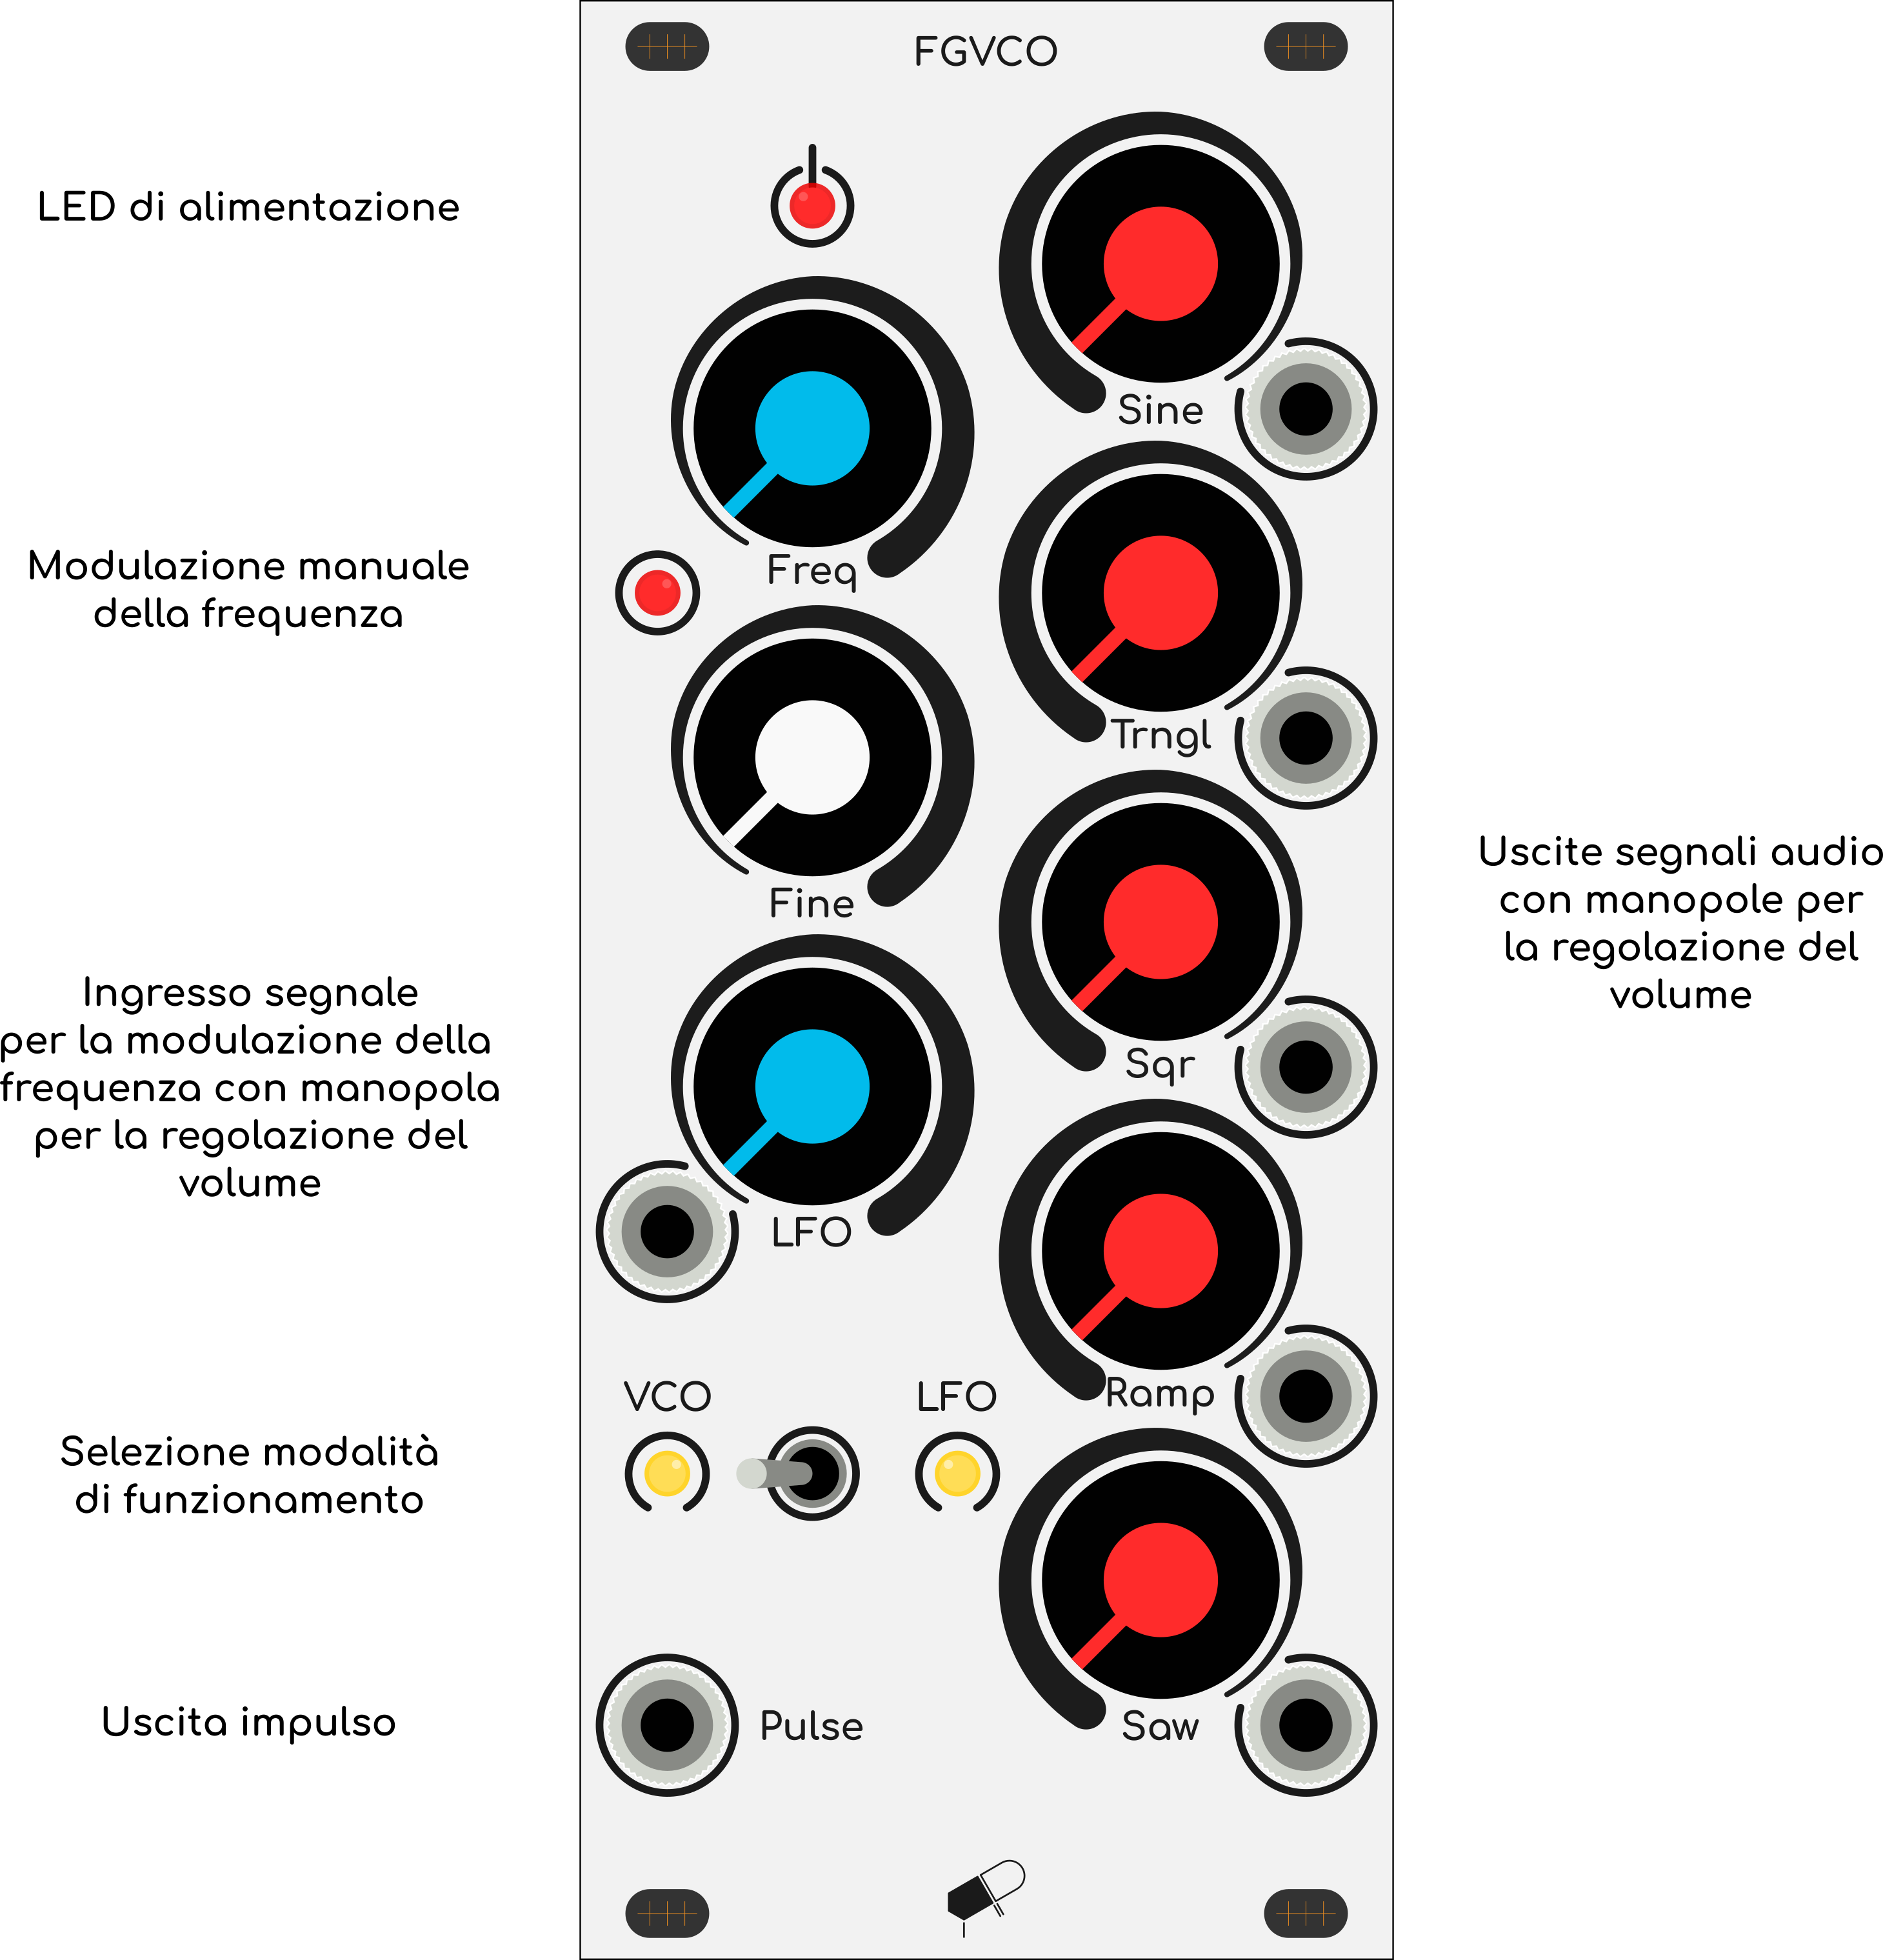
\includegraphics{misc/panel_explained.png}
    \caption{Pannello frontale del modulo}
    \label{panel_explained}
\end{figure}

Si decide di realizzare l'intero circuito senza l'utilizzo di microcontrollori o sistemi
programmabili. Tale scelta viene presa per mettere alla prova più competenze possibili tra
quelle acquisite durante gli anni di studio. Si potrebbe infatti realizzare il tutto con un
microcontrollore dotato di forme d'onda densamente campionate salvate in memoria.
Altro motivo per il quale si sceglie questa strada è per avere ogni segnale su un canale
a sè in modo da poter usufruire di ognuno contemporaneamente.

%--------------------------------------------------------------------------------------------

\chapter{Generazione dei Segnali Principali}

%--------------------------------------------------------------------------------------------

Per la generazione dei segnali a rampa e a triangolo si decide di procedere in ogni caso
per via digitale, utilizzando dei contatori binari abbinati ad un convertitore
digitale-analogico.

%--------------------------------------------------------------------------------------------

\section{Rampa}

%--------------------------------------------------------------------------------------------

\subsection*{Principio di Funzionamento}

%--------------------------------------------------------------------------------------------

Per il segnale a rampa si fa uso di un contatore unidirezionale, ovvero un dispositivo
in grado di contare automaticamente da $0$ a $2^n$ (con $n$ numero di bit) semplicemente
fornendo un segnale di clock adeguatamente dimensionato. Maggiore il numero di bit,
maggiore la precisione del nostro segnale, quindi minore l'intensità del rumore generato.

\begin{figure}[H]
    \centering

    \begin{subfigure}{.5\textwidth}
        \centering
        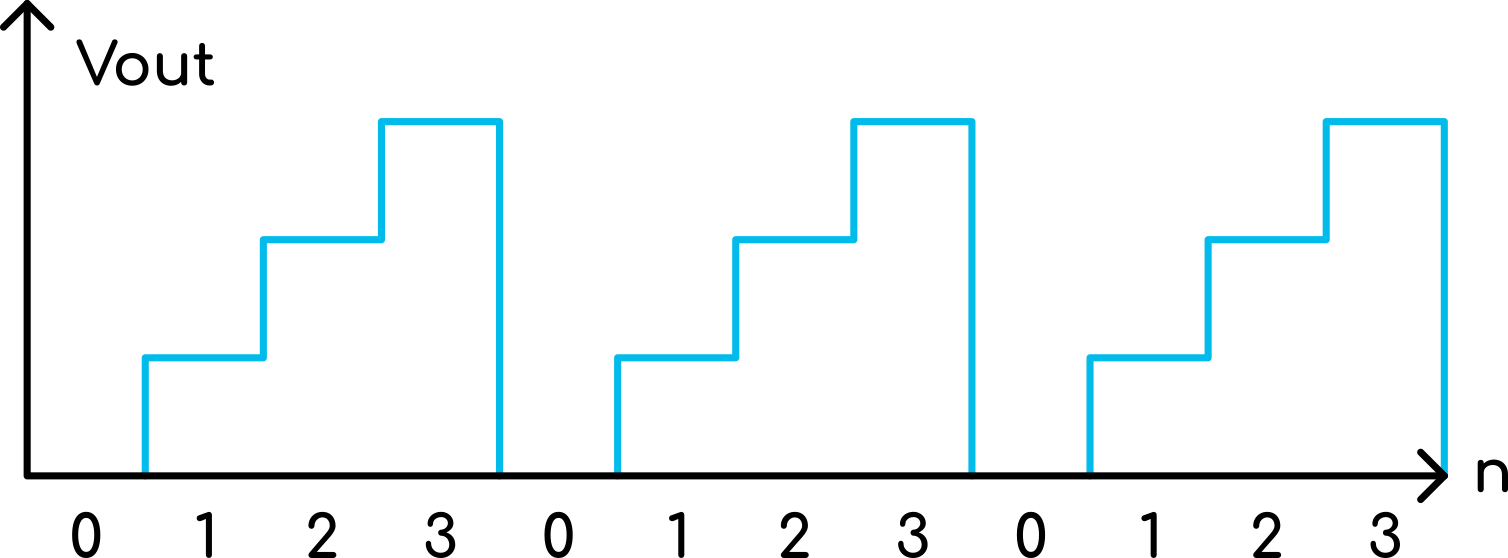
\includegraphics{graphs/low_res_ramp.png}
        \caption{Rampa ottenuta con un contatore a 2 bit}
        \label{low_res_ramp}
    \end{subfigure}%
    \begin{subfigure}{.5\textwidth}
        \centering
        
\includegraphics{graphs/high_res_ramp.png}
        \caption{Rampa ottenuta con un contatore a 8 bit}
        \label{high_res_ramp}
    \end{subfigure}

    \caption{Confronto tra contatori unidirezionali con diverso numero di bit}
    \label{ramps}
\end{figure}

Tuttavia aumentando il numero di bit del contatore è facile intuire che, a parità di
frequenza del segnale in uscita, la frequenza del segnale di clock debba necessariamente
aumentare, vale infatti la seguente relazione:

\begin{equation}\label{fsignal}
    f_{signal}=\frac{f_{clk}}{2^n}\ [Hz]
\end{equation}

poichè il contatore deve effettuare un conteggio completo durante un periodo del segnale
in uscita. Questo implica dunque un limite massimo al numero di bit del contatore.

Il numero di bit utilizzati per la nostra applicazione è pari a $8$, valore che ci consente
di limitare al $MHz$ la frequenza di clock, contare fino a $255$ e dividere l'intervallo di
tensione d'uscita in altrettanti livelli, ottenendo quindi una variazione di

\begin{equation}\label{vstep}
    V_{step}=\frac{2\cdot V_{ref}}{2^n}=\frac{10}{256}\approx39\ mV
\end{equation}

per ogni singolo bit (scegliendo $V_{ref}=+5\ V$).

\begin{figure}[H]
    \centering
    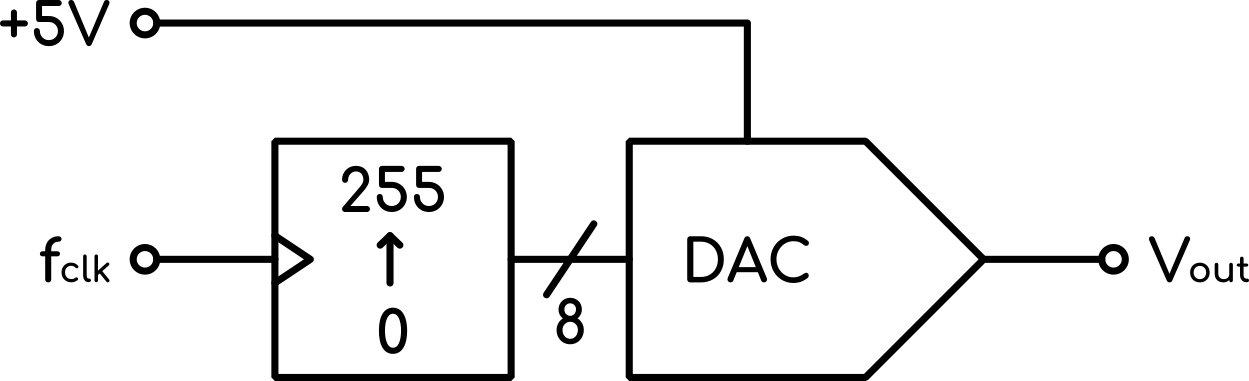
\includegraphics{block_diagrams/ramp_block_diagram.png}
    \caption{Schema a blocchi del sottosistema per la generazione della rampa}
    \label{ramp_block_diagram}
\end{figure}

A questo punto possiamo calcolare le specifiche del segnale di clock da generare,
andando a vedere quali sono le frequenze desiderate per i segnali audio:

\begin{itemize}
    \item Valore minimo (nota A0): $f_{signal-min}=27.5\ Hz\rightarrow f_{clk-min}\approx7\ kHz$
          a cui corrisponderà un ingresso di $0\ V$;
    \item Valore massimo (nota A8): $f_{signal-max}\approx7\ kHz\rightarrow f_{clk-max}\approx1.8\ MHz$
          a cui corrisponderà un ingresso di $+8\ V$;
\end{itemize}

quindi un range di funzionamento esteso lungo 8 ottave.

%--------------------------------------------------------------------------------------------

\subsection*{Componenti Utilizzati e Schemi Elettrici}

%--------------------------------------------------------------------------------------------

Si passa ora alla scelta dei componenti per la realizzazione del blocco circuitale.

\begin{itemize}
    \item Contatore: 74HC590 \cite{74hc590};
    \item DAC: DAC0800 \cite{dac0800};
\end{itemize}

Per il circuito DAC si utilizza lo schema a pg.10 del relativo datasheet del componente.
Tale configurazione ci permette di convertire il dato binario in un valore compreso
nell'intervallo $\pm V_{ref}$, tuttavia si utilizzano un amplificatore operazionale e dei
resistori di valore differente (rispettivamente TL074 \cite{tl074} e $R_L=\bar{R_L}=3.3\ k\Omega$).
Si noti che anche $V_{ref}$ viene scelta diversa rispetto allo schema nel datasheet
(ovvero $+5\ V$), in modo da garantire le specifiche di progetto sul segnale in uscita.

\begin{figure}[H]
    \centering
    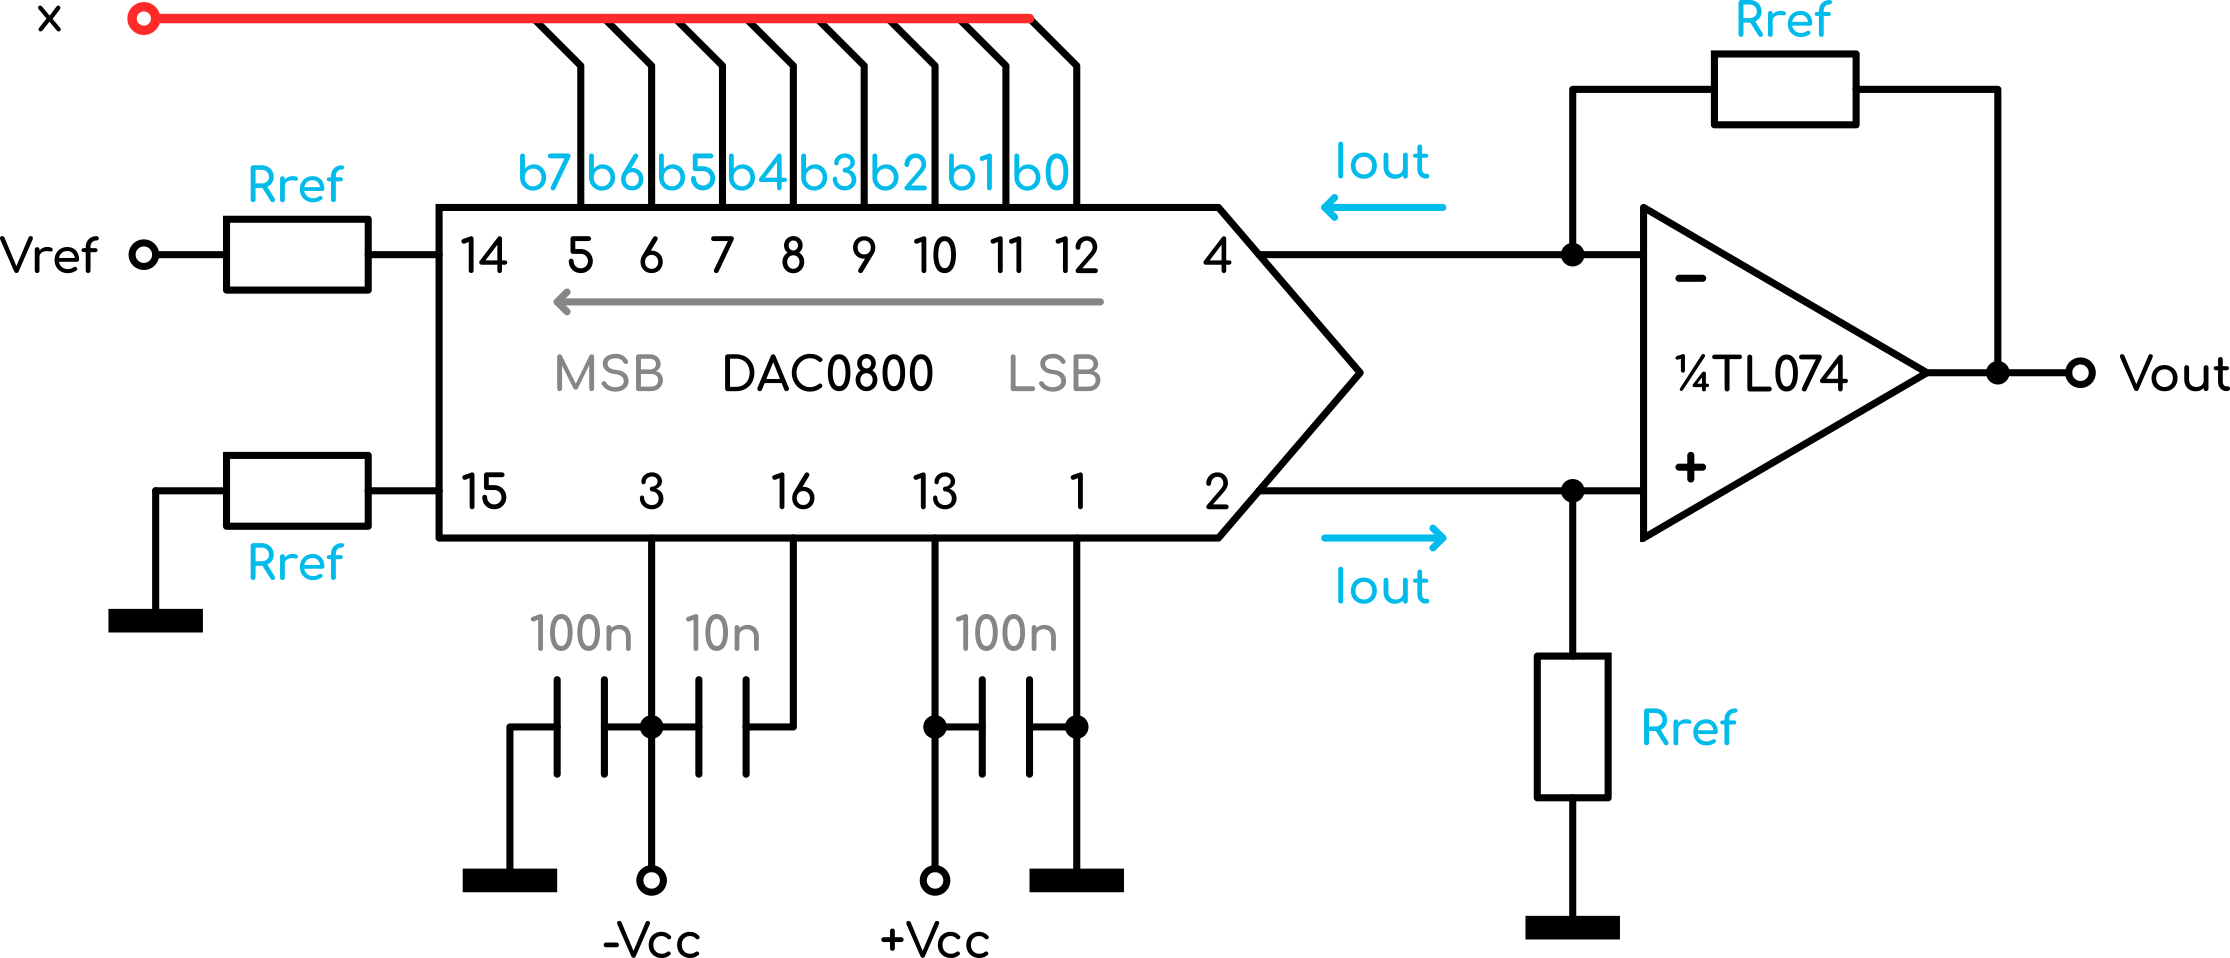
\includegraphics{circuits/DAC_circuit.png}
    \caption{Schema elettrico del DAC ($\pm V_{cc}=\pm 12\ V$)}
    \label{DAC_circuit}
\end{figure}

Il DAC eroga una corrente $I_{out}$ proporzionale all'ingresso digitale $x$, che viene poi
convertita in una tensione con un operazionale. Le due grandezze sono legate dalla relazione:

\begin{equation}\label{vout_dac}
    V_{out}=V_{ref}\left(\frac{2x-255}{256}\right)=5\left(\frac{2x-255}{256}\right)\ [V]
\end{equation}

Il contatore invece viene collegato nel seguente modo:

\begin{figure}[H]
    \centering
    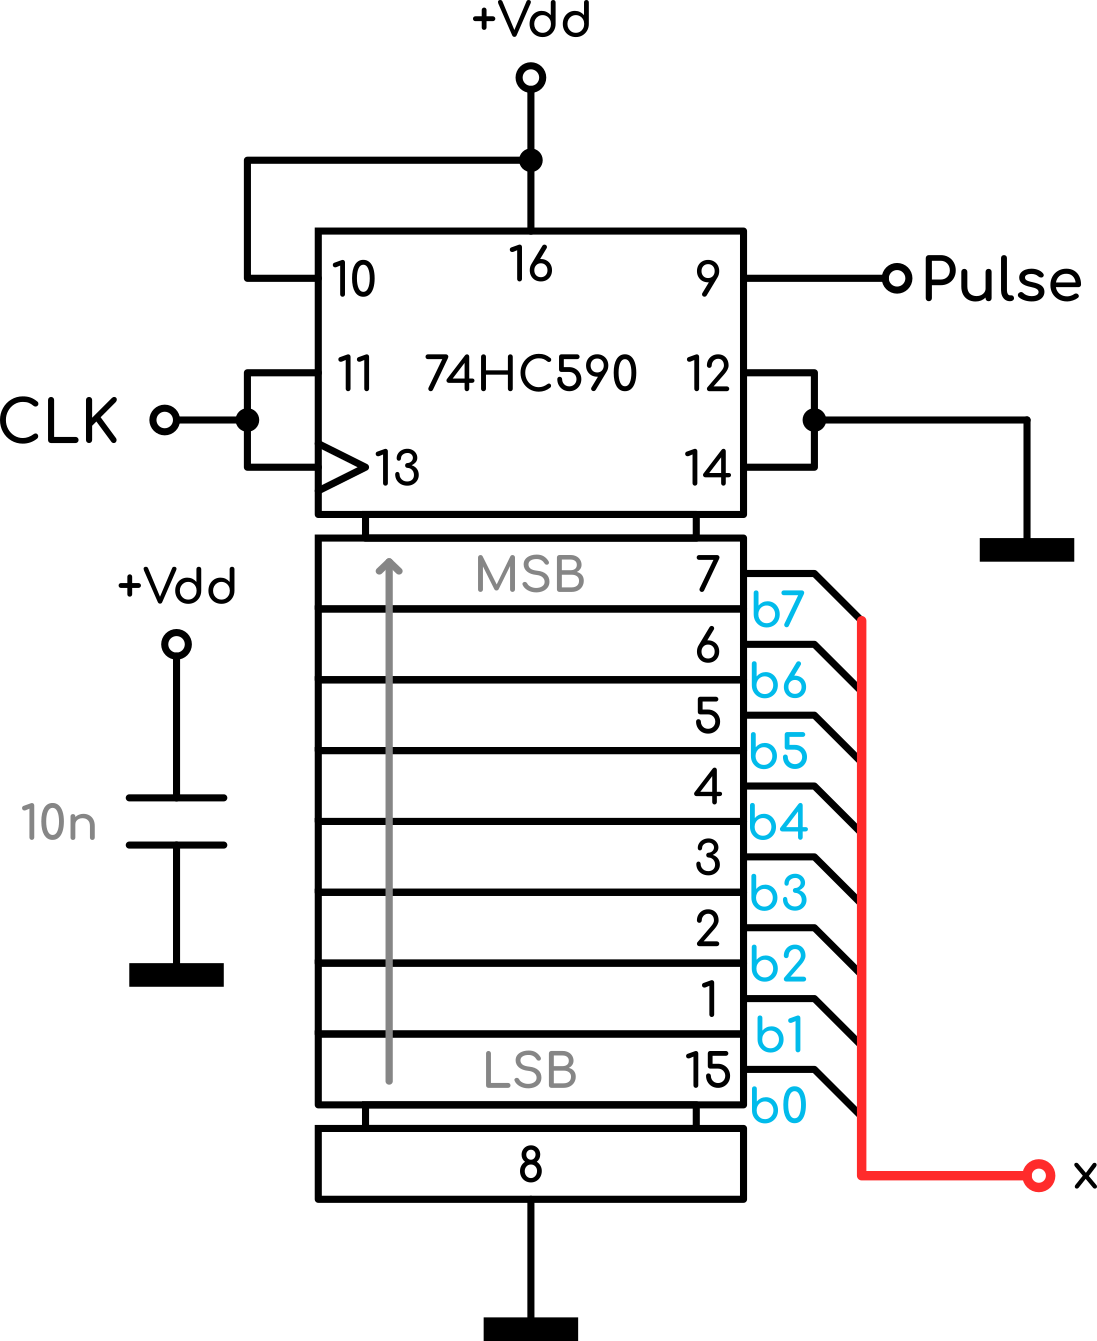
\includegraphics{circuits/ramp_counter_circuit.png}
    \caption{Schema elettrico del contatore per l'onda a rampa, $V_{dd}=+5\ V$}
    \label{ramp_counter_circuit}
\end{figure}

Si noti l'uscita "Pulse" in figura \ref{ramp_counter_circuit} dalla quale viene prelevato
il segnale a impulso precedentemente accennato, discusso più in dettaglio nel capitolo
\ref{segnali_secondari}.

Infine, collegando i due blocchi insieme, l'andamento di $V_{out}$ sarà simile a quello
rappresentato in figura \ref{high_res_ramp}, e ad ogni impulso di clock corrisponderà un
gradino di tensione di circa $40\ mV$ come calcolato con la formula \ref{vstep}.

%--------------------------------------------------------------------------------------------

\subsection*{Risultati Pratici}

%--------------------------------------------------------------------------------------------

Verifichiamo quindi la correttezza del circuito realizzato con il seguente setup di misura:

\begin{figure}[H]
    \centering
    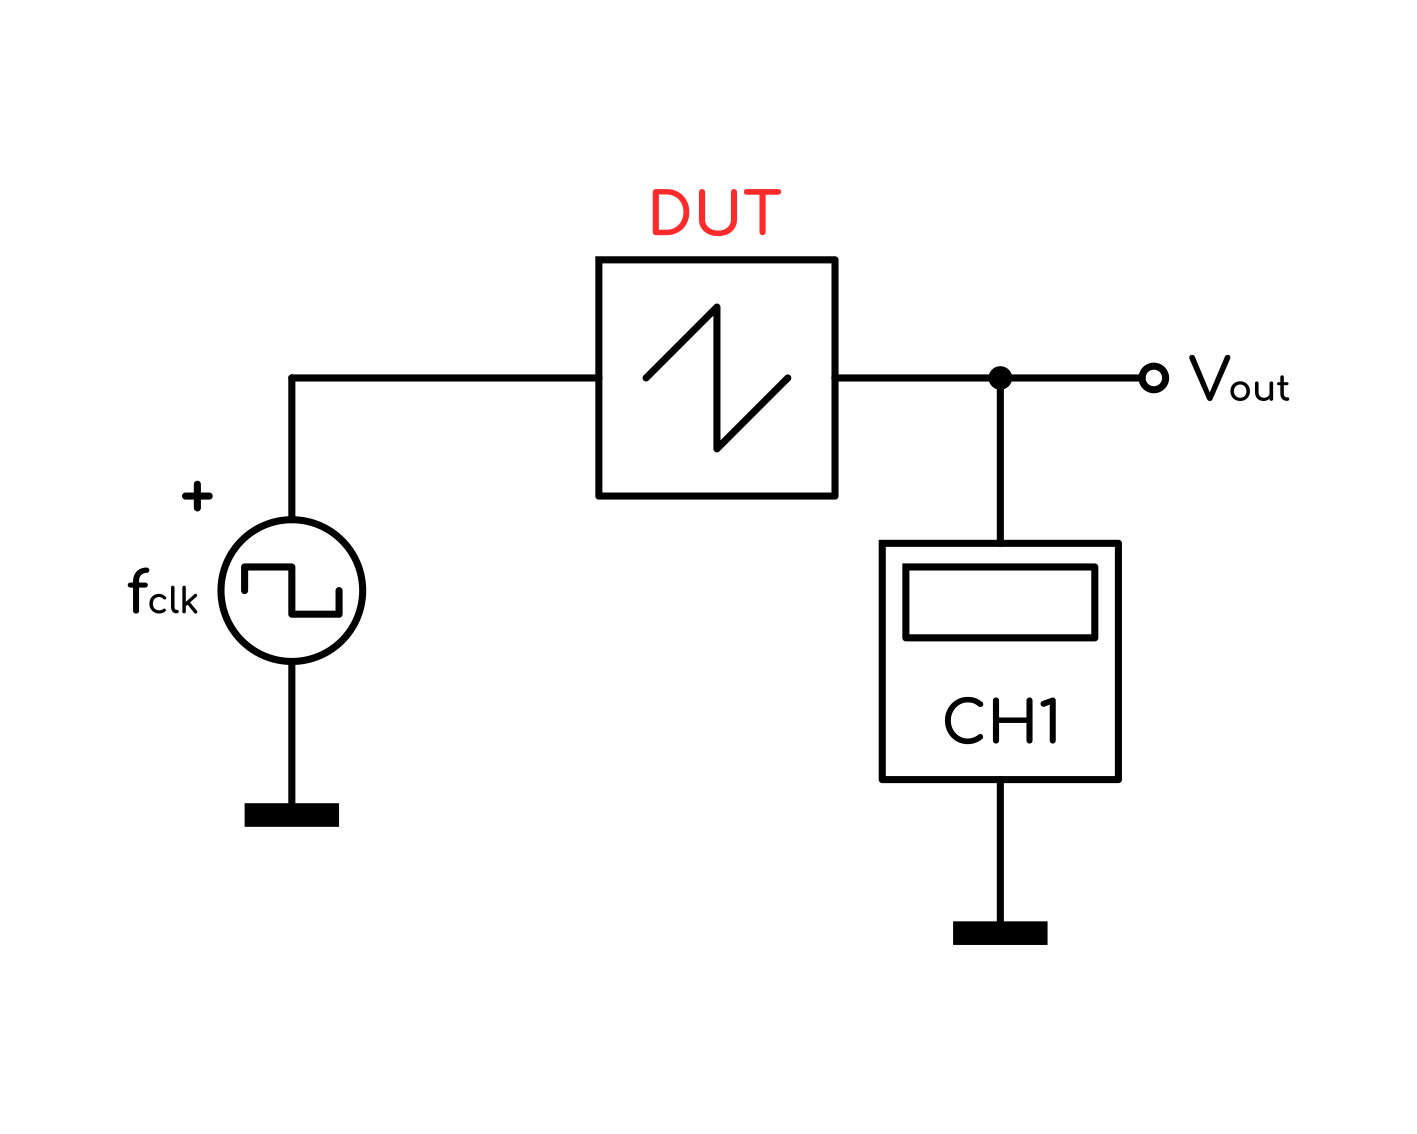
\includegraphics{block_diagrams/mis_ramp.png}
    \caption{Circuito di misura del segnale rampa}
    \label{mis_ramp}
\end{figure}

\vspace{2cm}

Si osservano le seguenti forme d'onda:

\begin{figure}[H]
    \centering

    \begin{subfigure}{.5\textwidth}
        \centering
        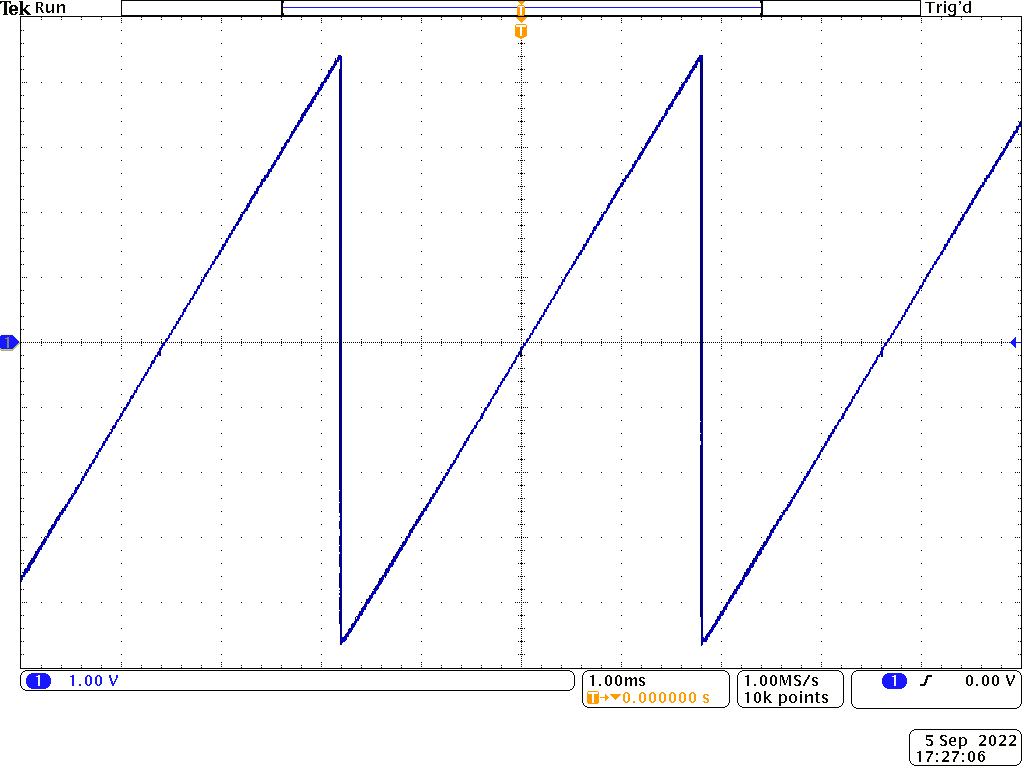
\includegraphics[scale = 0.2]{acquisitions/ramp_wave.png}
        \caption{Acquisizione del segnale a rampa ottenuto}
        \label{acq_ramp}
    \end{subfigure}%
    \begin{subfigure}{.5\textwidth}
        \centering
        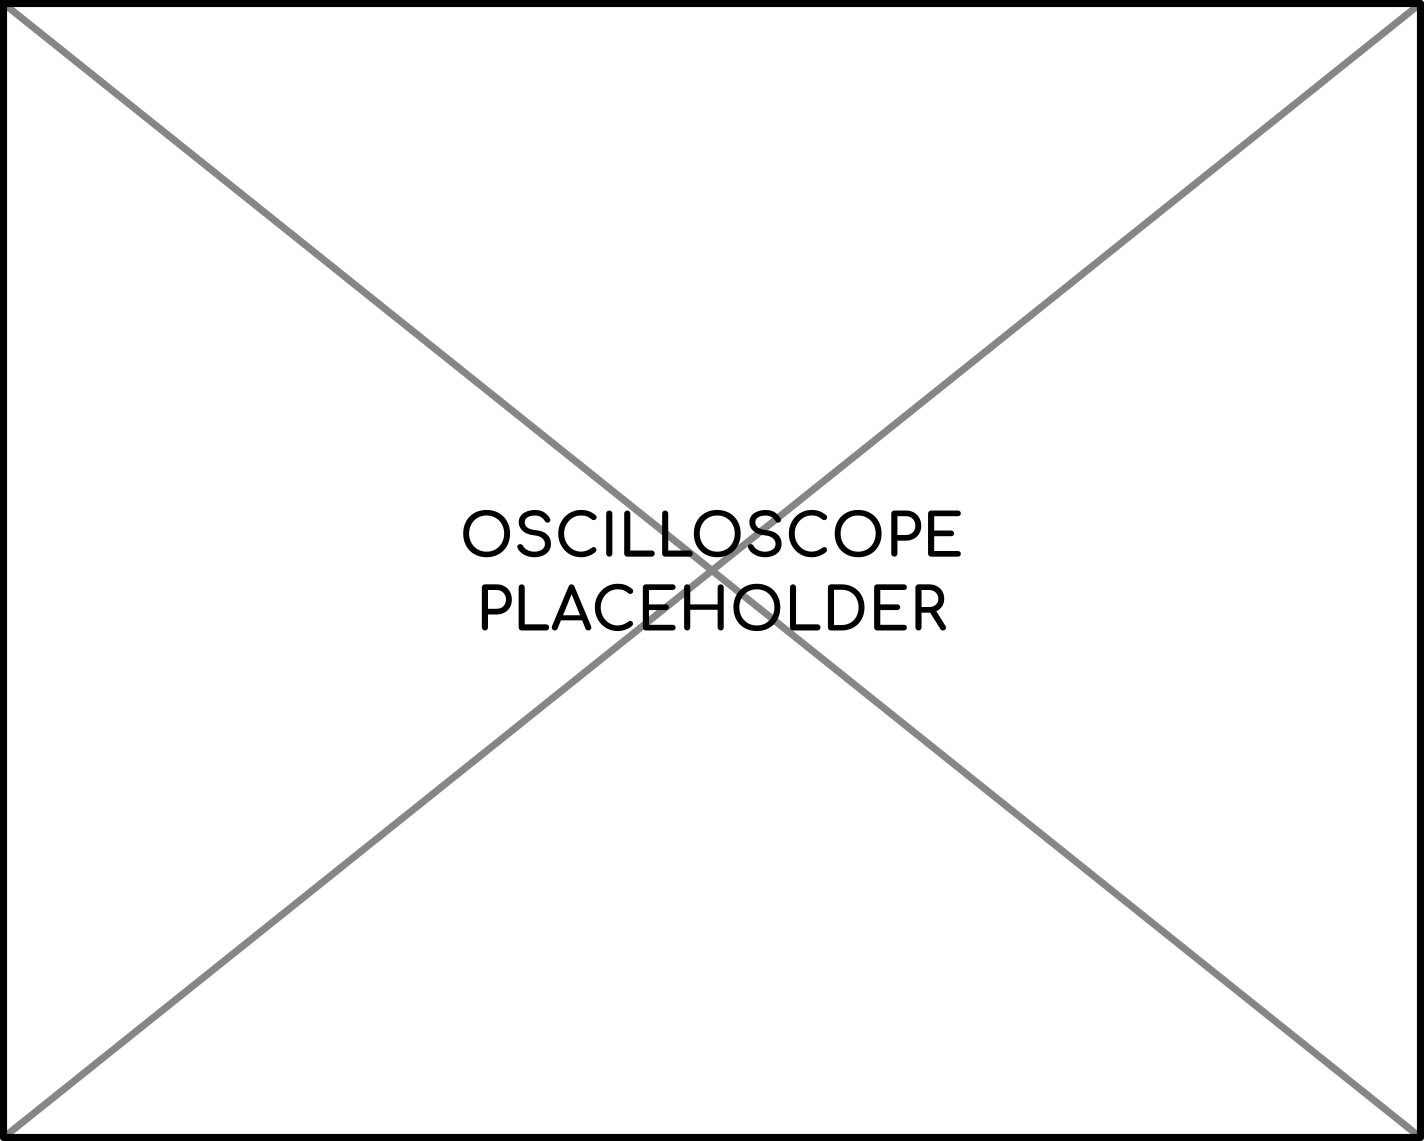
\includegraphics{misc/oscilloscope_placeholder.png}
        \caption{Zoom degli step della rampa e clock}
        \label{acq_ramp_steps}
    \end{subfigure}

    \caption{Correttezza del circuito per il segnale a rampa}
    \label{acq_ramp_signals}
\end{figure}

Si apprezza come l'onda generata abbia esattamente la forma voluta e il comportamento del
contatore in abbinamento al DAC sia come descritto nel principio di funzionamento.

%--------------------------------------------------------------------------------------------

\section{Triangolo}

%--------------------------------------------------------------------------------------------

\subsection*{Principio di Funzionamento}

%--------------------------------------------------------------------------------------------

Il ragionamento è del tutto analogo a quello del contatore per la rampa, tuttavia in questo
caso il contatore utilizzato è bidirezionale (quindi in grado di contare da $0$ a $2^n$ e
viceversa) e necessita di un segnale che determini la direzione di conteggio (Up o Down).

\begin{figure}[H]
    \centering
    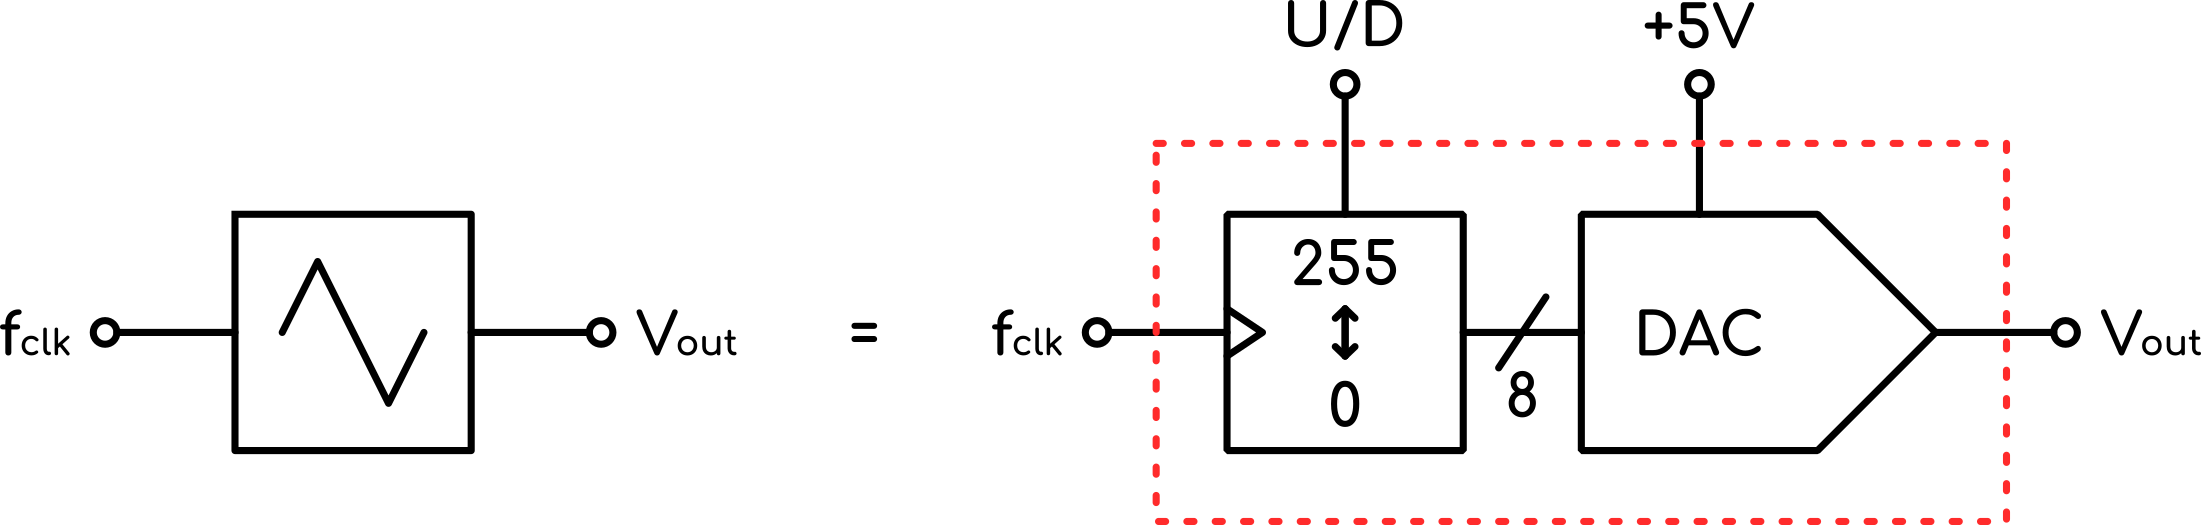
\includegraphics{block_diagrams/triangle_block_diagram.png}
    \caption{Schema a blocchi del sottosistema per la generazione del triangolo}
    \label{triangle_block_diagram}
\end{figure}

\begin{figure}[H]
    \centering

    \begin{subfigure}{.5\textwidth}
        \centering
        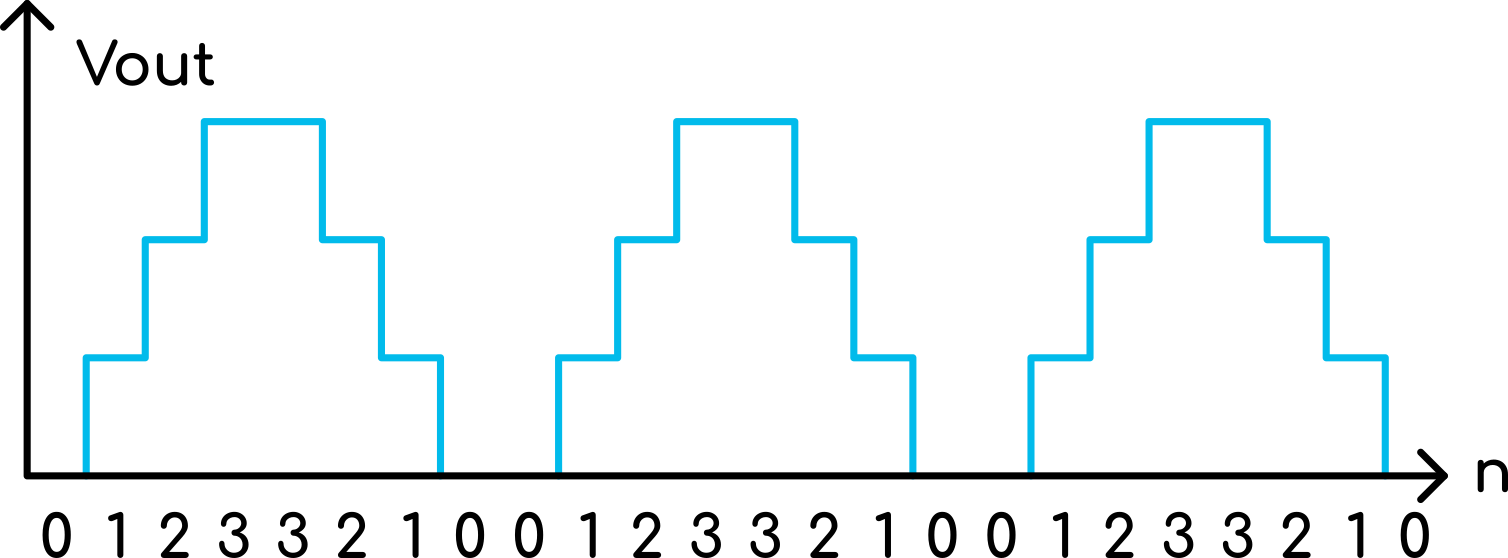
\includegraphics{graphs/low_res_triangle.png}
        \caption{Triangolo ottenuto con un contatore a 2 bit}
        \label{low_res_triangle}
    \end{subfigure}%
    \begin{subfigure}{.5\textwidth}
        \centering
        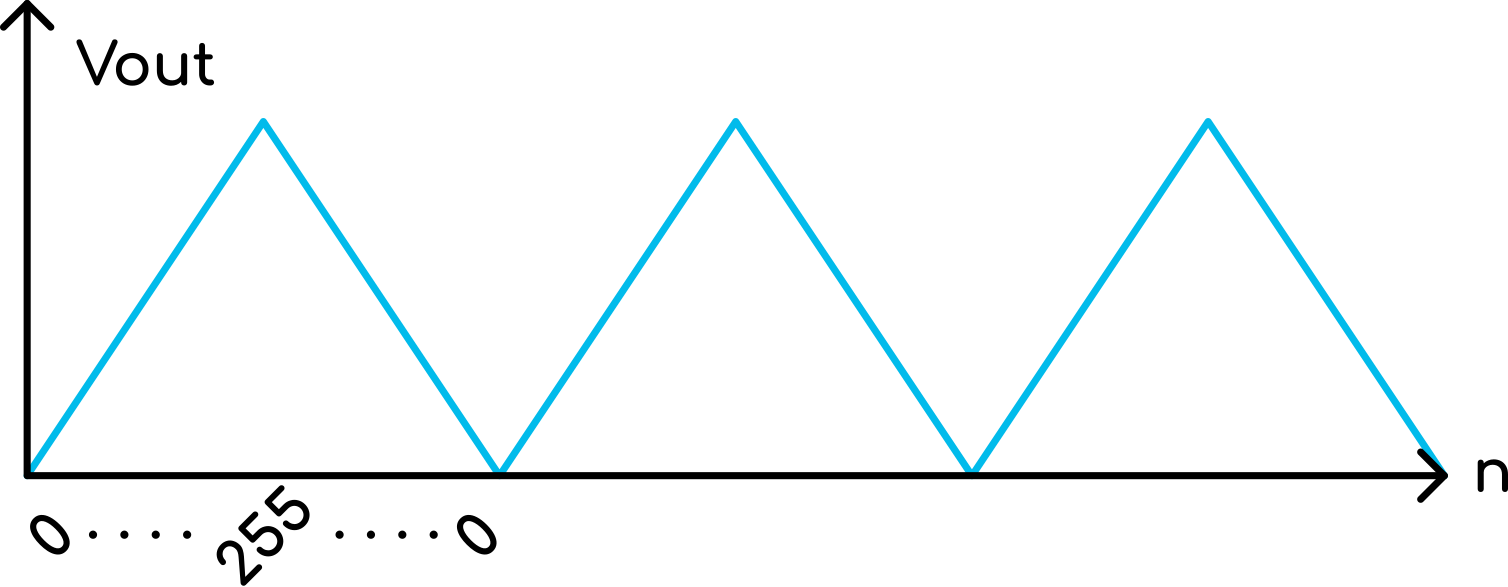
\includegraphics{graphs/high_res_triangle.png}
        \caption{Triangolo ottenuto con un contatore a 8 bit}
        \label{high_res_triangle}
    \end{subfigure}

    \caption{Confronto tra contatori bidirezionali con diverso numero di bit}
    \label{triangles}
\end{figure}

La configurazione del DAC rimane quella utilizzata per la rampa e rappresentata in figura
\ref{DAC_circuit}. In questo caso tuttavia il numero di cicli di clock utilizzati è doppio
rispetto a quello per la rampa, poichè dovranno essere eseguiti 256 conteggi verso l'alto
e 256 conteggi verso il basso per ottenere un singolo periodo di onda triangolare. Ne
consegue quindi che anche la frequenza di clock in ingresso a questo sottosistema dovrà
essere doppia rispetto alla rampa, come risulta evidente in figura \ref{steps}.

\begin{figure}[H]
    \centering

    \begin{subfigure}{.5\textwidth}
        \centering
        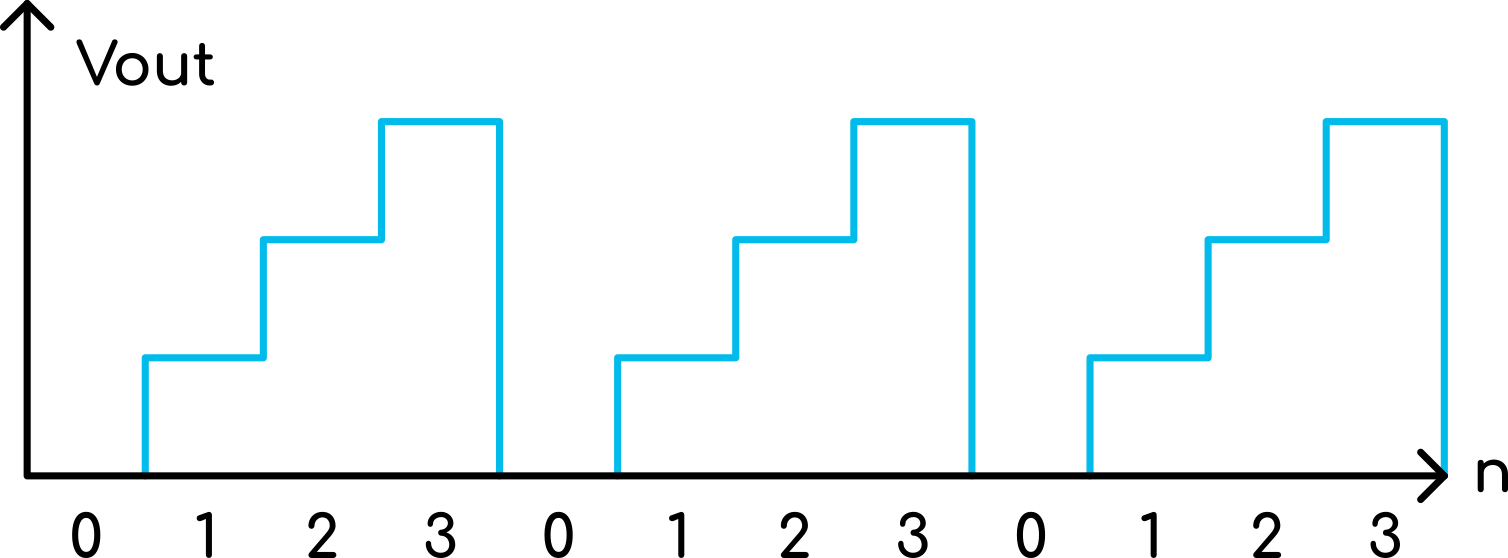
\includegraphics{graphs/low_res_ramp.png}
        \caption{Rampa ottenuta con un contatore a 2 bit}
    \end{subfigure}%
    \begin{subfigure}{.5\textwidth}
        \centering
        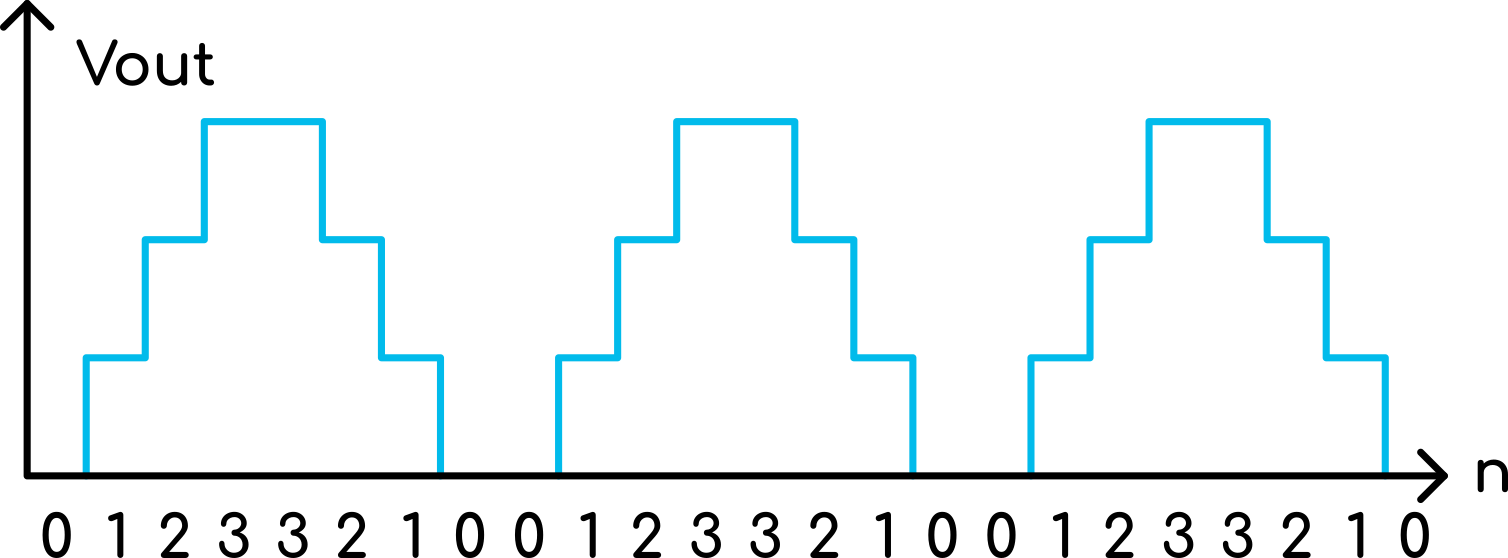
\includegraphics{graphs/low_res_triangle.png}
        \caption{Triangolo ottenuto con un contatore a 2 bit}
    \end{subfigure}

    \caption{Confronto del conteggio tra contatori unidirezionali (a) e bidirezionali (b)}
    \label{steps}
\end{figure}

%--------------------------------------------------------------------------------------------

\subsection*{Componenti Utilizzati e Schemi Elettrici}

%--------------------------------------------------------------------------------------------

L'unico componente diverso rispetto al circuito per la rampa è il contatore, che come già
detto deve essere bidirezionale. Si utilizzano due 74LS169 \cite{74ls169} in cascata nella
seguente configurazione:

\begin{figure}[H]
    \centering
    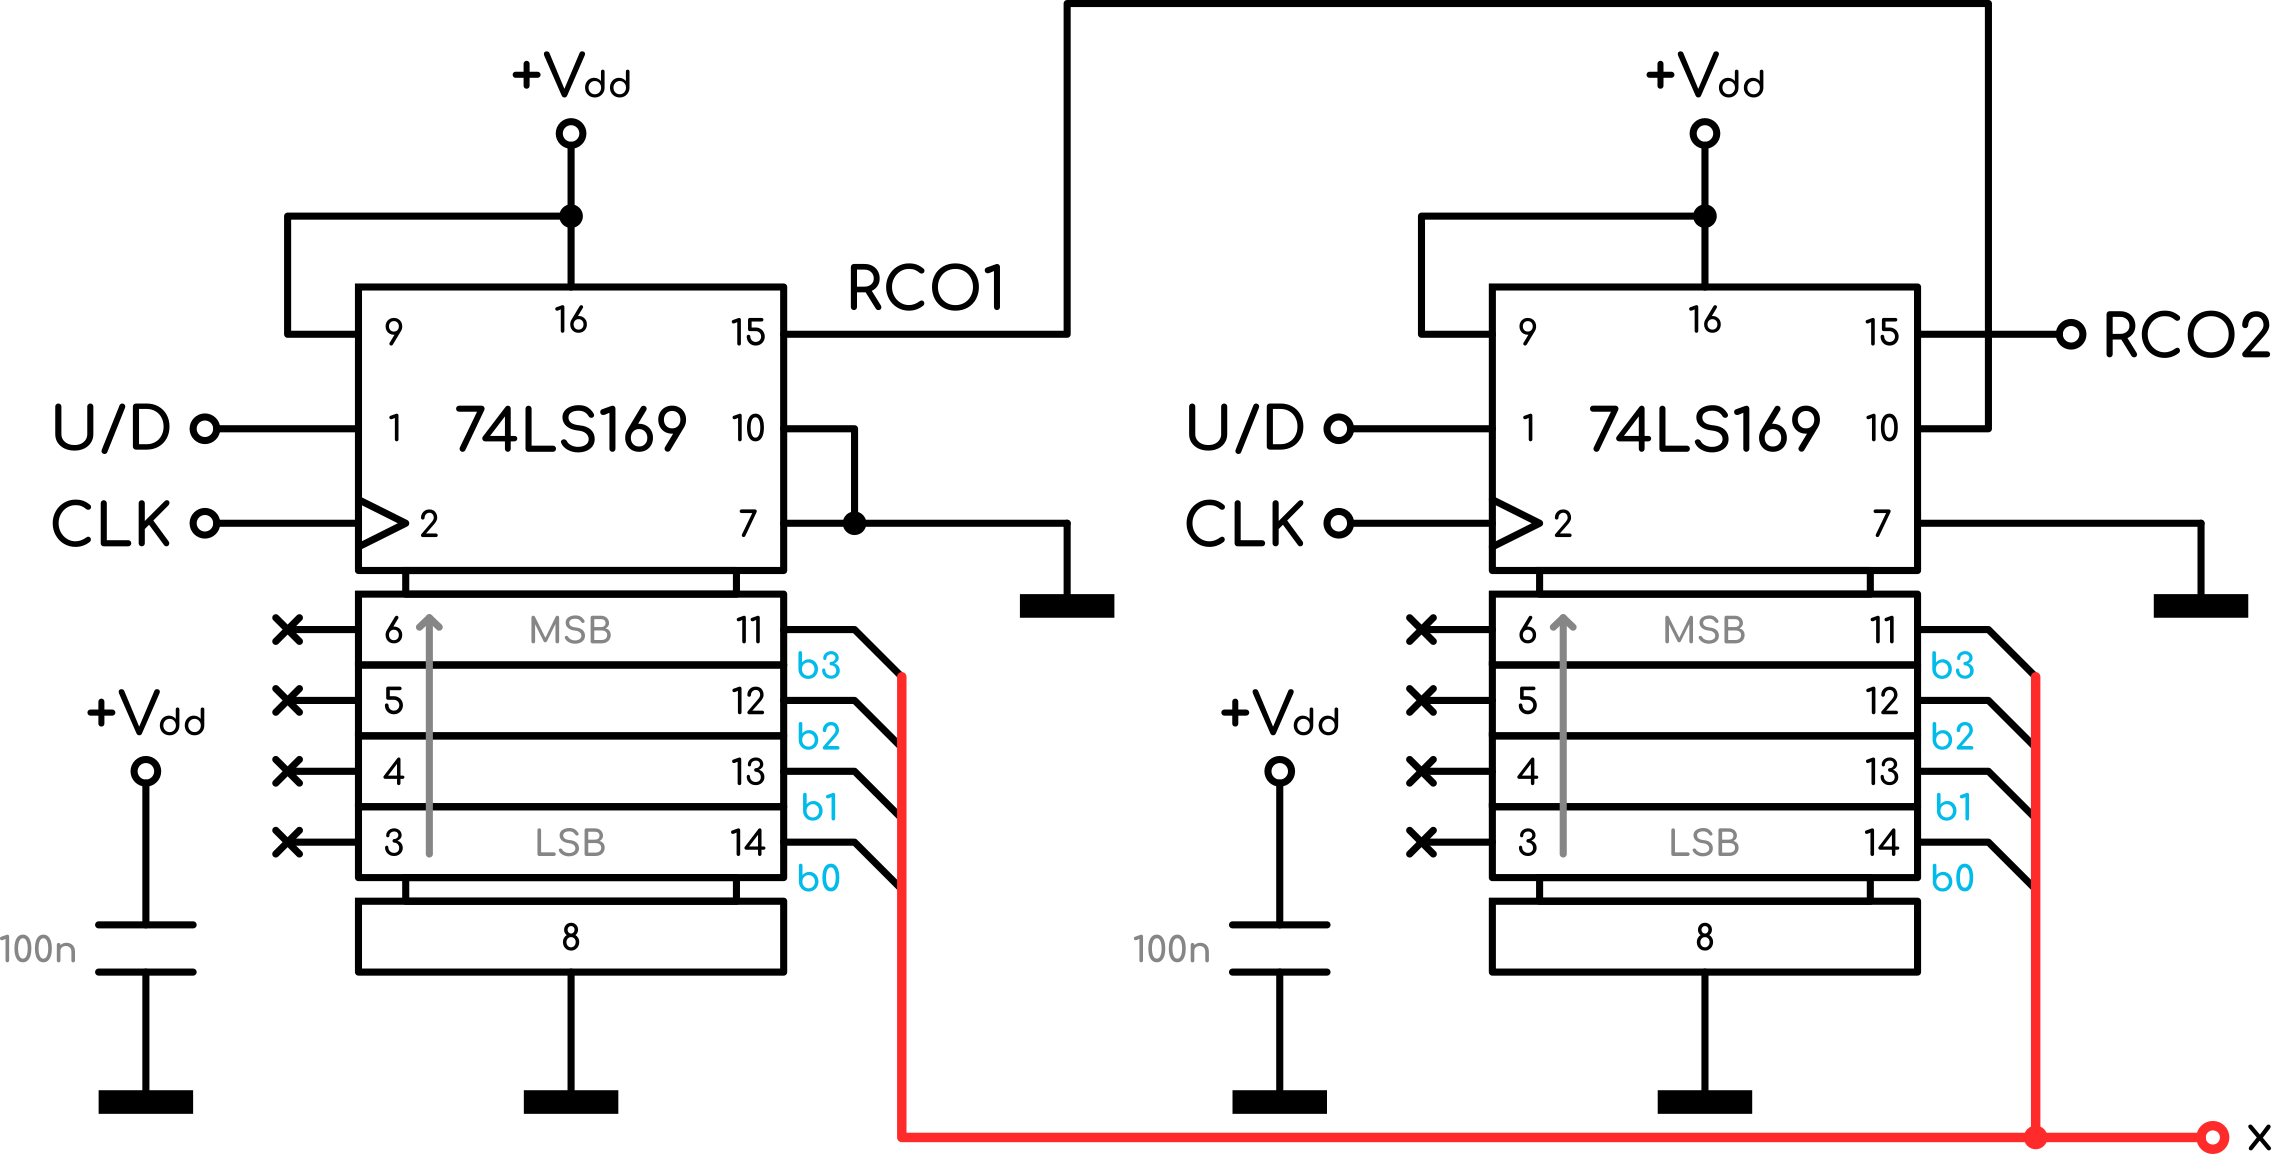
\includegraphics{circuits/triangle_counter_circuit.png}
    \caption{Schema elettrico dei contatori per l'onda triangolare ($V_{dd}=+5\ V$)}
    \label{triangle_counter_circuit}
\end{figure}

Il componente utilizzato presenta anche degli ingressi per il preset del numero di partenza
(pin da 3 a 6), che però nel nostro caso non vengono utilizzati.

L'uscita denominata $RCO2$ verrà utilizzata per pilotare il verso del conteggio, essa infatti
commuta durante il ciclo di clock corrispondente al conteggio precedente all'overflow, ovvero
$255$ in modalità "Up" e $0$ in modalità "Down".

\begin{figure}[H]
    \centering
    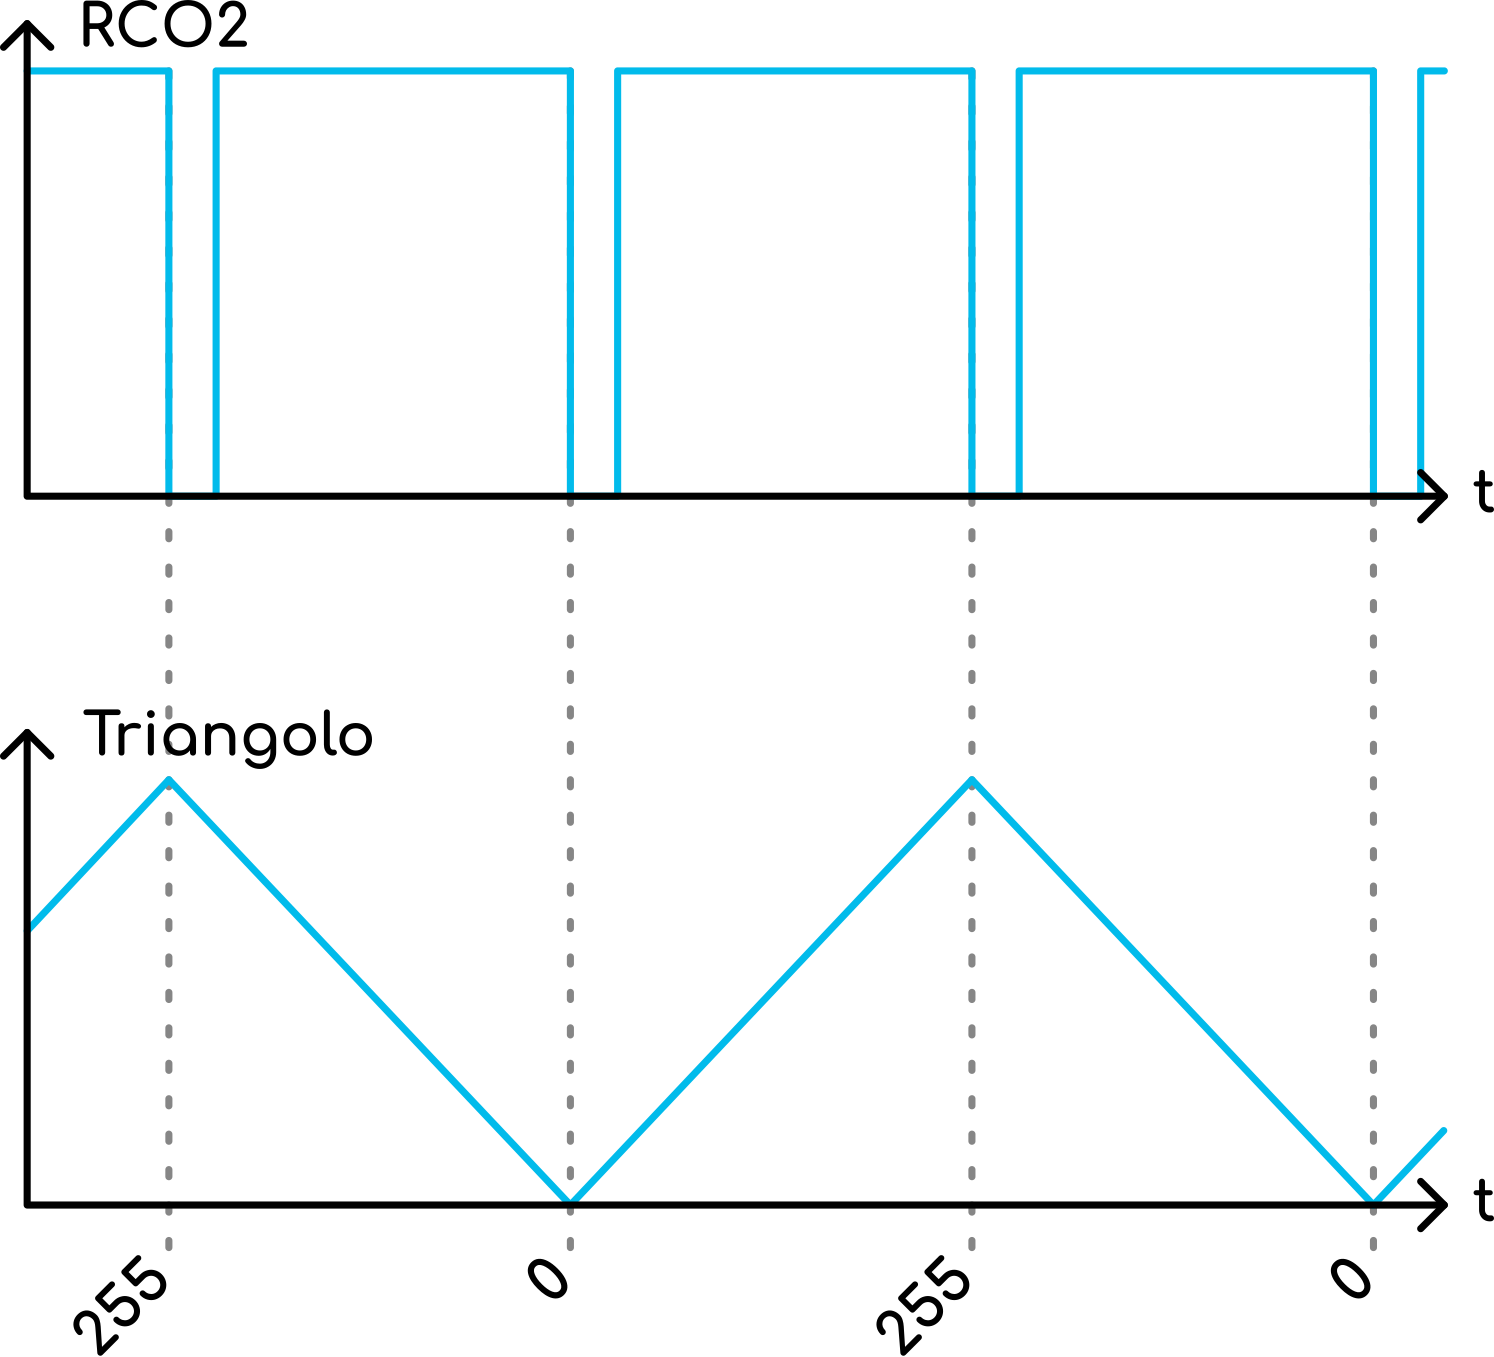
\includegraphics{graphs/RCO2_behaviour.png}
    \caption{Andamento teorico del segnale $RCO2$ in funzione del conteggio}
    \label{RCO2_behaviour}
\end{figure}

%--------------------------------------------------------------------------------------------

\subsection*{Risultati Pratici}

%--------------------------------------------------------------------------------------------

Si verifica ora la correttezza del circuito realizzato utilizzando il setup di misura seguente:

\begin{figure}[H]
    \centering
    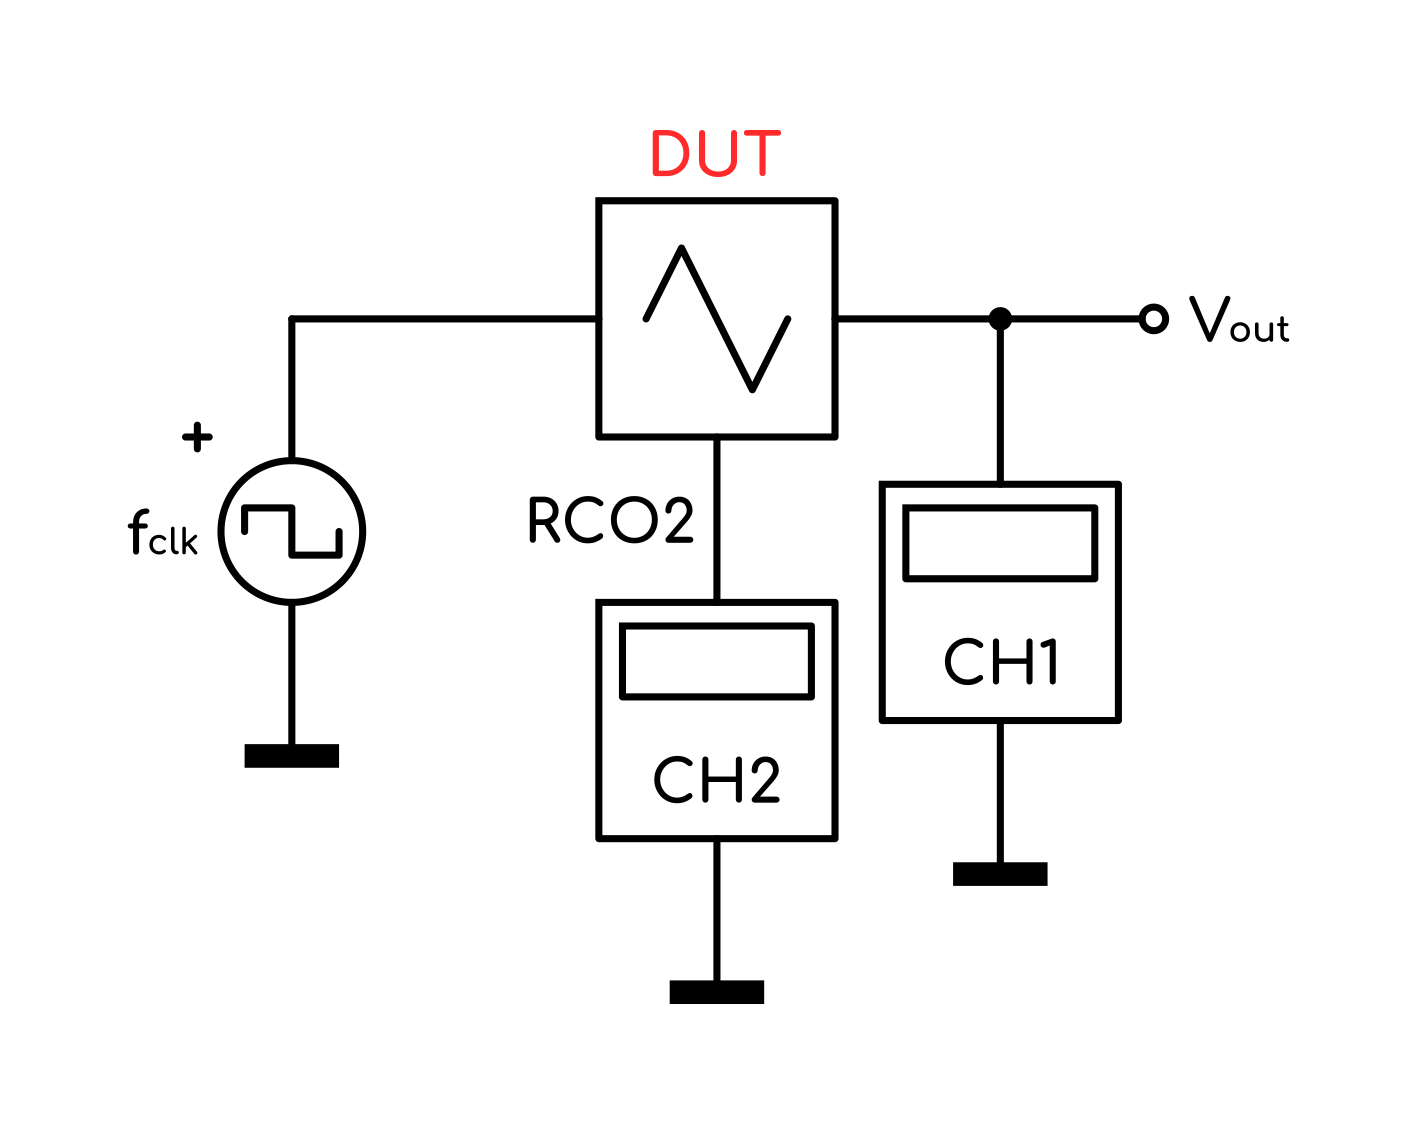
\includegraphics{block_diagrams/mis_triangle.png}
    \caption{Circuito di misura del segnale triangolo}
    \label{mis_triangle}
\end{figure}

e si osservano le seguenti forme d'onda:

\begin{figure}[H]
    \centering

    \begin{subfigure}{.5\textwidth}
        \centering
        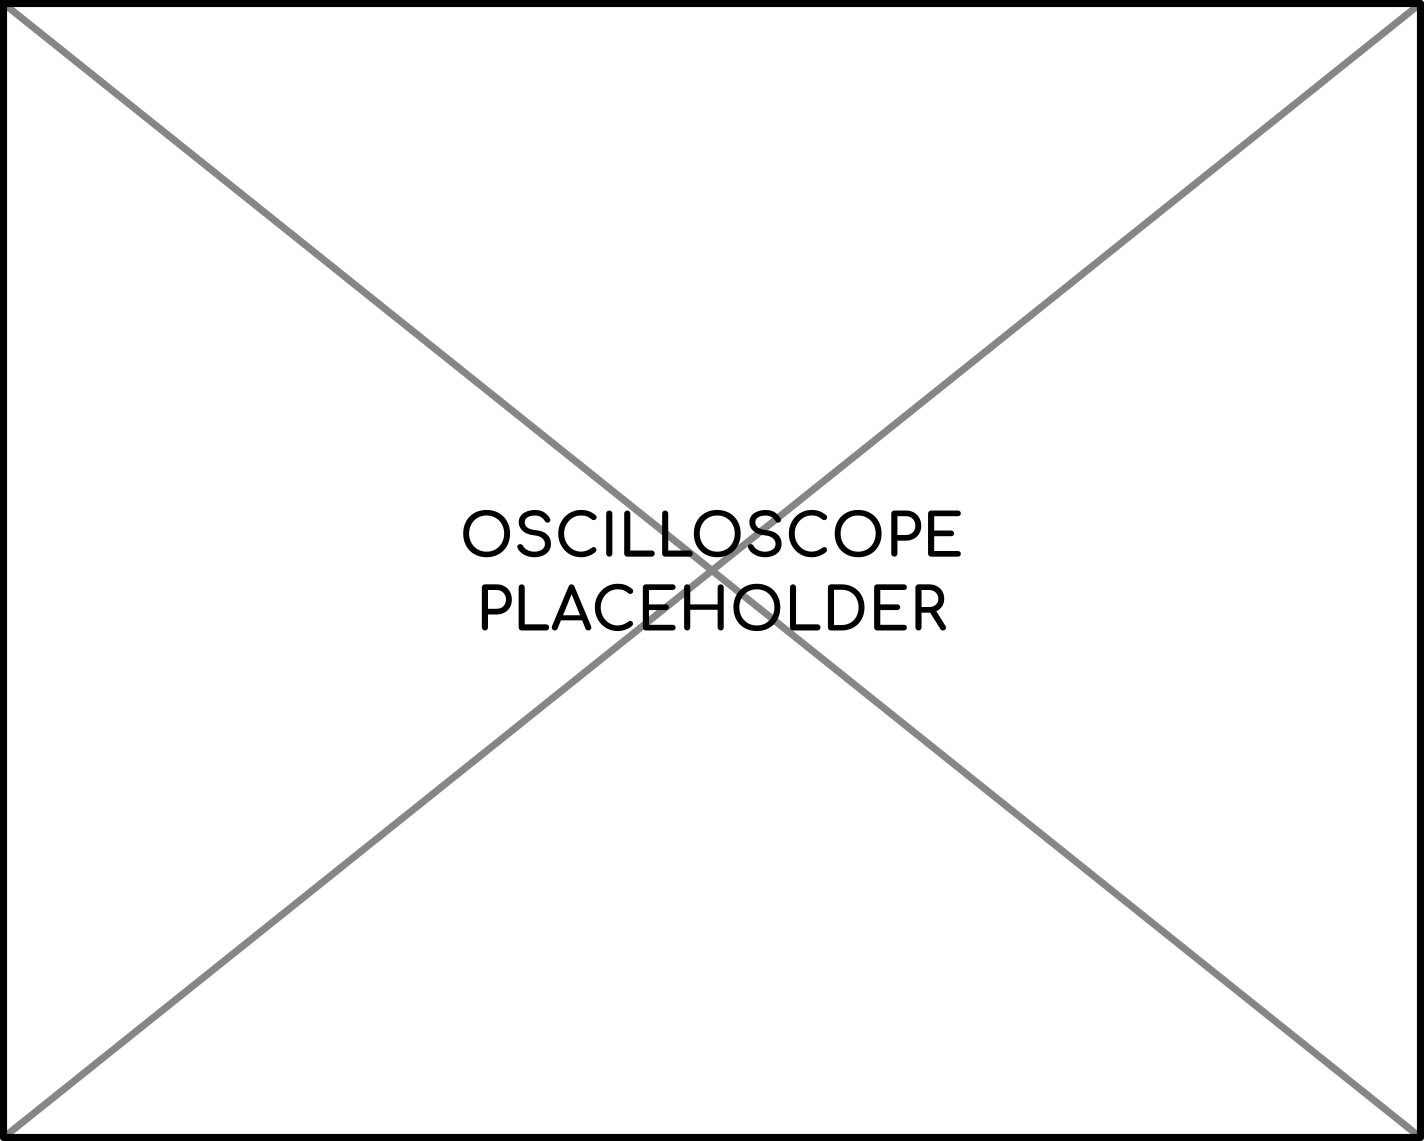
\includegraphics{misc/oscilloscope_placeholder.png}
        \caption{Acquisizione del segnale a triangolo ottenuto}
        \label{acq_triangle}
    \end{subfigure}%
    \begin{subfigure}{.5\textwidth}
        \centering
        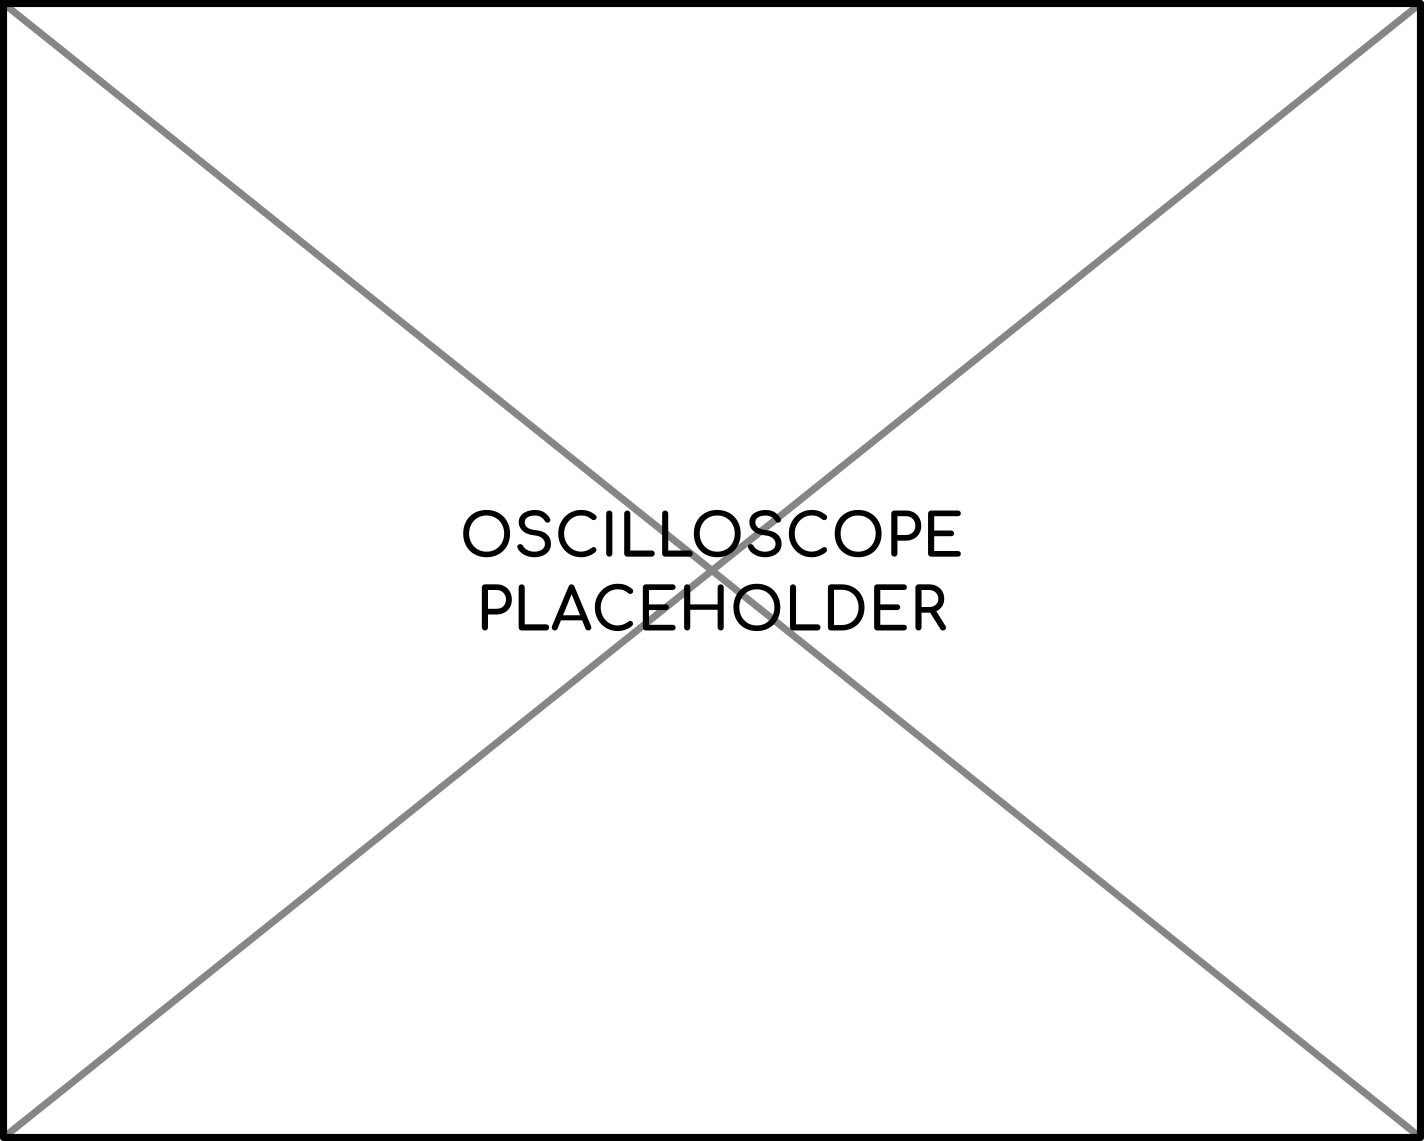
\includegraphics{misc/oscilloscope_placeholder.png}
        \caption{Zoom degli step del triangolo e clock}
        \label{acq_triangle_steps}
    \end{subfigure}

    \caption{Correttezza del circuito per il segnale a triangolo}
    \label{acq_triangle_signals}
\end{figure}

Ancora una volta si apprezza che quanto discusso finora corrisponde al reale comportamento
del circuito.

%--------------------------------------------------------------------------------------------

\section{Adattamento dei Segnali di Clock e Pilotaggio}

%--------------------------------------------------------------------------------------------

Si è visto come, per avere la stessa frequenza di segnale d'uscita, il contatore del
triangolo deve avere una frequenza di clock doppia rispetto a quella del contatore della
rampa. Questo problema si risolve facilmente inserendo prima del contatore unidirezionale
un divisore di frequenza, ottenuto con un semplice toggle flip-flop (TFF).

\begin{figure}[H]
    \centering
    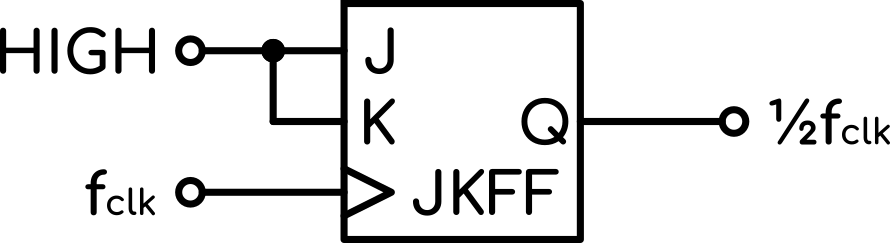
\includegraphics{block_diagrams/freq_divider_block_diagram.png}
    \caption{Schema a blocchi del divisore di frequenza}
    \label{freq_divider_block_diagram}
\end{figure}

\begin{figure}[H]
    \centering
    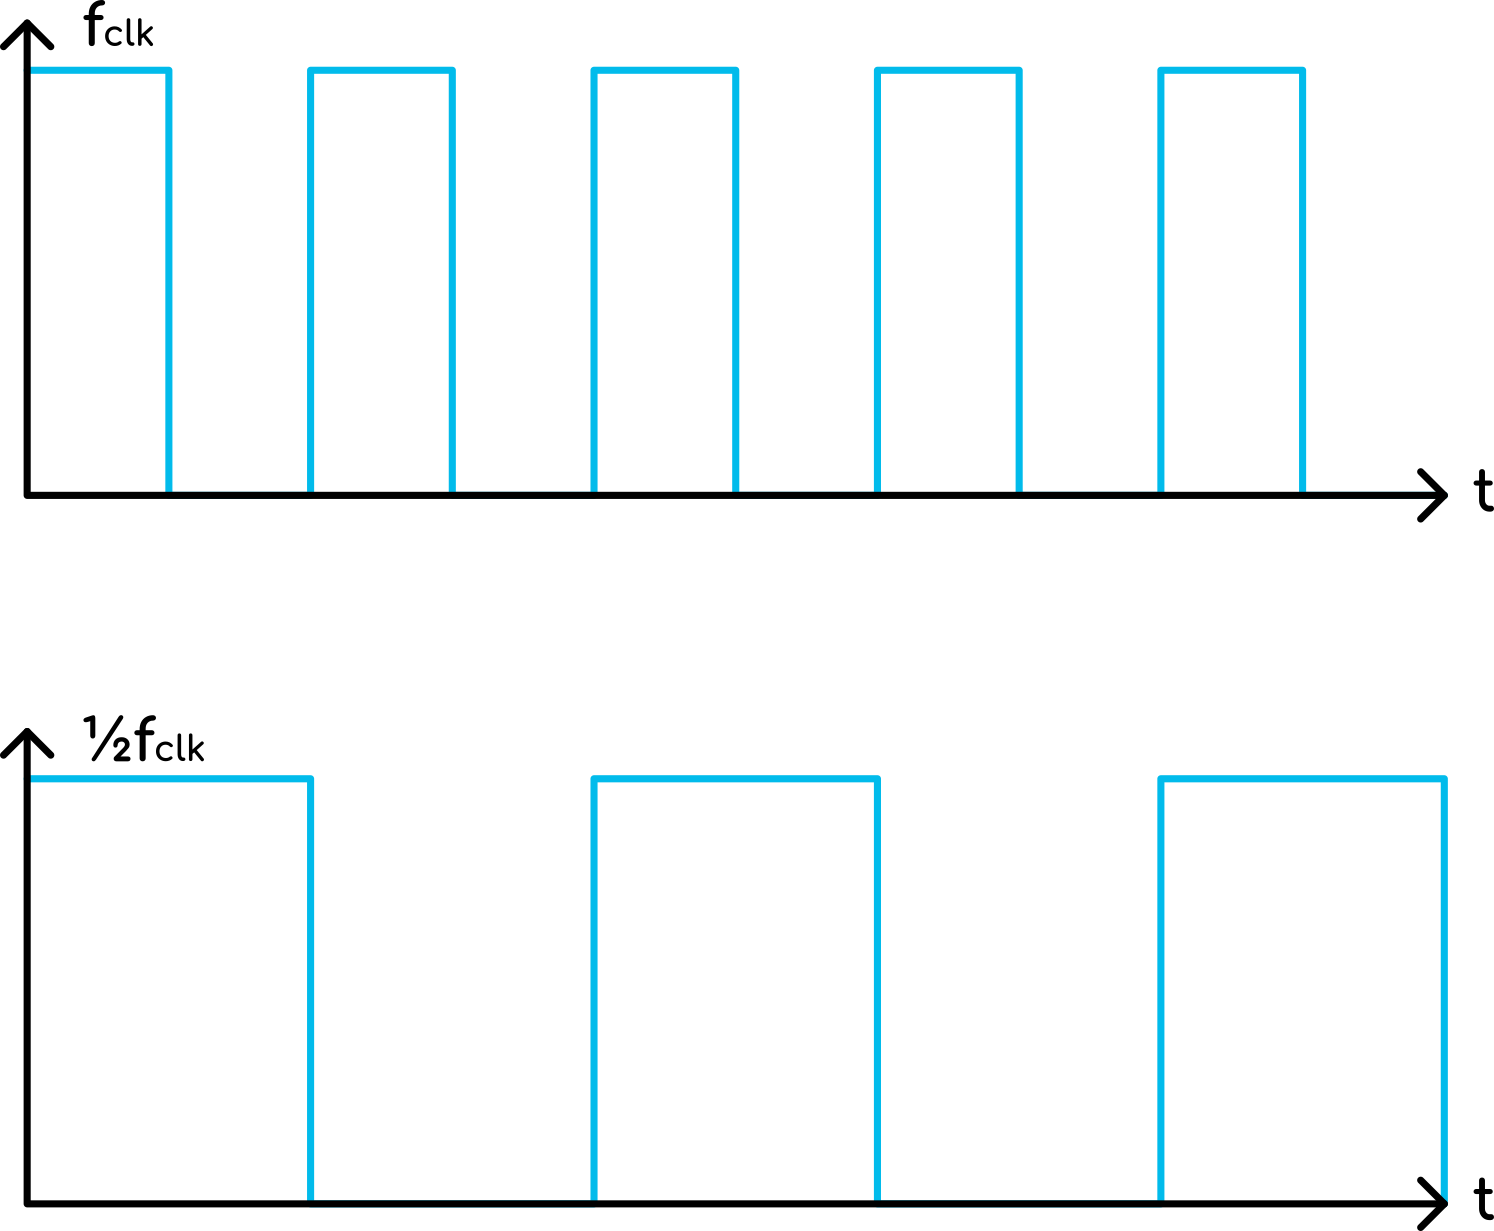
\includegraphics{graphs/clock_divider_behaviour.png}
    \caption{$f_{clk}$ e ½$f_{clk}$ nel divisore di frequenza}
    \label{clock_divider_behaviour}
\end{figure}

Le specifiche sul segnale di clock ci impongono allora di generare un segnale a onda rettangolare
con frequenza variabile nel range $(14\ kHz\div3.6\ MHz)$, in modo che ½$f_{clk}$ abbia
i valori di frequenza inizialmente calcolati.

Invece, per fare in modo che il contatore del triangolo cambi effettivamente verso di conteggio
è necessario impiegare un altro TFF utilizzando come ingresso $\overline{RCO2}$ (poichè
attivo a livello logico basso) e connesso all'ingresso $U/D$ del contatore.

\begin{figure}[H]
    \centering
    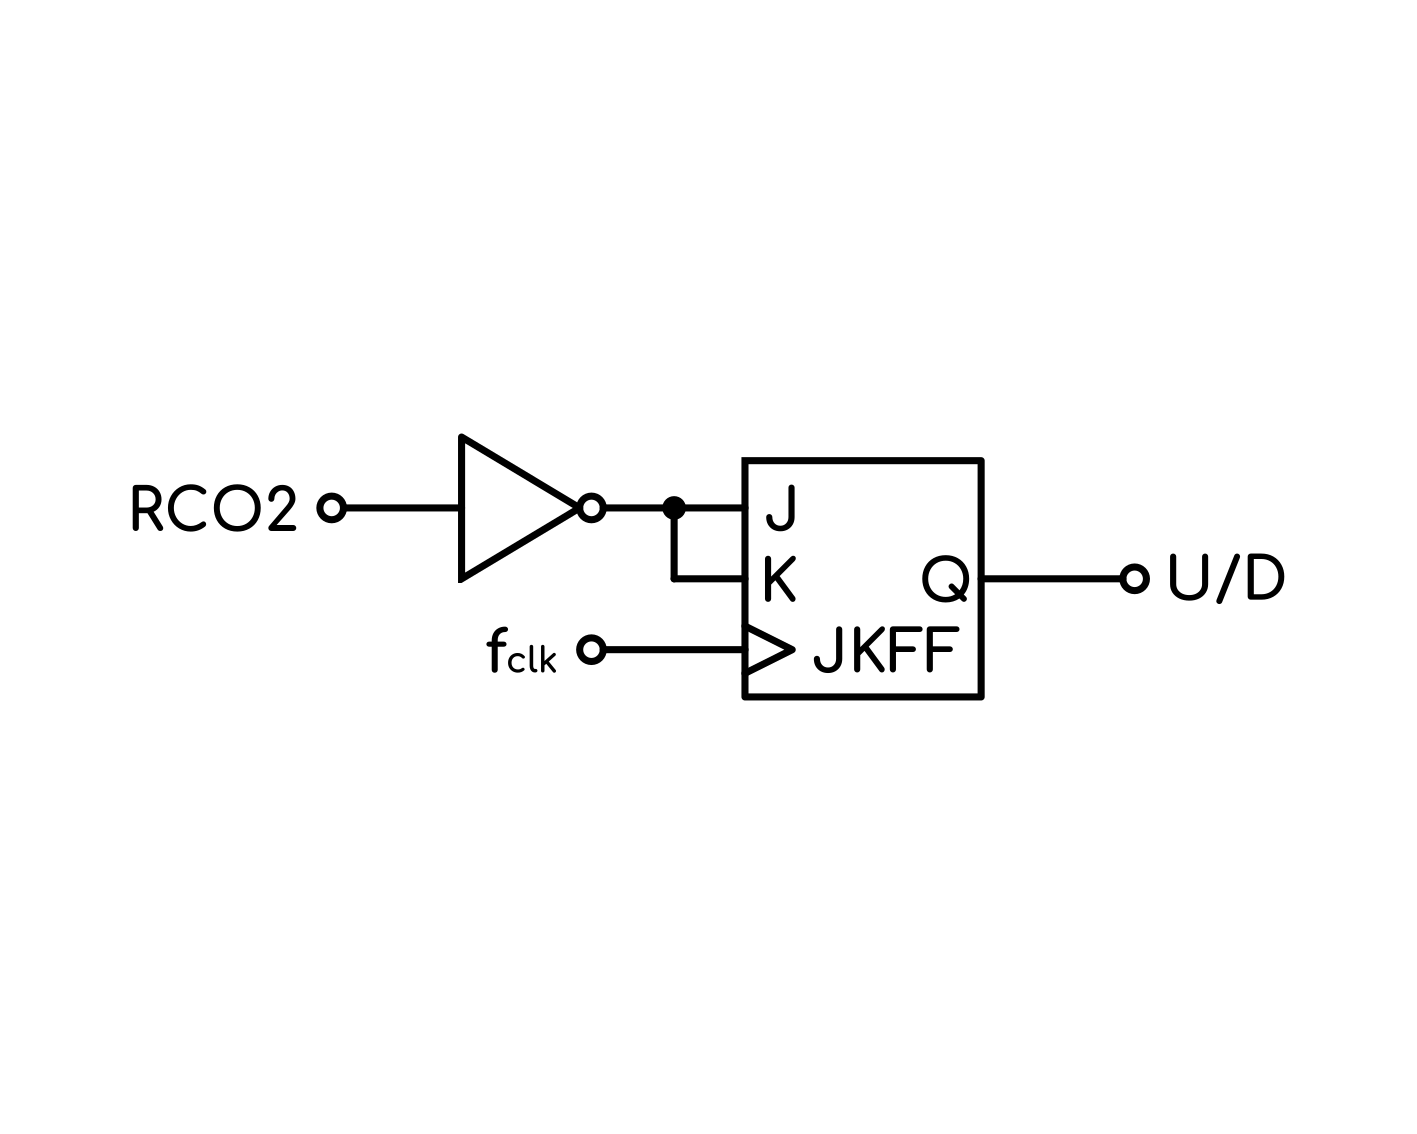
\includegraphics{block_diagrams/UD_block_diagram.png}
    \caption{Schema a blocchi del sistema per il segnale di pilotaggio}
    \label{UD_block_diagram}
\end{figure}

I componenti utilizzati per questo scopo sono:

\begin{itemize}
    \item Flip-Flop: 74HC73 \cite{74hc73};
    \item MOSFET: 2N7000 \cite{2n7000};
\end{itemize}

Lo schema elettrico per l'inverter è rappresentato in figura \ref{inverter_circuit}, dove
il MOSFET utilizzato è compatibile con le tensioni logiche presenti nel circuito.

\begin{figure}[H]
    \centering
    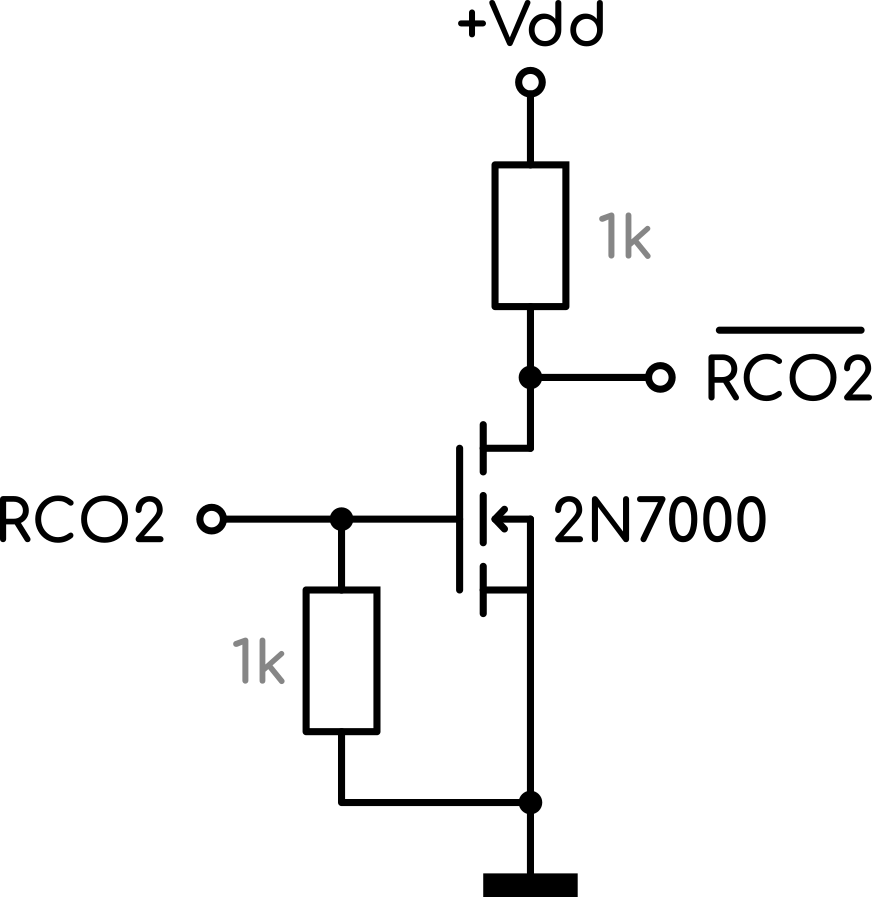
\includegraphics{circuits/inverter_circuit.png}
    \caption{Schema elettrico dell'inverter logico ($V_{dd}=+5\ V$)}
    \label{inverter_circuit}
\end{figure}

%--------------------------------------------------------------------------------------------

\subsection*{Risultati Pratici}

%--------------------------------------------------------------------------------------------

Si verifica la correttezza dei circuiti:

\begin{figure}[H]
    \centering

    \begin{subfigure}{.5\textwidth}
        \centering
        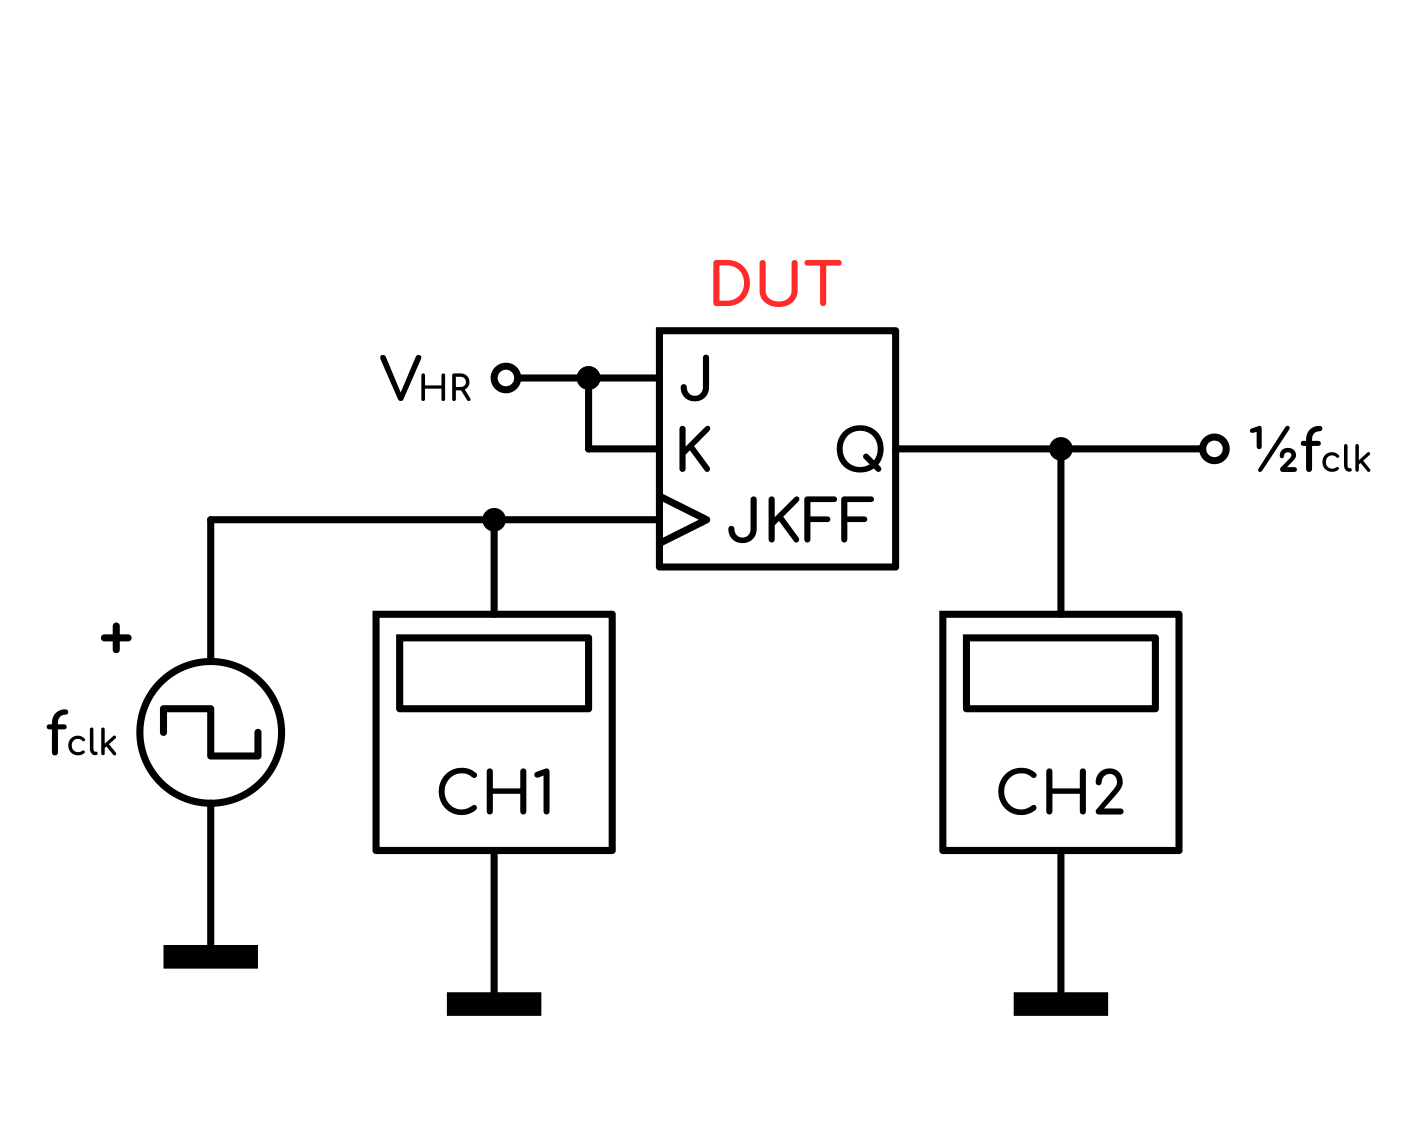
\includegraphics{block_diagrams/mis_clock_divider.png}
        \caption{Circuito di misura del divisore di frequenza}
        \label{mis_clock_divider}
    \end{subfigure}%
    \begin{subfigure}{.5\textwidth}
        \centering
        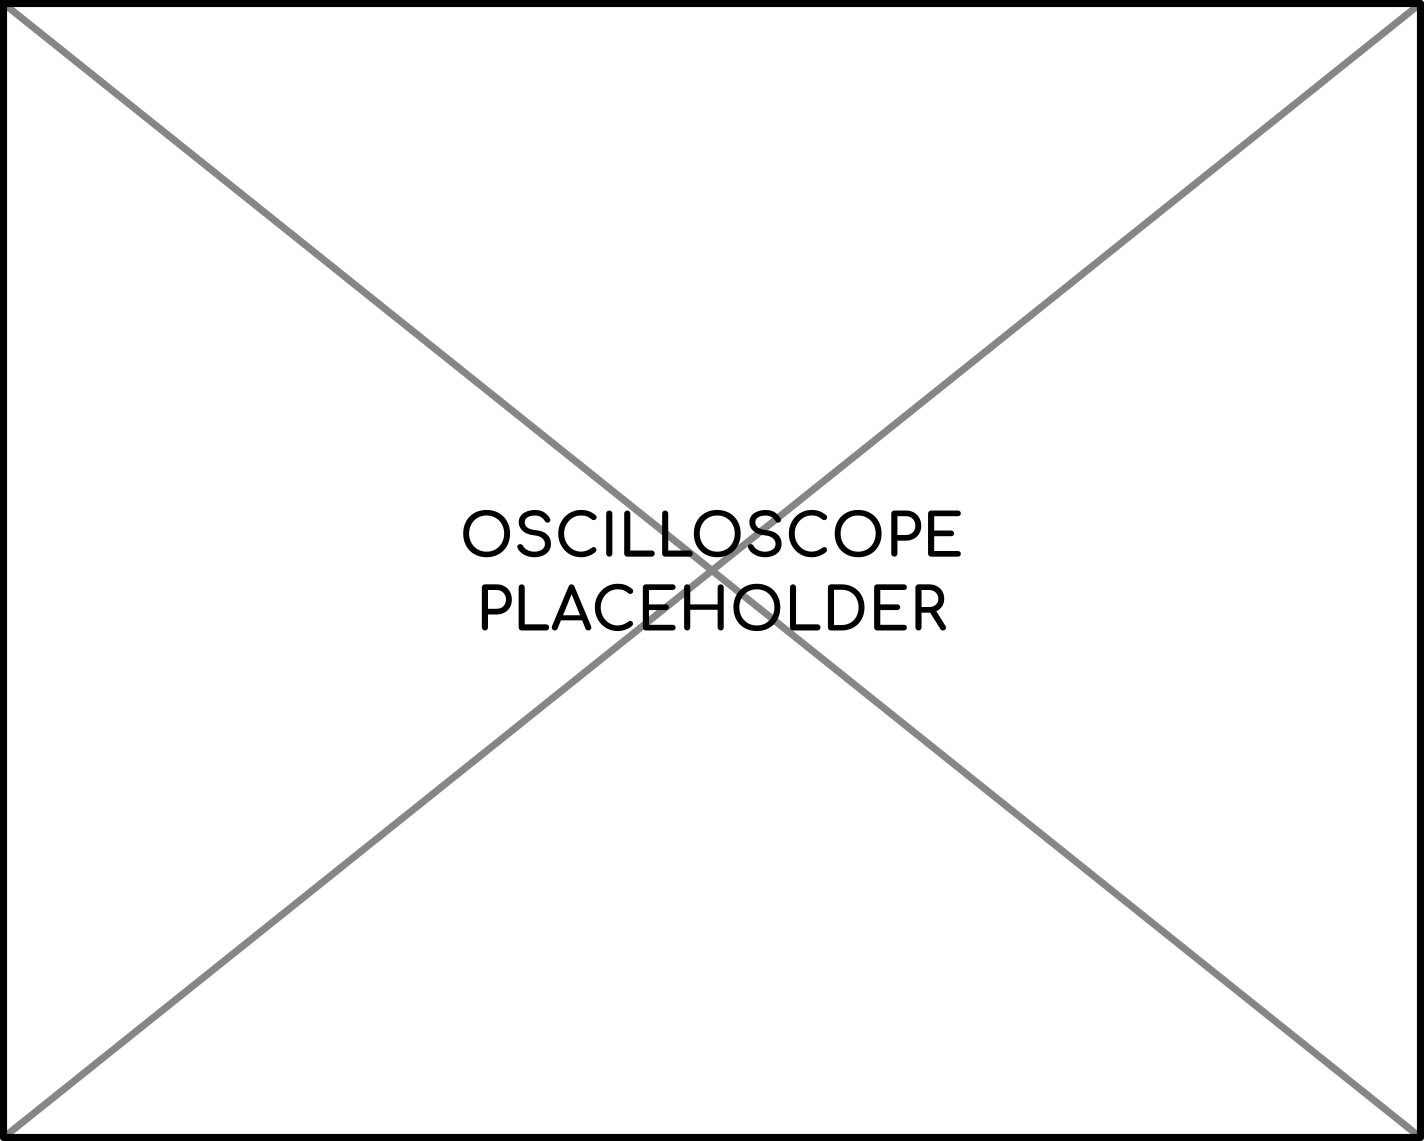
\includegraphics{misc/oscilloscope_placeholder.png}
        \caption{Acquisizione dei segnali $f_{clk}$ e ½$f_{clk}$}
        \label{acq_clock_divider}
    \end{subfigure}

    \caption{Correttezza del circuito divisore di frequenza}
    \label{clock_divider}
\end{figure}

\begin{figure}[H]
    \centering

    \begin{subfigure}{.5\textwidth}
        \centering
        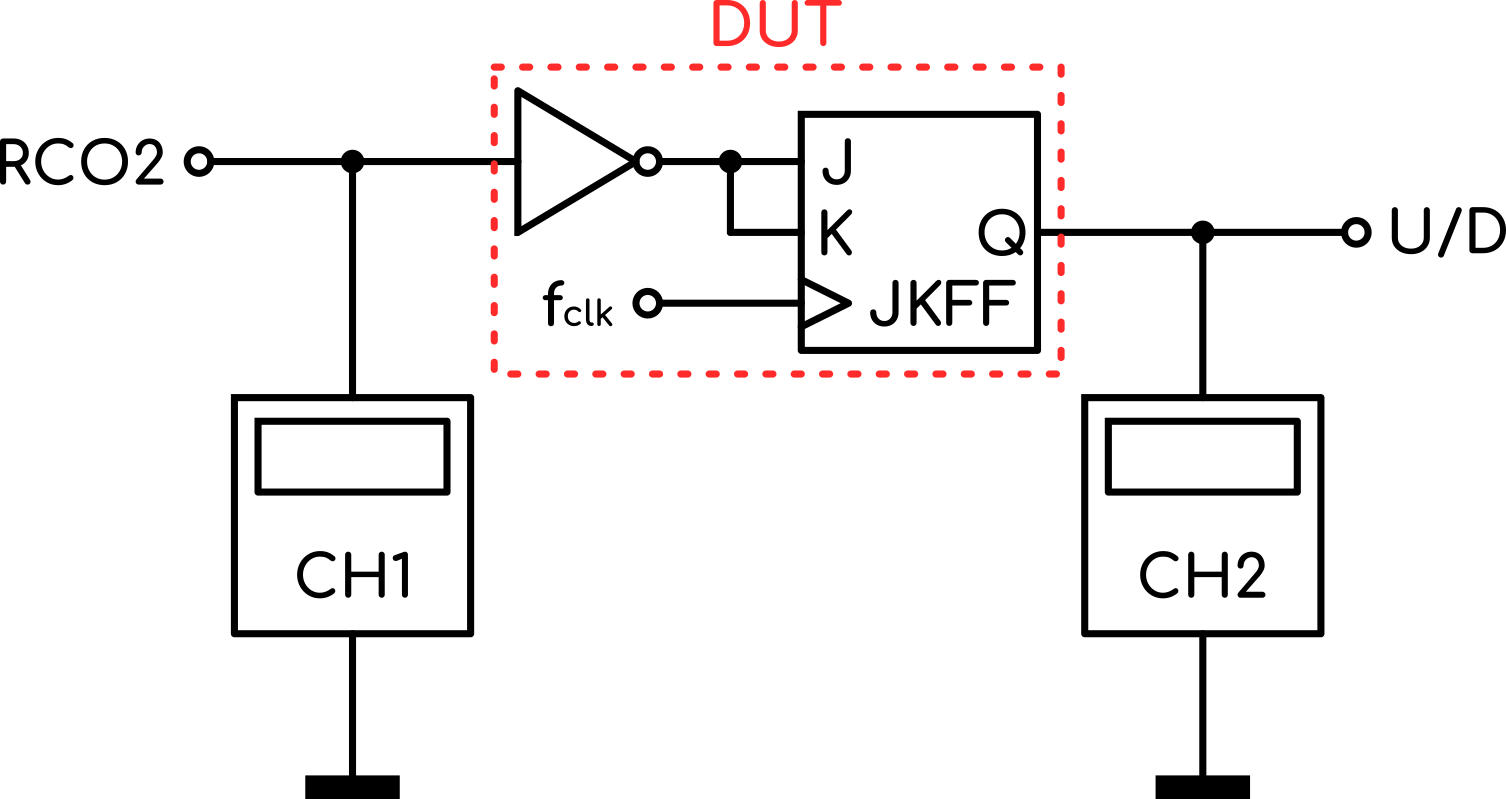
\includegraphics{block_diagrams/mis_UD.png}
        \caption{Circuito di misura del segnale $U/D$}
        \label{mis_UD}
    \end{subfigure}%
    \begin{subfigure}{.5\textwidth}
        \centering
        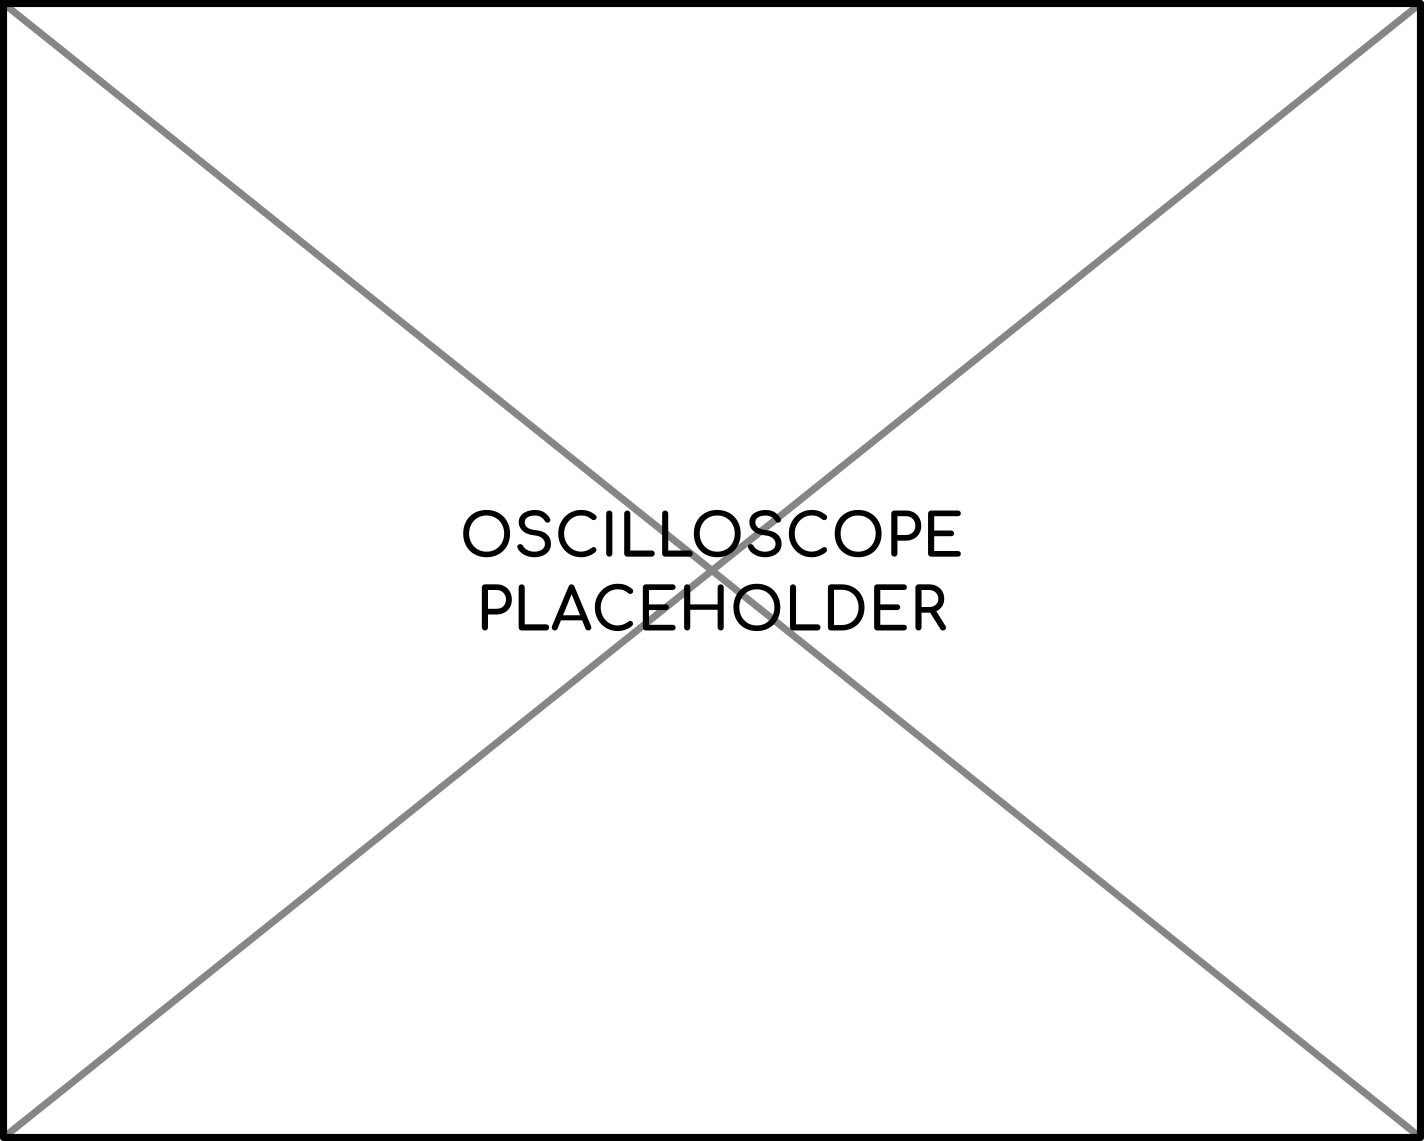
\includegraphics{misc/oscilloscope_placeholder.png}
        \caption{Acquisizione dei segnali $RCO2$ e $U/D$}
        \label{acq_UD}
    \end{subfigure}

    \caption{Correttezza del circuito di pilotaggio del contatore up-down}
    \label{UD}
\end{figure}

%--------------------------------------------------------------------------------------------

\chapter{Convertitore Tensione-Frequenza}

%--------------------------------------------------------------------------------------------

Si vuole ora progettare il circuito per la generazione del segnale $f_{clk}$, con le
specifiche ottenute dai capitoli precedenti, ovvero:

\begin{itemize}
    \item Frequenza minima: $\approx 14\ kHz$;
    \item Frequenza massima: $\approx 3.6\ MHz$;
    \item Livello logico basso: $0\ V$;
    \item Livello logico alto: $+5\ V$;
\end{itemize}

%--------------------------------------------------------------------------------------------

\subsection*{Principio di Funzionamento}

%--------------------------------------------------------------------------------------------

Ciò di cui abbiamo bisogno è un circuito in grado di convertire una tensione in un segnale
a onda rettangolare con frequenza proporzionale alla tensione stessa, ovvero un convertitore
tensione-frequenza.

In commercio è possibile trovare diversi chip in grado di svolgere questa funzione
semplicemente aggiungendo una manciata di componenti di contorno, anche se la maggior
parte di questi non arriva a coprire l'intero range di funzionamento di cui abbiamo bisogno
(come ad esempio il noto LM331 \cite{lm331}). Nel nostro caso si utilizza un VFC110
\cite{vfc110}, circuito integrato specializzato che vanta un'ottima linearità e la capacità
di fornire una frequenza massima di $4\ MHz$ in uscita con una corrispondente tensione in
ingresso di $+10\ V$, esattamente ciò che la nostra applicazione richiede.

\begin{figure}[H]
    \centering
    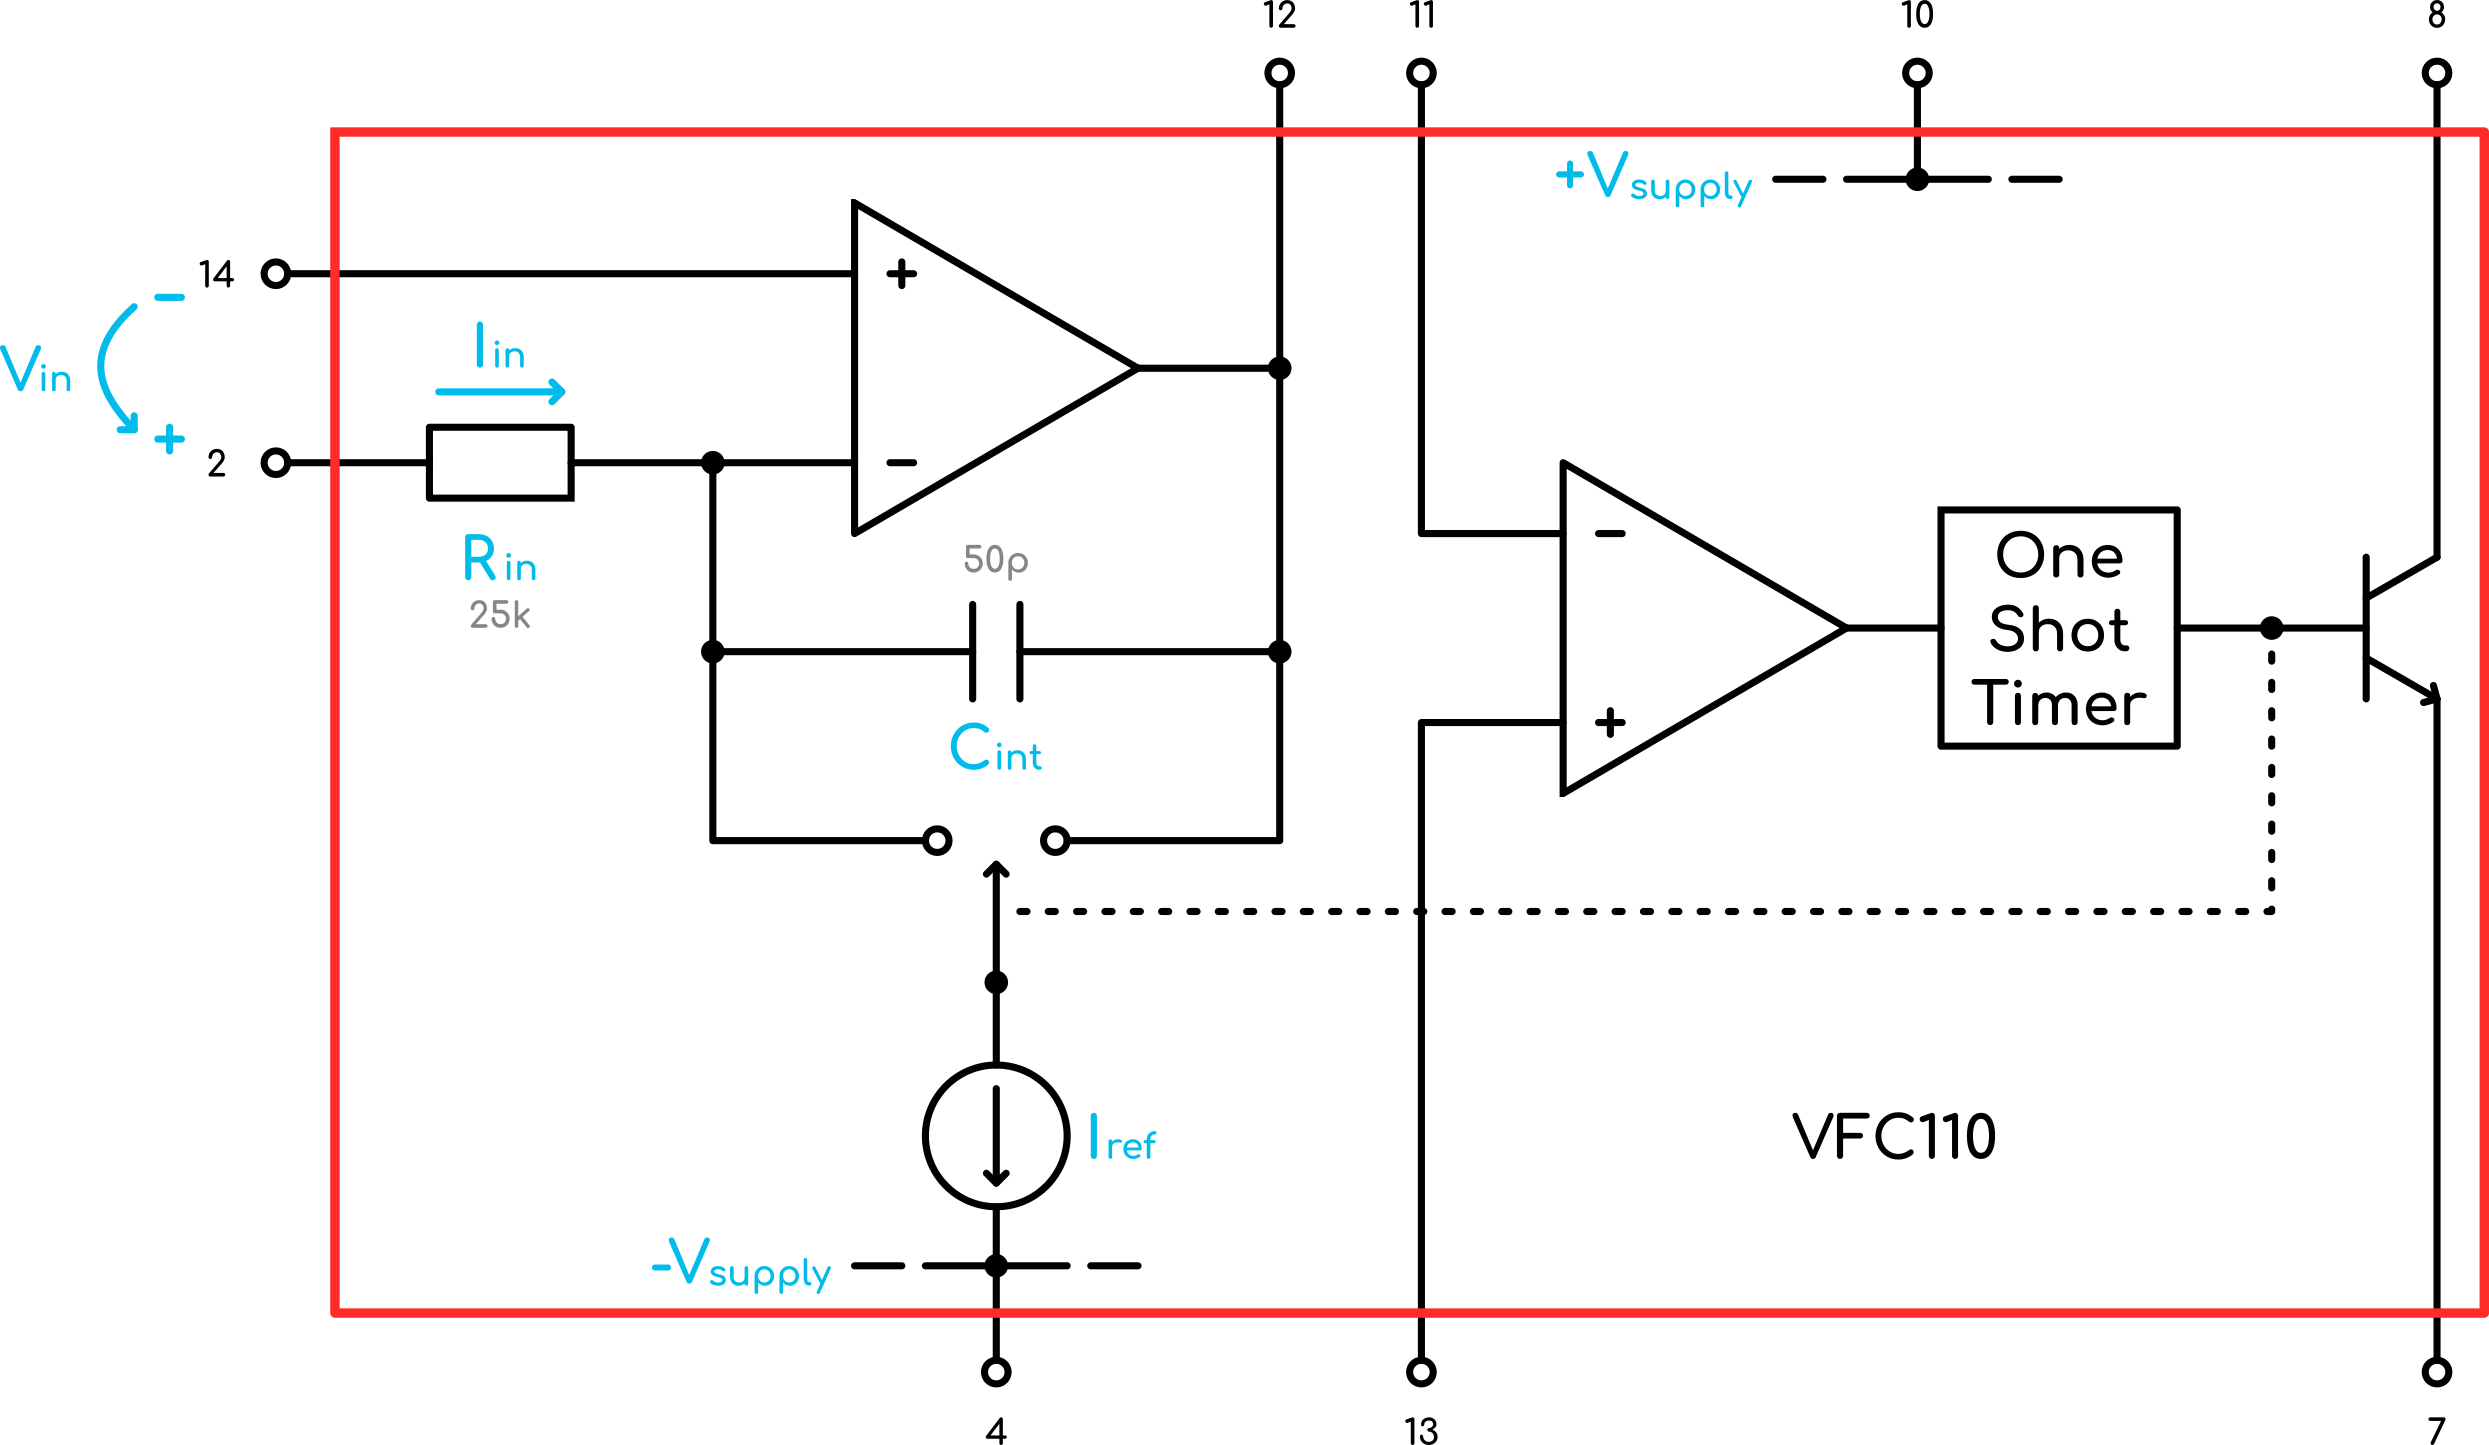
\includegraphics{circuits/vfc110_internal.png}
    \caption{Estratto utile della struttura interna di un VFC110}
    \label{vfc110_internal}
\end{figure}

Il cuore del circuito (figura \ref{vfc110_internal}) consiste in un operazionale configurato
come integratore, con tensione di uscita proporzionale alla carica immagazzinata nella sua
capacità di feedback $C_{int}$. Una tensione in ingresso $V_{in}$ sviluppa una corrente
$I_{in}=\frac{V_{in}}{R_{in}}$ che viene forzata in $C_{int}$, causando quindi una rampa
decrescente in uscita. Arrivati a $0\ V$ il comparatore scatta, attivando il timer one-shot.
Quindi un generatore di corrente $I_{ref}$ (dal valore di circa $1\ mA$) viene connesso
all'ingresso dell'integratore per un periodo di durata pari a $T_{OS}$, causando una rampa
crescente in uscita. Infine il ciclo ricomincia.

\begin{figure}[H]
    \centering
    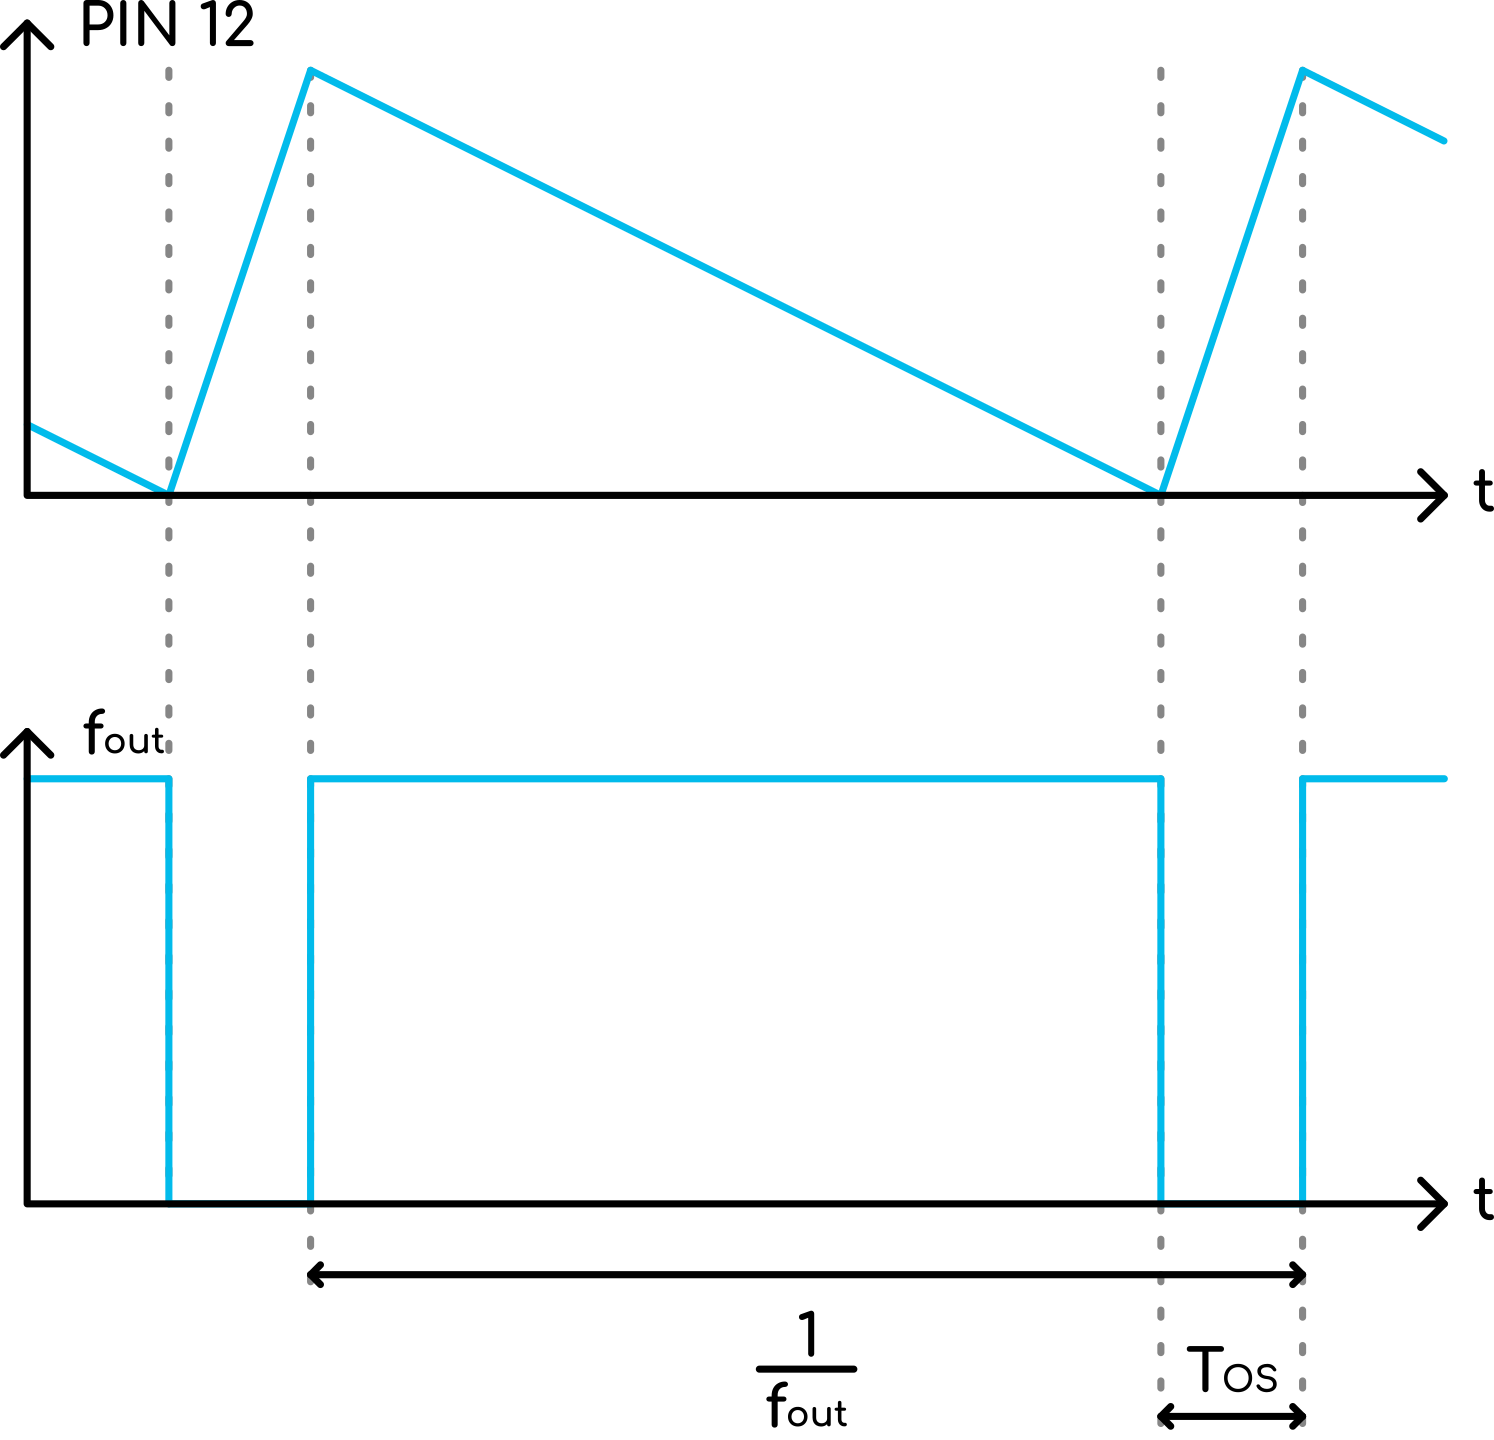
\includegraphics{graphs/integrator_behaviour.png}
    \caption{Forme d'onda teoriche del VFC110}
    \label{integrator_behaviour}
\end{figure}

Per uno studio più approfondito sul funzionamento del VFC110 si consiglia la lettura del
datasheet del componente, dal quale si ricava la configurazione del circuito utilizzato
per sfruttare l'intero range offerto (figura \ref{VFC_circuit}). Si modificano solo i valori
di alimentazione, sostituendoli con quelli dello standard scelto.

\begin{figure}[H]
    \centering
    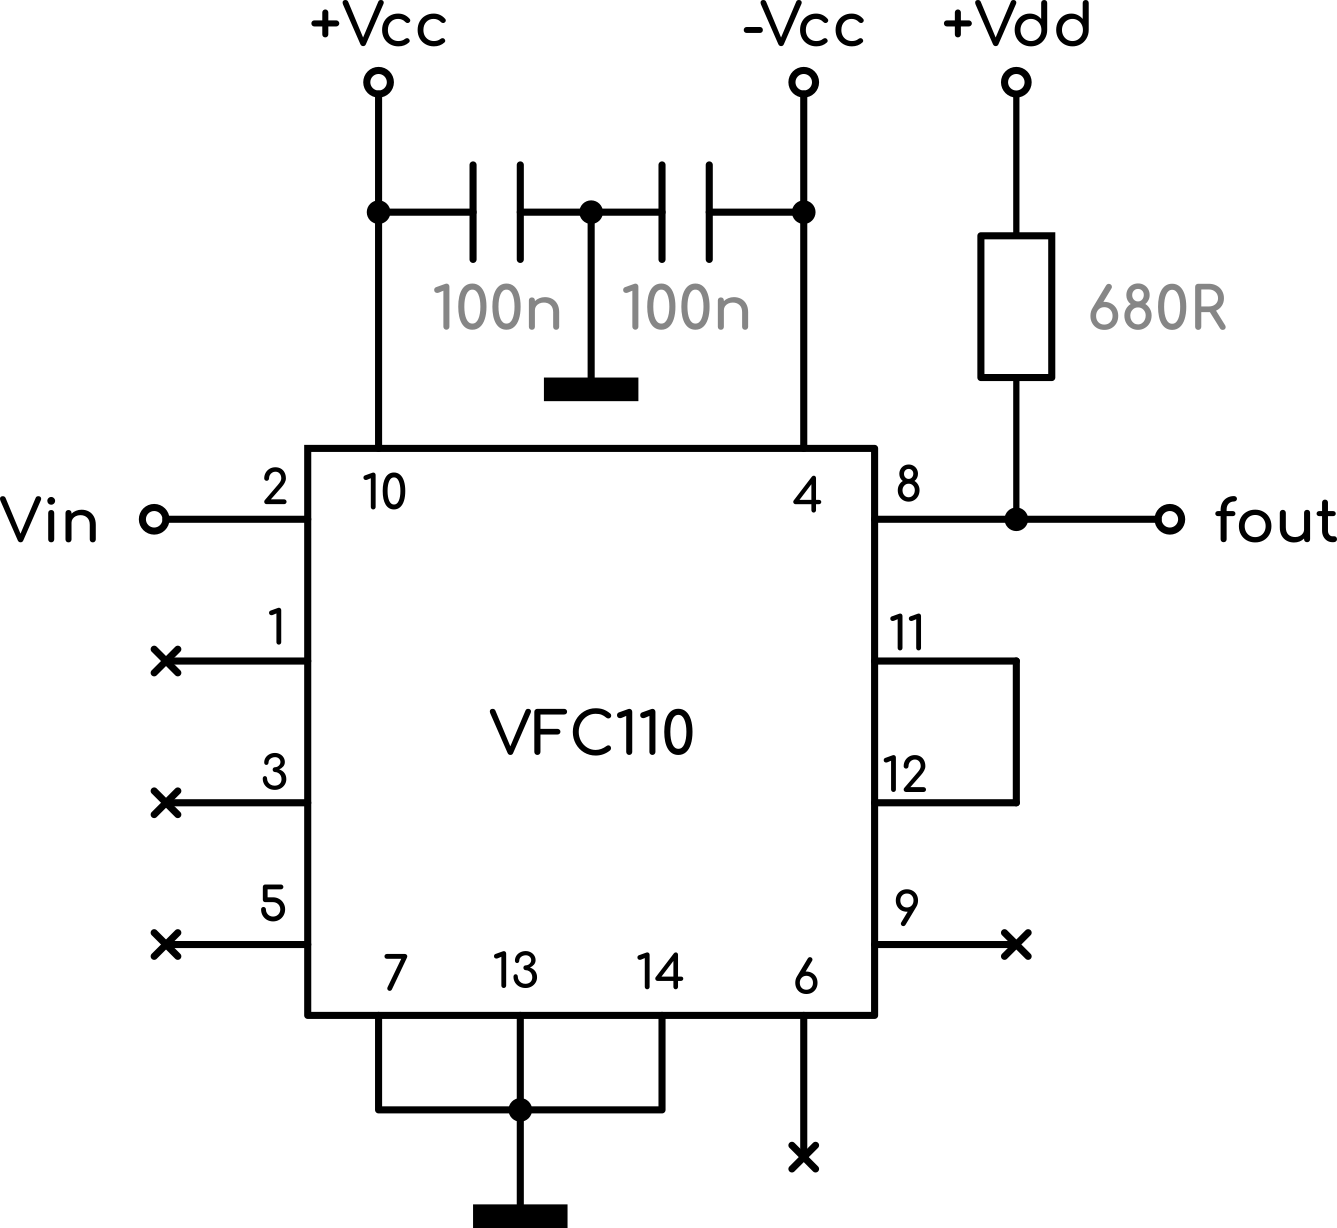
\includegraphics{circuits/VFC_circuit.png}
    \caption{Schema elettrico del circuito utilizzato ($\pm V_{cc}=\pm 12\ V$, $+V_{}=+5\ V$)}
    \label{VFC_circuit}
\end{figure}

Si noti che gli unici componenti aggiunti sono condensatori di filtro e un resistore di
pull-up per l'uscita a collettore aperto.

Si riportano anche le relazioni tra le principali grandezze in gioco:

\begin{equation}\label{duty_cycle}
    I_{in}=I_{ref}\cdot\delta\ [A]
    \qquad
    \rightarrow
    \qquad
    \delta=\frac{I_{in}}{I_{ref}}=\frac{V_{in}}{R_{in}\cdot I_{ref}}
\end{equation}

\begin{equation}\label{fout}
    \frac{V_{in}}{R_{in}}=I_{ref}\cdot f_{out}\cdot T_{OS}\ [A]
    \qquad
    \rightarrow
    \qquad
    f_{out}=\frac{V_{in}}{R_{in}\cdot I_{ref}\cdot T_{OS}}=\frac{\delta}{T_{OS}}\ [Hz]
\end{equation}

%--------------------------------------------------------------------------------------------

\subsection*{Risultati Pratici e Misure}

%--------------------------------------------------------------------------------------------

Si procede quindi alla verifica del corretto funzionamento del circuito. Il setup di
misura utilizzato è il seguente:

\begin{figure}[H]
    \centering
    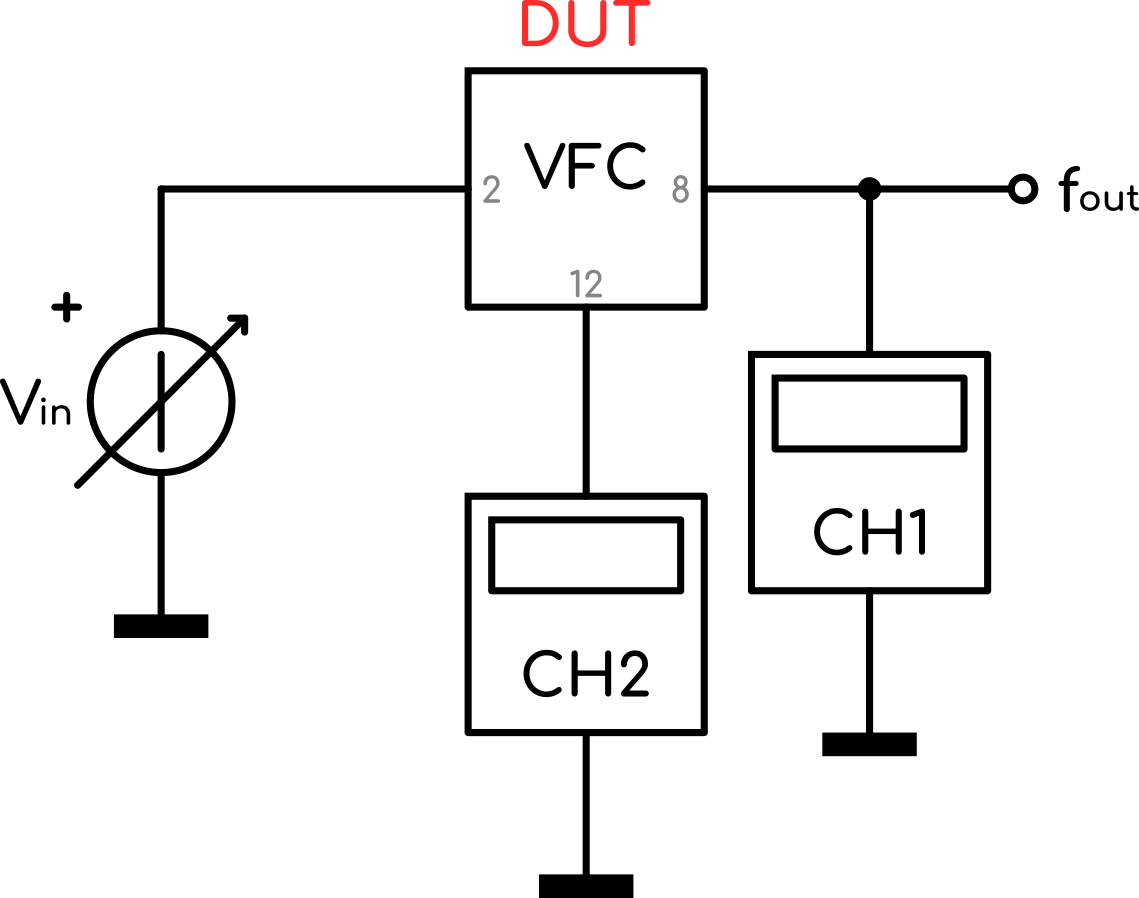
\includegraphics{block_diagrams/mis_VFC.png}
    \caption{Setup di misura del VFC}
    \label{mis_VFC}
\end{figure}

Successivamente si raccolgono in tabella i dati che verranno poi utilizzati per tracciare i
grafici corrispondenti:

\begin{table}[H]
    \centering
    \csvreader[
    tabular = |C||C|L|,
    table head = {\hline \rowcolor{myLightGrey} $V_{in}\ [V]$ & $\delta\ [\%]$ & $f_{out}\ [kHz]$ \\\hline},
    late after line = \\\hline,
    ]{data/misure_vfc.csv}{}{
    \csvcoli & \csvcoliii & \csvcolv
    }
    \caption{Valori misurati del blocco VFC}
    \label{vfc_table}
\end{table}

Possiamo anzitutto verificare che il comportamento dell'integratore corrisponde a quello
descritto nel paragrafo precedente, e si nota che la durata del periodo basso di $f_{out}$
si estende lungo il tratto di rampa crescente come in figura \ref{integrator_behaviour},
ovvero durante il periodo $T_{OS}$, in cui il timer risulta attivo. Possiamo anche
notare che la sua durata non varia in funzione di $V_{in}$ o $f_{out}$, ma rimane invece
pressoché costante a circa $100\ ns$. Questo valore risulta corretto se inserito nella
formula \ref{fout} poichè fornisce una stima accurata dei valori di frequenza misurati.

\begin{figure}[H]
    \centering

    \begin{subfigure}{.5\textwidth}
        \centering
        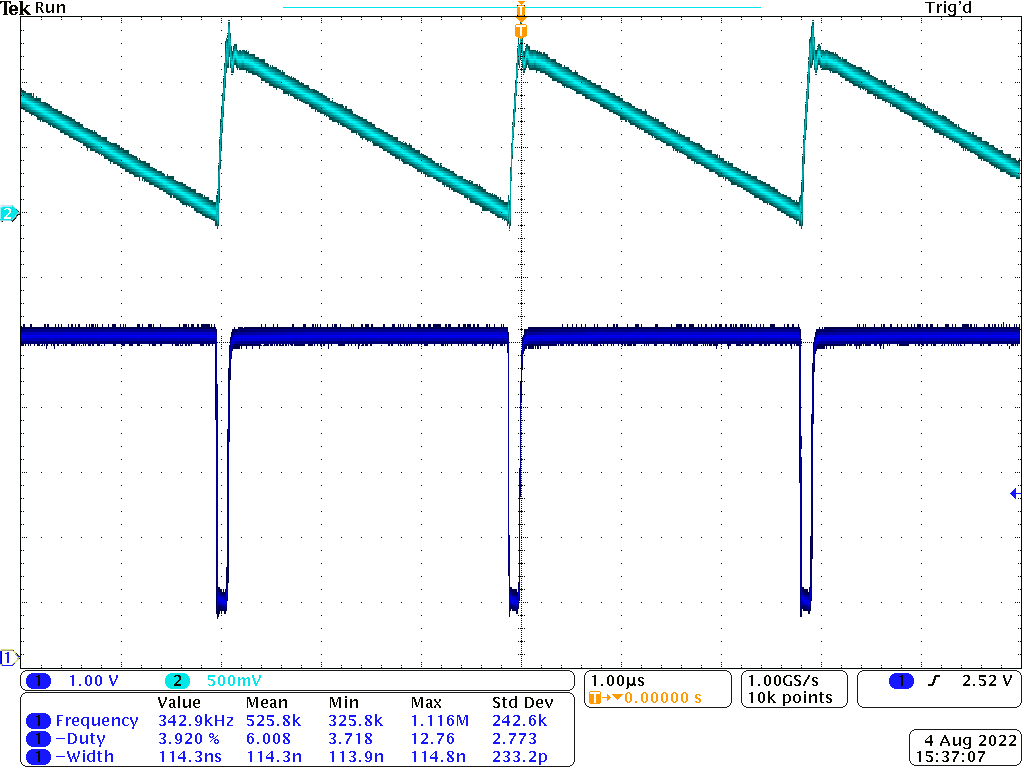
\includegraphics[scale = 0.2]{acquisitions/VFC_1V.png}
        \caption{$V_{in}=1\ V$}
        \label{acq_vfc110_1v}
    \end{subfigure}%
    \begin{subfigure}{.5\textwidth}
        \centering
        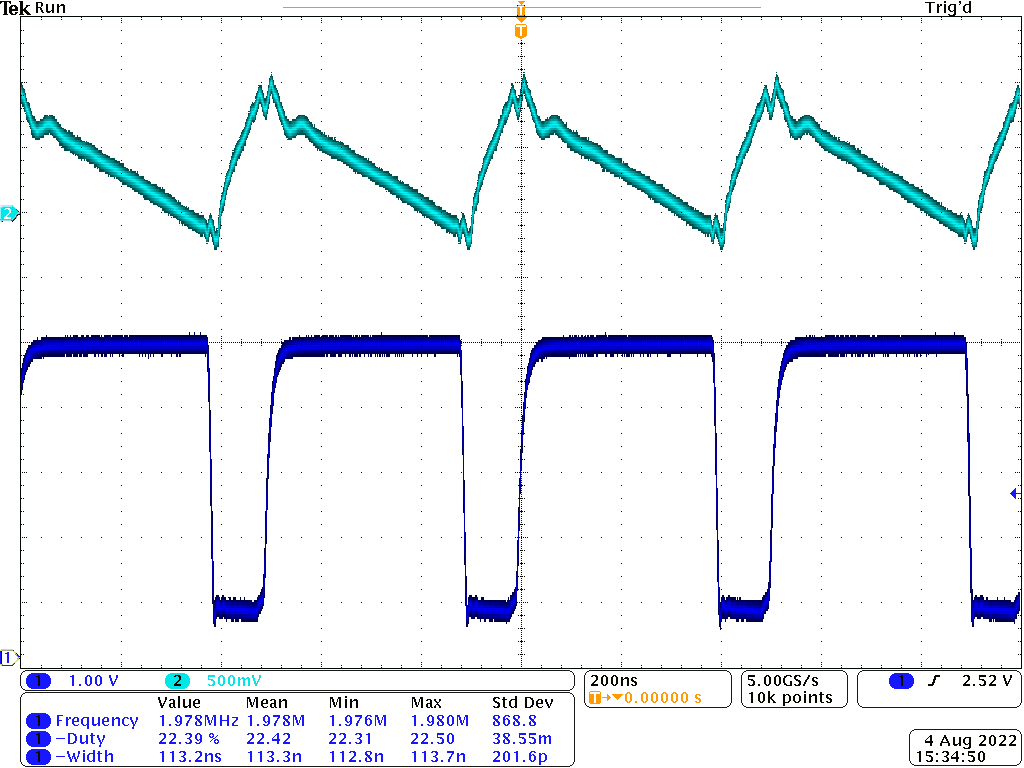
\includegraphics[scale = 0.2]{acquisitions/VFC_5V.png}
        \caption{$V_{in}=5\ V$}
        \label{acq_vfc110_5v}
    \end{subfigure}
    \begin{subfigure}{.5\textwidth}
        \centering
        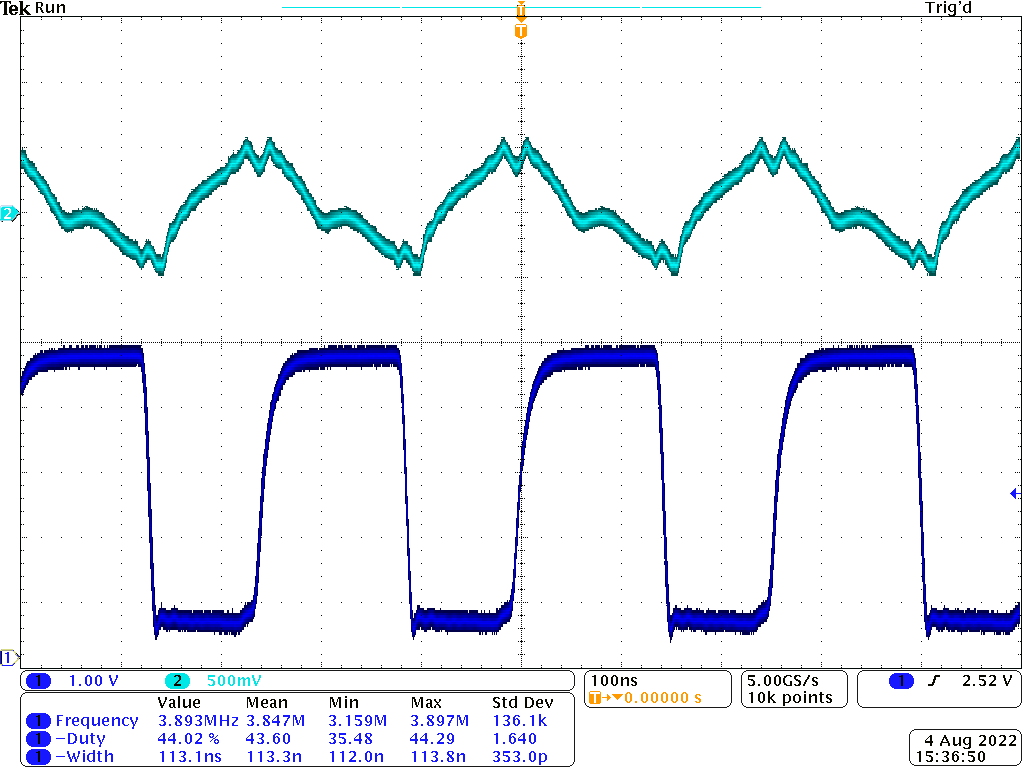
\includegraphics[scale = 0.2]{acquisitions/VFC_10V.png}
        \caption{$V_{in}=10\ V$}
        \label{acq_vfc110_10v}
    \end{subfigure}

    \caption{Acquisizioni dei segnali di interesse per diversi valori di $V_{in}$}
    \label{acq_vfc110}
\end{figure}

\begin{figure}[H]
    \centering

    \begin{subfigure}{.5\textwidth}
        \centering
        \begin{tikzpicture}[scale = 0.85]
            \begin{axis}[
                    title = Duty Cycle,             % title
                    no marks,
                    xmin = 0, xmax = 12,            % limit values
                    ymin = 0, ymax = 50,
                    grid = major,                   % grid
                    grid style = {dashed, gray!30},
                    xlabel = $V_{in}$,              % axis titles and units
                    ylabel = $\delta$,
                    x unit = \si{\V}, y unit = \si{\percent},
                    legend style = {at = {(0.5, -0.25)}, anchor = north},
                    cycle list name = modular,
                ]

                \addplot
                table[x = vin, y = duty atteso, col sep = comma]{./data/misure_vfc.csv};

                \addplot
                table[x = vin, y = duty misurato, col sep = comma]{./data/misure_vfc.csv};

                \legend{Formula \ref{duty_cycle}, Valori misurati}
            \end{axis}
        \end{tikzpicture}
    \end{subfigure}%
    \begin{subfigure}{.5\textwidth}
        \centering
        \begin{tikzpicture}[scale = 0.85]
            \begin{axis}[
                    title = Frequenza,              % title
                    no marks,
                    xmin = 0, xmax = 12,            % limit values
                    ymin = 0, ymax = 5000,
                    grid = major,                   % grid
                    grid style = {dashed, gray!30},
                    xlabel = $V_{in}$,              % axis titles and units
                    ylabel = $f_{out}$,
                    x unit = \si{\V}, y unit = \si{\kHz},
                    legend style = {at = {(0.5, -0.25)}, anchor = north},
                    cycle list name = modular,
                ]

                \addplot
                table[x = vin, y = fout attesa, col sep = comma]{./data/misure_vfc.csv};

                \addplot
                table[x = vin, y = fout misurata, col sep = comma]{./data/misure_vfc.csv};

                \legend{Formula \ref{fout}, Valori misurati}
            \end{axis}
        \end{tikzpicture}
    \end{subfigure}

    \caption{Grafici delle grandezze riportate in tabella \ref{vfc_table}}
    \label{vfc_graphs}
\end{figure}

Si nota che l'andamento del duty cycle si distacca leggermente dalla teoria, pur avendo
comunque un comportamento lineare. Questo è dovuto probabilmente a causa di diverse
non-idealità del componente, come ad esempio le tolleranze dei componenti interni al
VFC110, tuttavia il parametro di maggiore interesse in questo caso è $f_{out}$, che invece
risulta quasi uguale ai valori calcolati, come evidente in figura \ref{vfc_graphs}b.

%--------------------------------------------------------------------------------------------

\chapter{Condizionamento dell'Ingresso}

%--------------------------------------------------------------------------------------------

\section{Convertitore Lineare-Esponenziale}

%--------------------------------------------------------------------------------------------

Vogliamo ora analizzare il circuto che soddisfa la specifica sulla modalità $1V/Octave$
dell'ingresso, ovvero il circuito in grado di convertire una tensione lineare in una
esponenziale.

Il circuito utilizzato è molto diffuso in questo tipo di applicazioni, si può infatti
trovare in molti siti di DIY come quello di René Schmitz \cite{expo_converter}, personaggio
molto noto tra gli appassionati di sintetizzatori musicali fai-da-te.

%--------------------------------------------------------------------------------------------

\subsection*{Analisi del Circuito}

%--------------------------------------------------------------------------------------------

Per l'applicazione si sfrutta la caratteristica esponenziale intrinseca del transistor
bipolare:

\begin{displaymath}
    I_e\approx I_c=I_se^{\left(\frac{V_{be}}{V_T}-1\right)}
    \approx I_se^{\left(\frac{V_{be}}{V_T}\right)}\ [A]
\end{displaymath}

\begin{figure}[H]
    \centering
    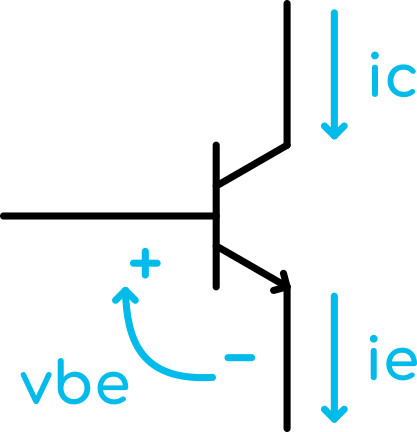
\includegraphics{circuits/single_transistor_circuit.png}
    \caption{BJT}
    \label{bjt}
\end{figure}

dove $V_T$ (o potenziale termico) e $I_s$ (o corrente di saturazione) sono variabili in
funzione della temperatura, anche se nella nostra analisi $V_T$ verrà considerato di
valore costante pari a $26\ mV$.

Per rimuovere dall'equazione $I_s$, che invece risulta molto più problematico, si collega
una coppia di transistor (idealmente nello stesso chip, in modo che siano il più possibile
simili tra loro e termicamente accoppiati) in configurazione differenziale:

\begin{figure}[H]
    \centering
    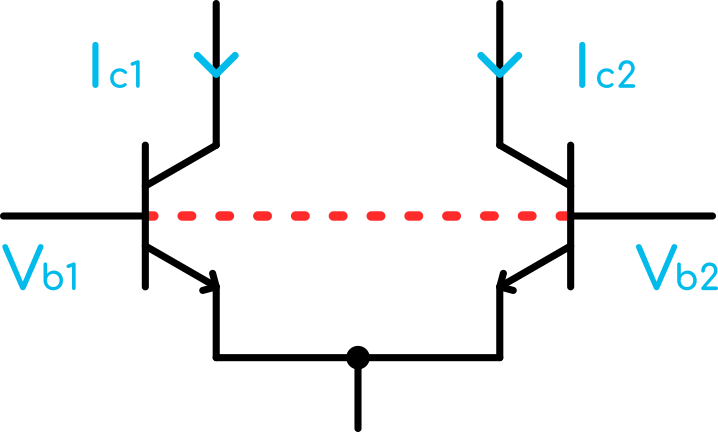
\includegraphics{circuits/differential_pair_circuit.png}
    \caption{Coppia differenziale a BJT}
    \label{differential_pair_circuit}
\end{figure}

per la quale possiamo scrivere la seguente relazione:

\begin{displaymath}
    \frac{I_{c2}}{I_{c1}}=\frac{I_s e^{\left(\frac{V_{be2}}{V_T}\right)}}{I_s e^{\left(\frac{V_{be1}}{V_T}\right)}}
    \qquad
    \rightarrow
    \qquad
    I_{c2}=I_{c1}e^{\left(\frac{V_{be2}-V_{be1}}{V_T}\right)}=I_{c1}e^{\left(\frac{V_{b2}-V_{b1}}{V_T}\right)}\ [A]
\end{displaymath}

in cui risulta evidente che la dipendenza da $I_s$ viene completamente rimossa.

A questo punto, rinominiamo le grandezze come segue:

\begin{displaymath}
    I_{freq}=I_{ref}e^{\left(-\frac{V_{b1}}{V_T}\right)}\ [A]
\end{displaymath}

e aggiungiamo al circuito

\begin{itemize}
    \item un amplificatore per portare $V_{in}$ in un range appropriato alla base di $Q_1$
          (operazionale di sinistra, figura \ref{exponential_converter_circuit})
          \begin{displaymath}
              V_{b1}=-V_{in}\cdot s=
              -V_{in}\cdot\frac{R_f}{R_{in}}\cdot\frac{\%R_{pot}+R}{R_{pot}+R}\ [V]
          \end{displaymath}
    \item un anello di controllo per mantenere la corrente di riferimento $I_{ref}$ costante
          (operazionale centrale, figura \ref{exponential_converter_circuit})
          \begin{displaymath}
              I_{ref}=\frac{V_{HR}-V_{LR}}{R_{ref}}\ [A]
          \end{displaymath}
    \item un convertitore corrente-tensione al collettore di $Q_2$ (operazionale di destra,
          figura \ref{exponential_converter_circuit})
          \begin{displaymath}
              V_{exp}=-I_{freq}\cdot R_{conv}\ [V]
          \end{displaymath}
\end{itemize}

ottenendo quindi il seguente circuito con la relativa relazione ingresso/uscita:

\begin{figure}[H]
    \centering
    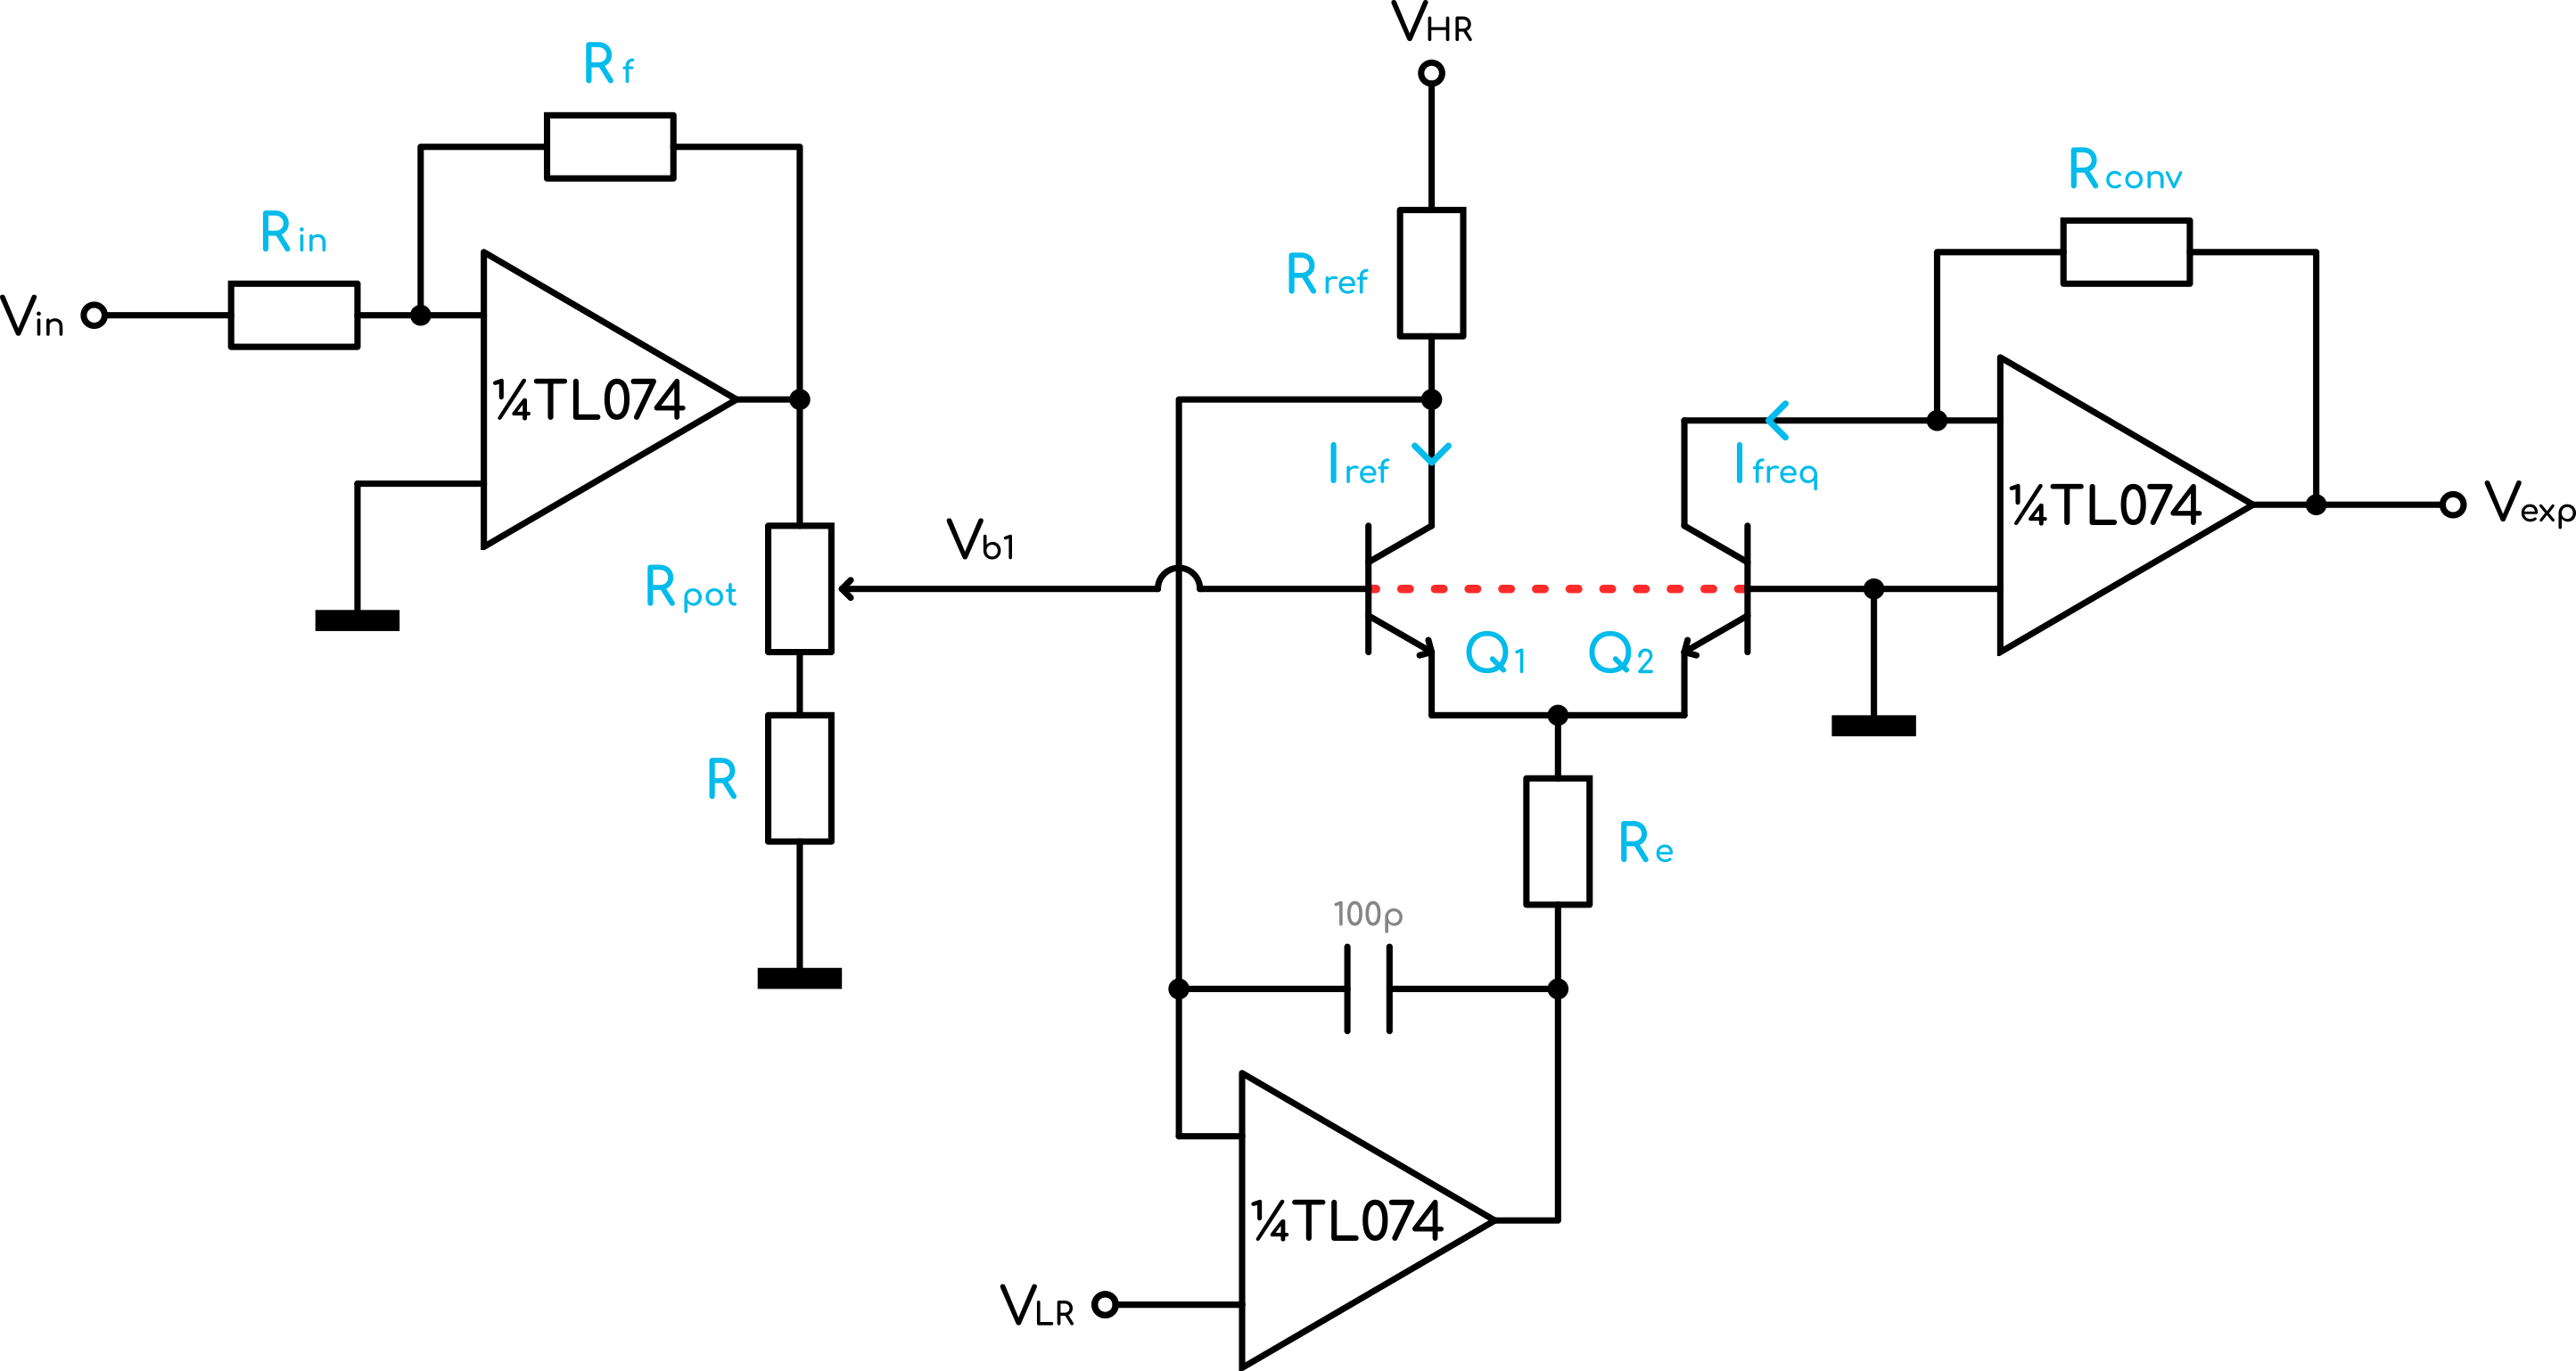
\includegraphics{circuits/exponential_converter_circuit.png}
    \caption{Schema elettrico del convertitore tensione lineare-esponenziale}
    \label{exponential_converter_circuit}
\end{figure}

\begin{displaymath}
    V_{exp}=R_f\cdot \frac{V_{HR}-V_{LR}}{R_{ref}}e^{\left(\frac{s\cdot V_{in}}{V_T}\right)}
\end{displaymath}

%--------------------------------------------------------------------------------------------

\subsection*{Dimensionamento e Scelta dei Componenti}

%--------------------------------------------------------------------------------------------

Passiamo quindi al dimensionamento dei componenti, in modo da imporre al circuito il
comportamento voluto.

Come prima cosa calcoliamo il valore del guadagno $s$ dell'amplificatore invertente.
Si vuole:

\begin{displaymath}
    I_{freq}=I_{ref}e^{\left(\frac{s\cdot V_{in}}{V_T}\right)}
    \qquad
    \rightarrow
    \qquad
    2I_{freq}=I_{ref}e^{\left(\frac{s\cdot(V_{in}+\Delta V_{in})}{V_T}\right)}
\end{displaymath}

qundi un raddoppio della corrente $I_{freq}$ per ogni variazione $\Delta V_{in}=1\ V$.
Allora possiamo riscrivere le due relazioni nel seguente modo:

\begin{displaymath}
    2=e^{\left(\frac{s\cdot\Delta V_{in}}{V_T}\right)}
    \qquad
    \rightarrow
    \qquad
    ln(2)=\frac{s\cdot\Delta V_{in}}{V_T}
    \qquad
    \rightarrow
    \qquad
    s=\frac{V_T\cdot ln(2)}{\Delta V_{in}}
\end{displaymath}

\begin{displaymath}
    s=\frac{26\ mV\cdot 0.6931}{1\ V}\approx0.018\approx\frac{1}{55.5}
\end{displaymath}

\begin{displaymath}
    s=\frac{R_f}{R_{in}}\cdot\frac{\%R_{pot}+R}{R_{pot}+R}
    =\frac{2\ k\Omega}{100\ k\Omega}\cdot\frac{440\ \Omega}{490\ \Omega}
    \approx 0.018
\end{displaymath}

quindi:

\begin{itemize}
    \item $R_f = 2\ k\Omega$;
    \item $R_{in} = 100\ k\Omega$;
    \item $R_{pot} = 100\ \Omega$;
    \item $R = 390\ \Omega$;
\end{itemize}

Scegliamo anche $R_{conv}=3.3\ k\Omega$, per avere come massimo valore di corrente
$I_{freq} = 3\ mA$ ($\approx+10\ V$ in uscita dal convertitore corrente-tensione),
in corrispondenza di una tensione di ingresso di $+8\ V$. Da qui possiamo quindi calcolare
il valore di $I_{ref}$:

\begin{displaymath}
    I_{ref}=I_{freq}e^{\left(-\frac{s\cdot V_{in}}{V_T}\right)}
    =0.003e^{\left(-\frac{0.018\cdot8}{0.026}\right)}
    \approx11.8\ \mu A
\end{displaymath}

Impostando quindi $V_{HR}=+12\ V$ e $V_{LR}=0\ V$ calcoliamo $R_{ref}$:

\begin{displaymath}
    R_{ref}=\frac{V_{HR}}{I_{ref}}=\frac{12}{11.8\cdot10^{-6}}\approx 1\ M\Omega
\end{displaymath}

Ora, poichè la corrente massima a scorrere in $R_e$ è la somma di $I_{ref}$ e $I_{freq}$
e quindi $\approx3\ \mu A$ possiamo scegliere anche $R_e=R_{conv}=3.3\ k\Omega$. In questo
modo sommando le cadute di potenziale $V_{R_{ref}}$, $V_{ce\_sat\_1}$ e $V_{R_e}$, siamo
dentro il limite dei valori di alimentazione, ottenendo $\approx 22.2\ V\ < 24\ V= 2V_{cc}$.

Tuttavia, qualora dovessero presentarsi problemi di saturazione prematura, è possibile
collegare un altro transistor in configurazione a diodo (o più semplicemente un diodo), per
ridurre la corrente che scorre nel ramo di $R_e$ e quindi la tensione ai suoi capi (in modo
non lineare). Il diodo infatti, non appena sufficientemente polarizzato, diventerebbe una
resistenza quasi nulla in parallelo ad una resistenza invece molto maggiore, questo accade
appena $V_{ce2}$ diventa maggiore di $\approx0.7\ V$.

\begin{figure}[H]
    \centering

    \begin{subfigure}{.5\textwidth}
        \centering
        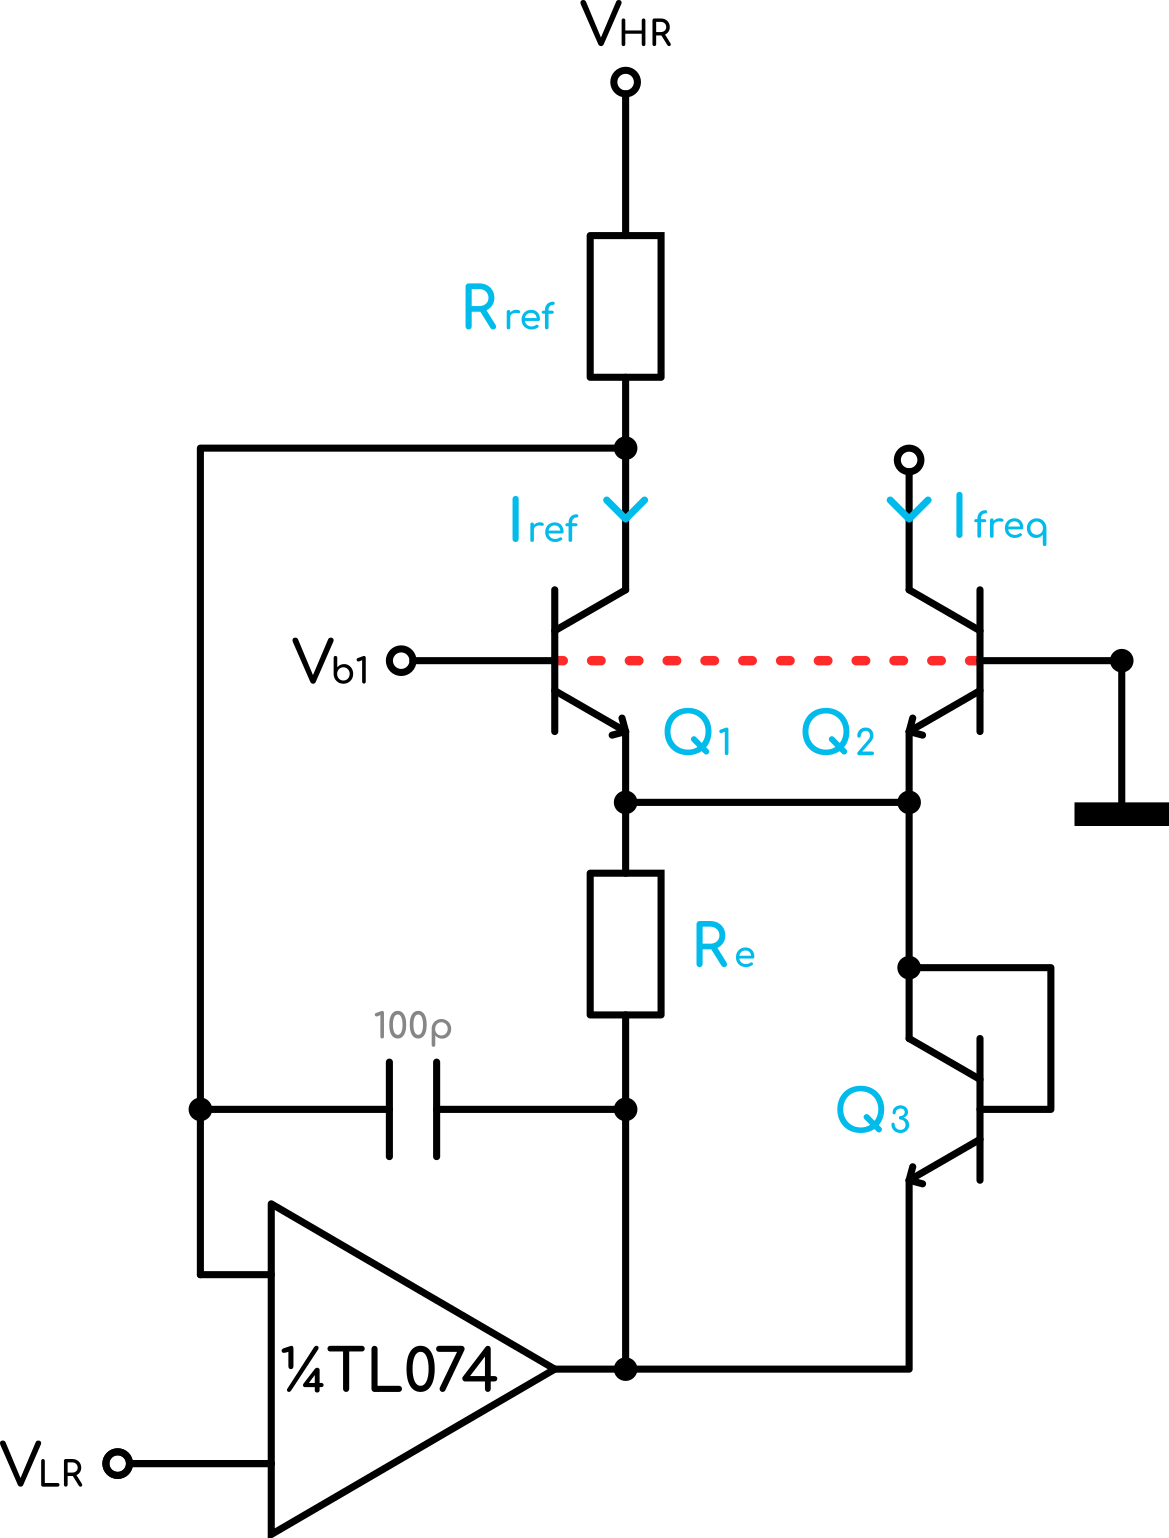
\includegraphics{circuits/expo_converter_transistor_circuit.png}
        \caption{Transistor in configurazione a diodo}
        \label{expo_converter_transistor_circuit}
    \end{subfigure}%
    \begin{subfigure}{.5\textwidth}
        \centering
        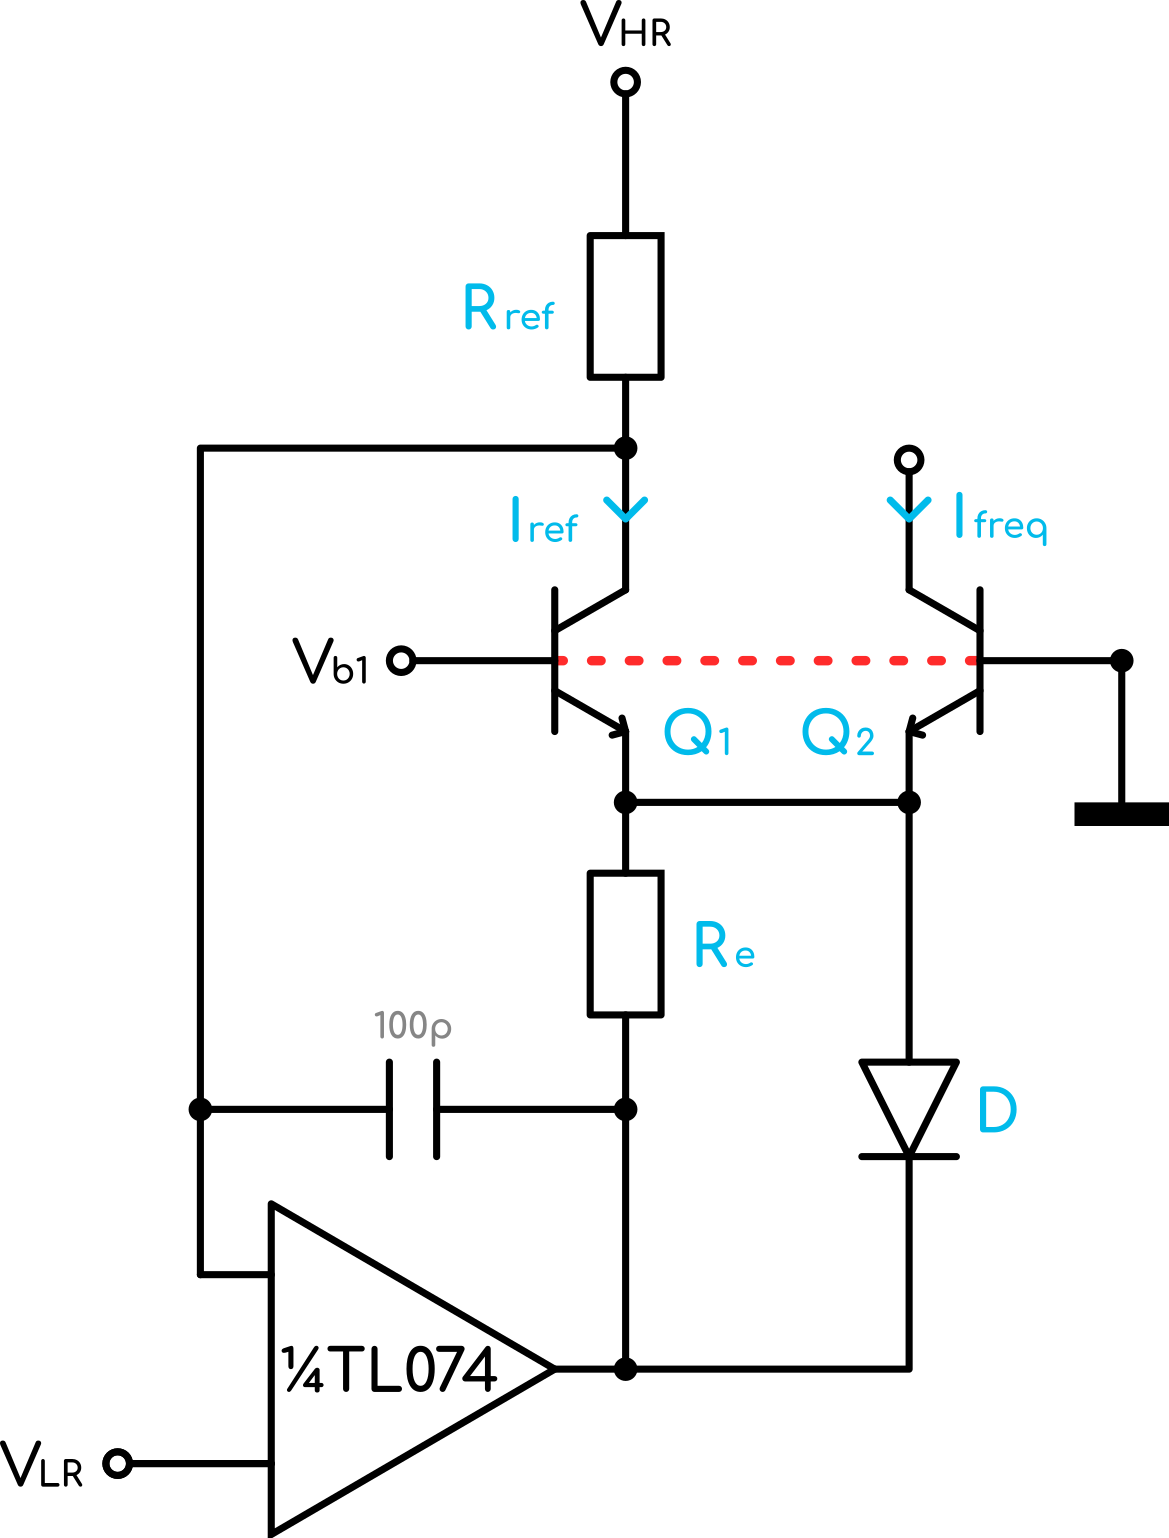
\includegraphics{circuits/expo_converter_diode_circuit.png}
        \caption{Diodo}
        \label{expo_converter_diode_circuit}
    \end{subfigure}

    \caption{Convertitori esponenziali con carico non-lineare}
    \label{non_linear_load_expo}
\end{figure}

Ancora una volta gli amplificatori operazionali utilizzati sono dei TL074, mentre si sceglie
un MPQ3904 \cite{mpq3904} per i transistor, chip che ospita 4 unità al proprio interno.

%--------------------------------------------------------------------------------------------

\subsection*{Risultati Pratici e Misure}

%--------------------------------------------------------------------------------------------

TODO misure e acquisizioni del convertitore lineare-esponenziale

%--------------------------------------------------------------------------------------------

\section{Somma di più Ingressi}

%--------------------------------------------------------------------------------------------

TODO descrizione sommatore

%--------------------------------------------------------------------------------------------

\section{Clipper}

%--------------------------------------------------------------------------------------------

TODO descrizione clipper

%--------------------------------------------------------------------------------------------

\subsection*{Risultati Pratici e Misure}

%--------------------------------------------------------------------------------------------

TODO misure e acquisizioni clipper

%--------------------------------------------------------------------------------------------

\include{chapters/ch04-selezione_modalità.tex}
\chapter{Generazione dei Segnali Secondari}

TODO


\section{Onda Quadra}

TODO


\section{Dente di Sega}

TODO


\section{Sinusoide}

TODO


\section{Impulso}

TODO
\chapter{Stadi di Uscita}

%--------------------------------------------------------------------------------------------

Per quanto rigurarda gli stadi di uscita, si collega in serie un filtro passa-basso attivo,
che avrà anche lo scopo di isolare l'assorbimento di corrente dai circuiti che generano i
segnali.

\begin{figure}[H]
    \centering
    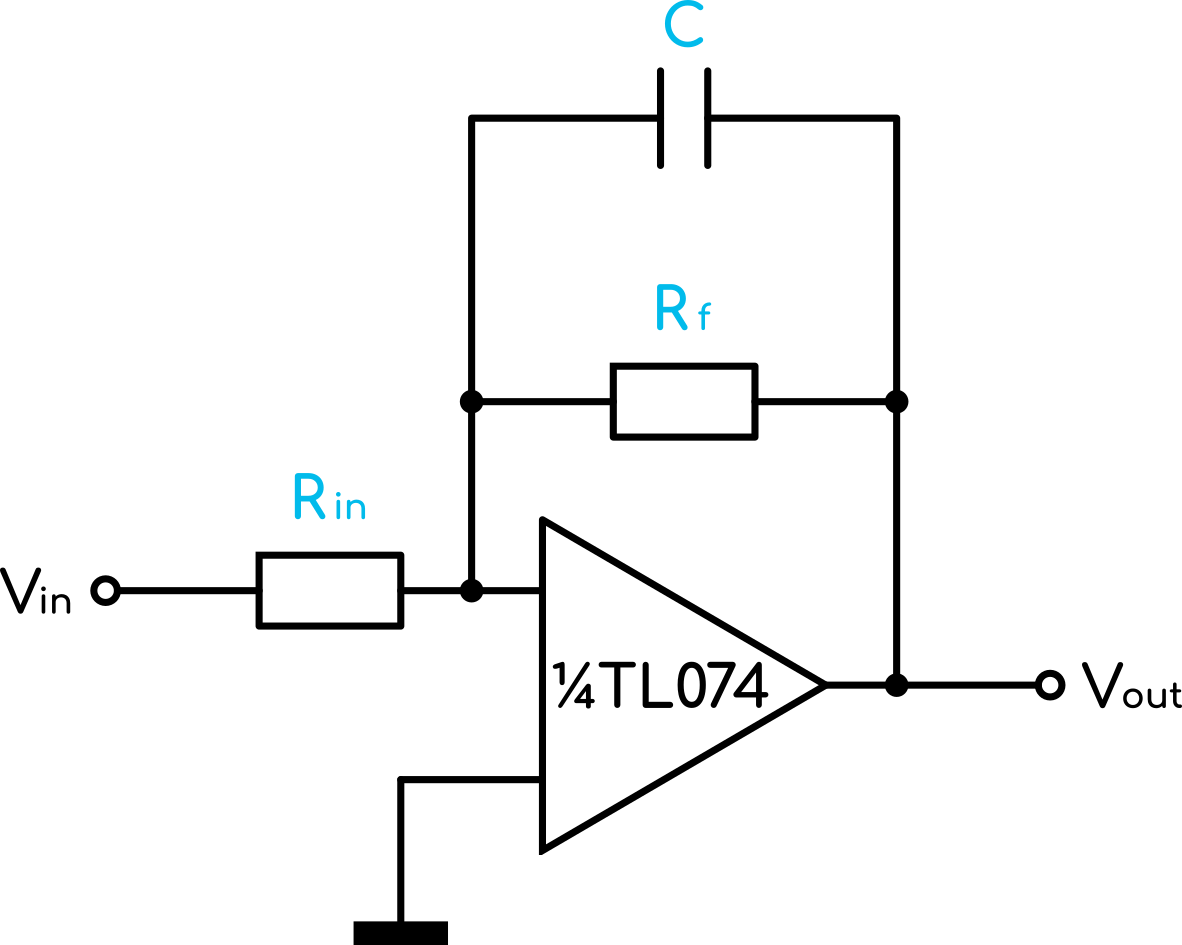
\includegraphics{circuits/active_filter_circuit.png}
    \caption{Circuito del filtro attivo utilizzato}
    \label{active_filter_circuit}
\end{figure}

sfruttando questa soluzione circuitale infatti, tutta la corrente prelevata dal circuito in
uscita verrà fornita dagli amplificatori operazionali. Le relazioni del circuito sono le
seguenti:

\begin{equation}\label{active_filter}
    V_{out}=-V_{in}\frac{R_f}{R_{in}}\cdot\frac{1}{1+j\omega R_fC}\ [V]
\end{equation}

\begin{equation}\label{fcut}
    f_{cut}=\frac{1}{2\pi R_fC}\ [Hz]
\end{equation}

\begin{equation}\label{gain1}
    A_{dB}=20log_{10}\left(\left|\frac{R_f}{R_{in}}\cdot\frac{1}{1+j\omega R_fC}\right|\right)\ [dB]
\end{equation}

oppure, dai valori misurati:

\begin{equation}\label{gain2}
    A_{dB}=20log_{10}\left(\frac{V_{rms\_out}}{V_{rms\_in}}\right)\ [dB]
\end{equation}

La frequenza di taglio viene presa attorno ai $50\ kHz$ per conservare tutto lo spettro audio
e rimuovere invece disturbi in alta frequenza dovuti ad esempio ai segnali di clock.
Scegliendo $R_f=100\ k\Omega$ quindi, il valore del condensatore va preso di circa $30\ pF$,
mentre $R_{in}$ deve avere valore pari a $R_f$. In questo modo si ottiene guadagno unitario e

\begin{equation}
    f_{cut}=\frac{1}{2\pi\cdot100\cdot10^3\cdot30\cdot10^-12}\approx53\ kHz
\end{equation}

Il setup di misura viene riportato in figura \ref{mis_filter}. Per la verifica del funzionamento
si misura il $V_{rms}$ di un segnale sinusoidale in ingresso e in uscita al filtro, agendo
sulla frequenza del suddetto segnale.

\begin{figure}[H]
    \centering
    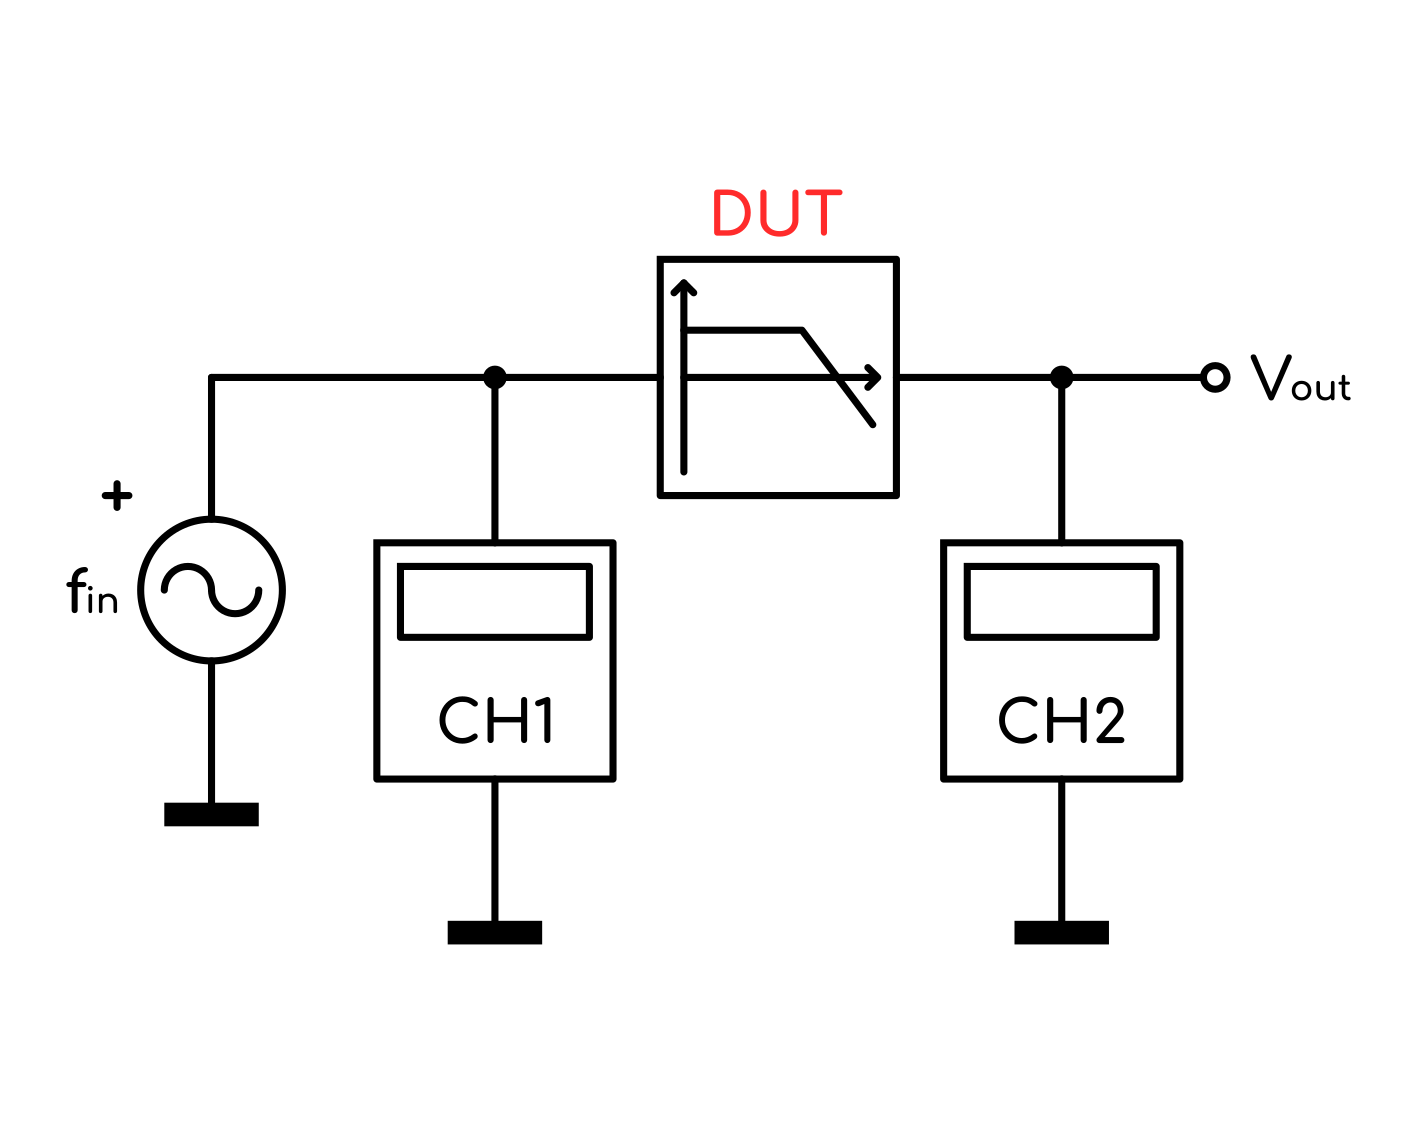
\includegraphics{block_diagrams/mis_filter.png}
    \caption{Setup di misura}
    \label{mis_filter}
\end{figure}

Successivamente, con la formula \ref{gain2} si calcola il valore del guadagno. Infine i dati
vengono raccolti in tabella, riportati in grafico e confrontati con i valori teorici calcolati
con la formula \ref{gain1}.

\begin{table}[H]
    \centering
    \csvreader[
    tabular = |C|C||C|L|,
    table head = {\hline \rowcolor{myLightGrey} $f_{in}\ [kHz]$ & $V_{rmsin}\ [V]$ & $V_{rmsout}\ [V]$ & $A_{dB}\ [dB]$\\\hline},
    late after line = \\\hline,
    ]{data/misure_bode.csv}{}{
    \csvcoli & \csvcolii & \csvcoliii & \csvcolv
    }
    \caption{Misure del guadagno del filtro attivo}
    \label{filter_table}
\end{table}

\begin{figure}[H]
    \centering
    \begin{tikzpicture}
        \centering
        \begin{semilogxaxis}[
                title = Diagramma di bode del filtro,
                no marks,
                width = 0.95\textwidth,
                height = 0.45\textwidth,
                xmin = 0.1, xmax = 4000,
                ymin = -40, ymax = 5,
                grid = major,
                grid style = {dashed, gray!30},
                xlabel = $f_{in}$,
                ylabel = $A_{dB}$,
                x unit = \si{\kHz}, y unit = \si{\dB},
                legend style = {at = {(0.5, -0.25)}, anchor = north},
                cycle list name = modular,
            ]

            \addplot
            table[x = fin, y = A dB calcolato, col sep = comma]{./data/misure_bode.csv};

            \addplot
            table[x = fin, y = A dB misurato, col sep = comma]{./data/misure_bode.csv};

            \legend{Formula \ref{gain1}, Formula \ref{gain2} (con i valori misurati)}
        \end{semilogxaxis}
    \end{tikzpicture}
\end{figure}

\begin{figure}[H]
    \centering

    \begin{subfigure}{.5\textwidth}
        \centering
        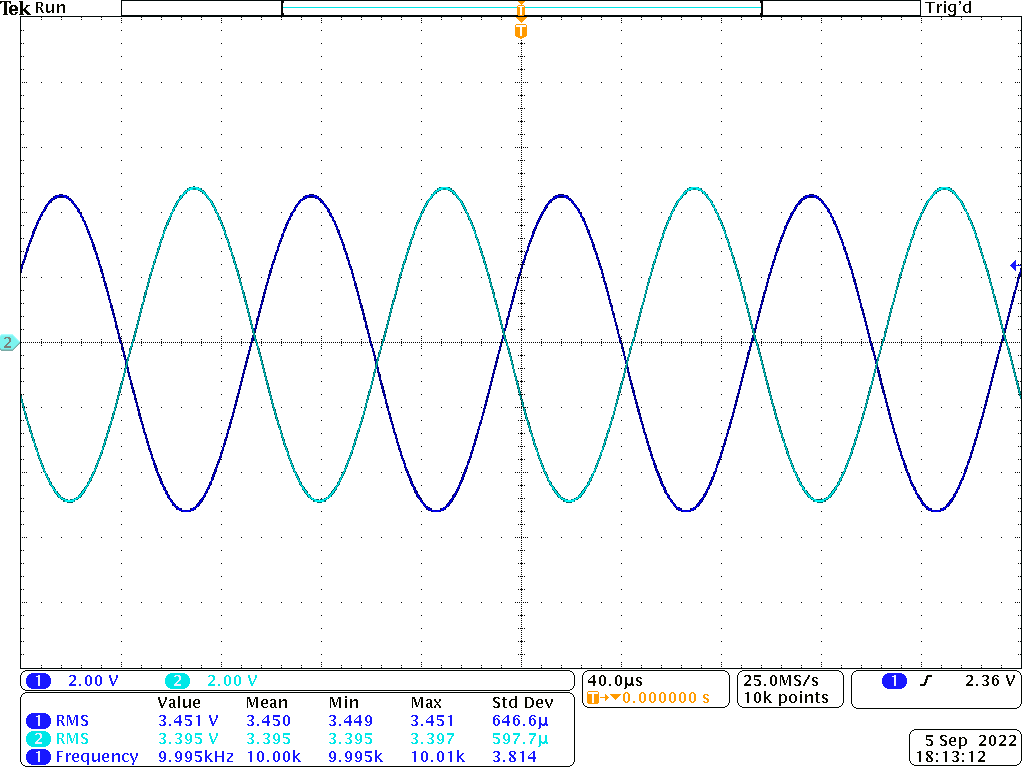
\includegraphics[scale = 0.2]{acquisitions/filter_10kHz.png}
        \caption{$f_{in}=10\ kHz$}
        \label{acq_filter_10kHz}
    \end{subfigure}%
    \begin{subfigure}{.5\textwidth}
        \centering
        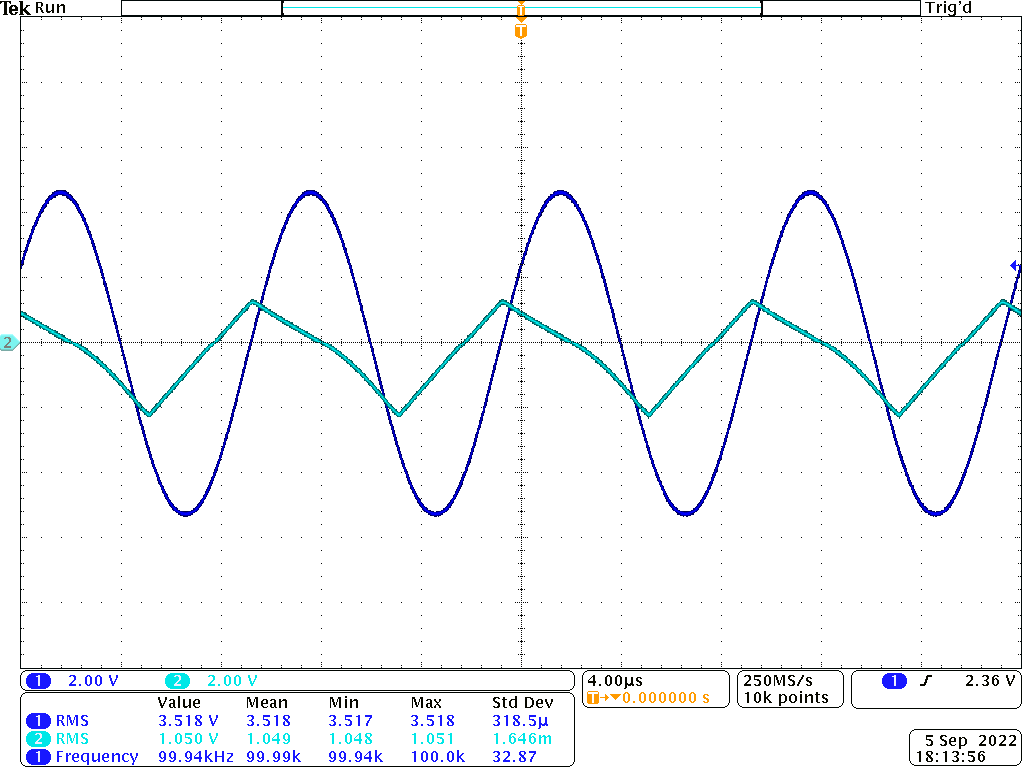
\includegraphics[scale = 0.2]{acquisitions/filter_100kHz.png}
        \caption{$f_{in}=100\ kHz$}
        \label{acq_filter_100kHz}
    \end{subfigure}
    \begin{subfigure}{.5\textwidth}
        \centering
        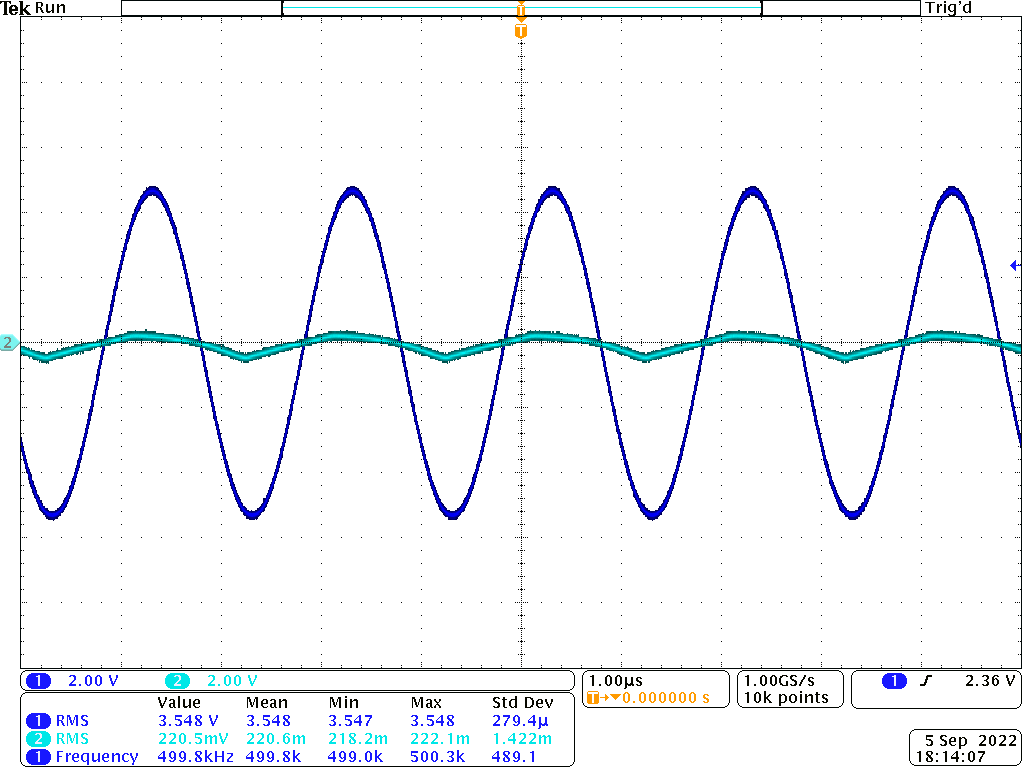
\includegraphics[scale = 0.2]{acquisitions/filter_500kHz.png}
        \caption{$f_{in}=500\ kHz$}
        \label{acq_filter_500kHz}
    \end{subfigure}%
    \begin{subfigure}{.5\textwidth}
        \centering
        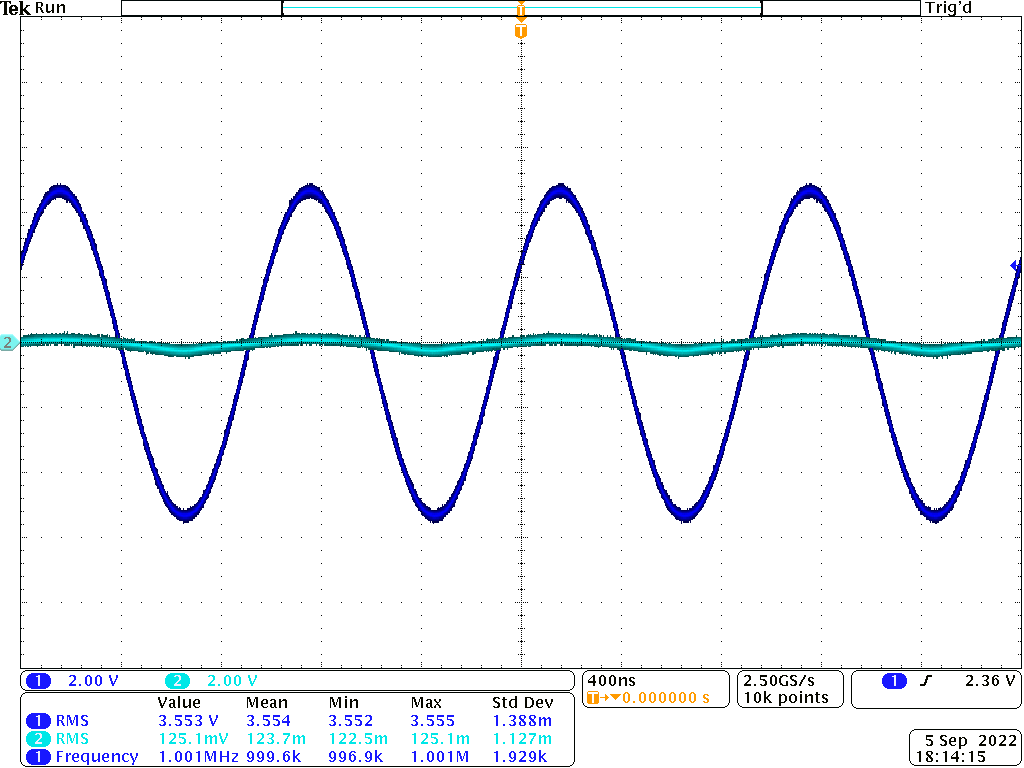
\includegraphics[scale = 0.2]{acquisitions/filter_1MHz.png}
        \caption{$f_{in}=1\ MHz$}
        \label{acq_filter_MHz}
    \end{subfigure}

    \caption{Acquisizioni dei segnali in ingresso e uscita al filtro per diversi valori di $f_{in}$}
    \label{acq_filter}
\end{figure}

In serie ai filtri per le onde a rampa e dente di sega viene anche collegato un amplificatore
invertente con guadagno unitario, con schema uguale a quello rappresentato in figura \ref{inverting_amp_circuit}
per riportare le onde alla loro forma originale, in quanto non sono simmetriche, come lo sono
invece le altre 3.

Infine, in serie a tutte le uscite degli ultimi operazionali prima del connettore, si collegano
delle resistenze di protezione, dal valore di circa $1\ k\Omega$ per limitare la corrente in
uscita in caso di eventuali cortocircuiti, che potrebbero provocare danni agli amplificatori
operazionali, e in ingresso i segnali vengono collegati ad un potenziometro per la regolazione
del volume in uscita.

\begin{figure}[H]
    \centering

    \begin{subfigure}{\textwidth}
        \centering
        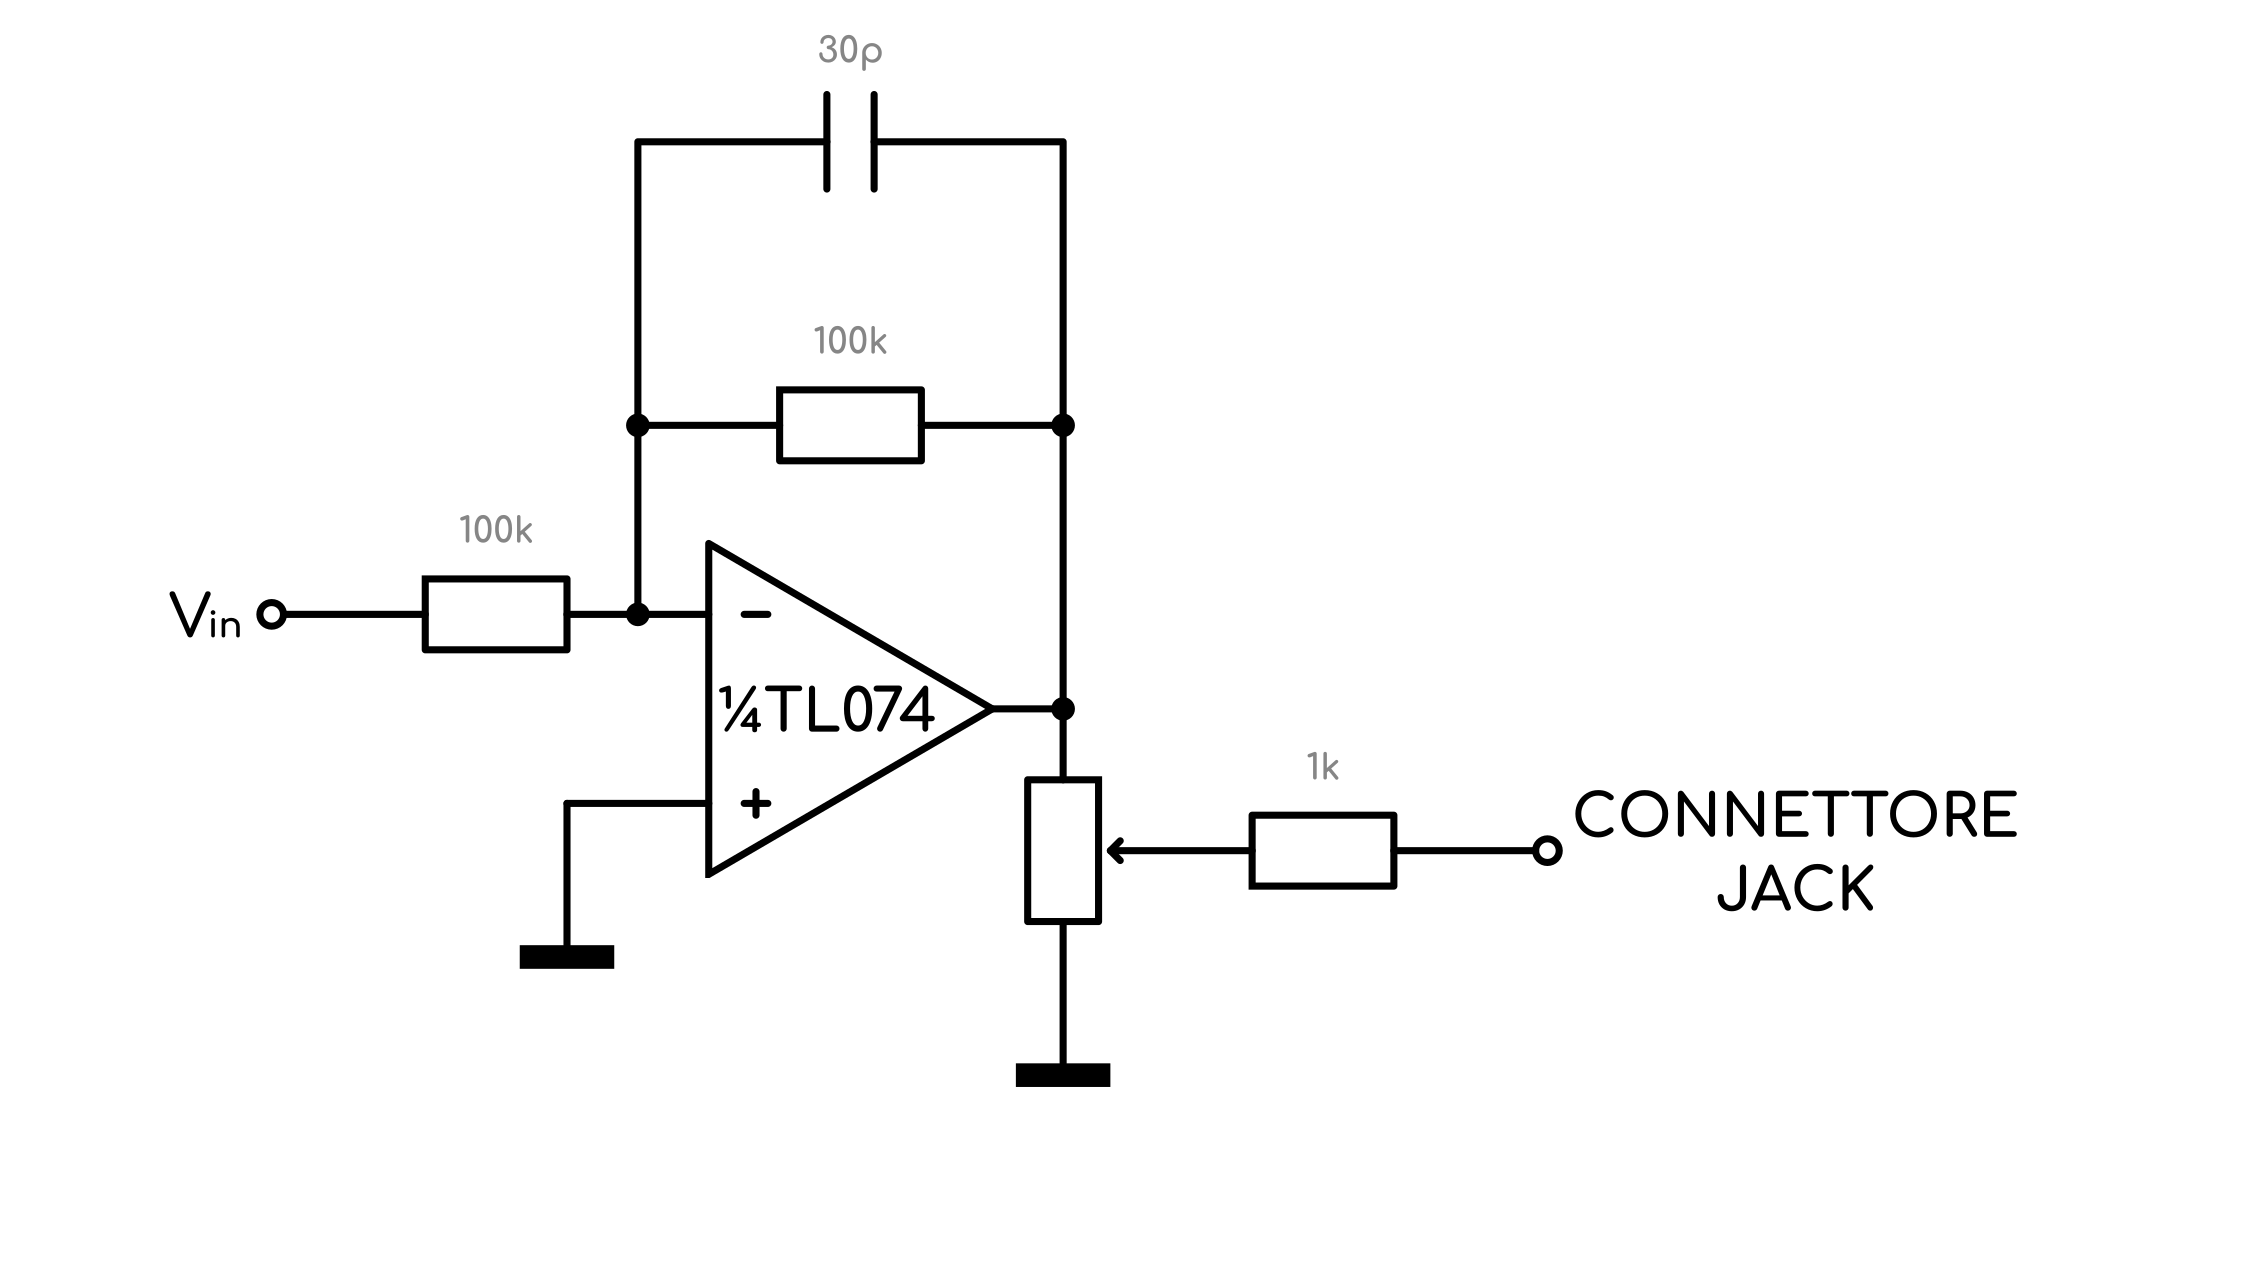
\includegraphics{circuits/inverting_output_stage_circuit.png}
        \caption{Circuito utilizzato per triangolo, sinusoide e onda quadra}
        \label{inverting_output_stage_circuit}
    \end{subfigure}
    \begin{subfigure}{\textwidth}
        \centering
        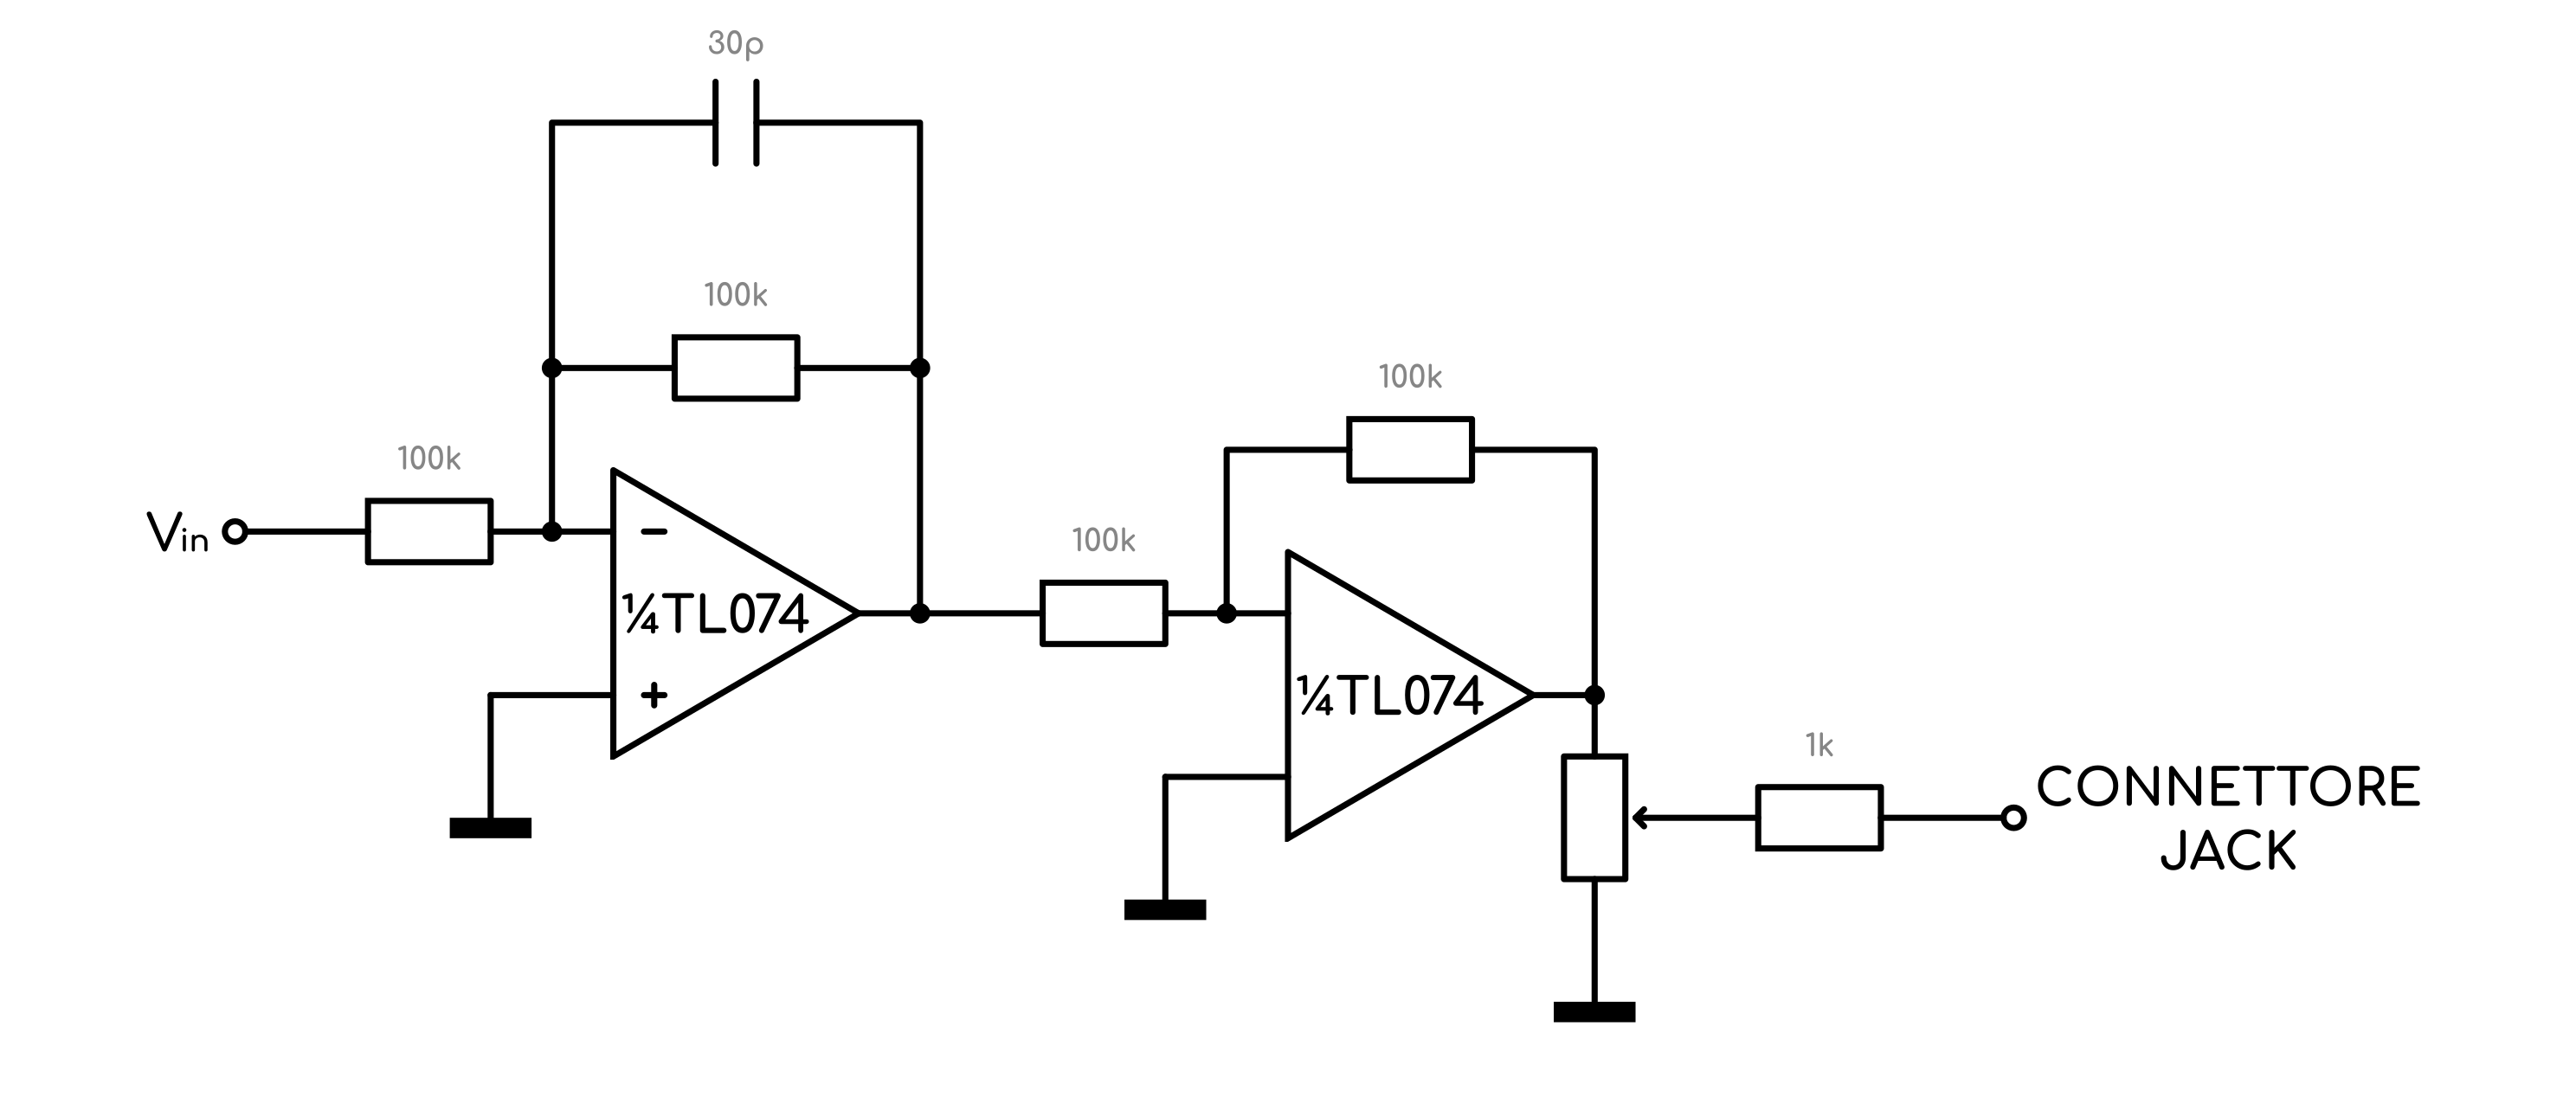
\includegraphics{circuits/noninverting_output_stage_circuit.png}
        \caption{Circuito utilizzato per rampa e dente di sega}
        \label{noninverting_output_stage_circuit}
    \end{subfigure}

    \caption{Stadi d'uscita completi}
    \label{output_stages}
\end{figure}

%--------------------------------------------------------------------------------------------

%\chapter{Protezione del Circuito}

TODO
\unchapter{Conclusioni}

%--------------------------------------------------------------------------------------------

\unsection{Suddivisione delle Schede}

%--------------------------------------------------------------------------------------------

Ogni blocco discusso finora viene collegato assieme secondo il seguente schema:

\begin{figure}[H]
    \centering
    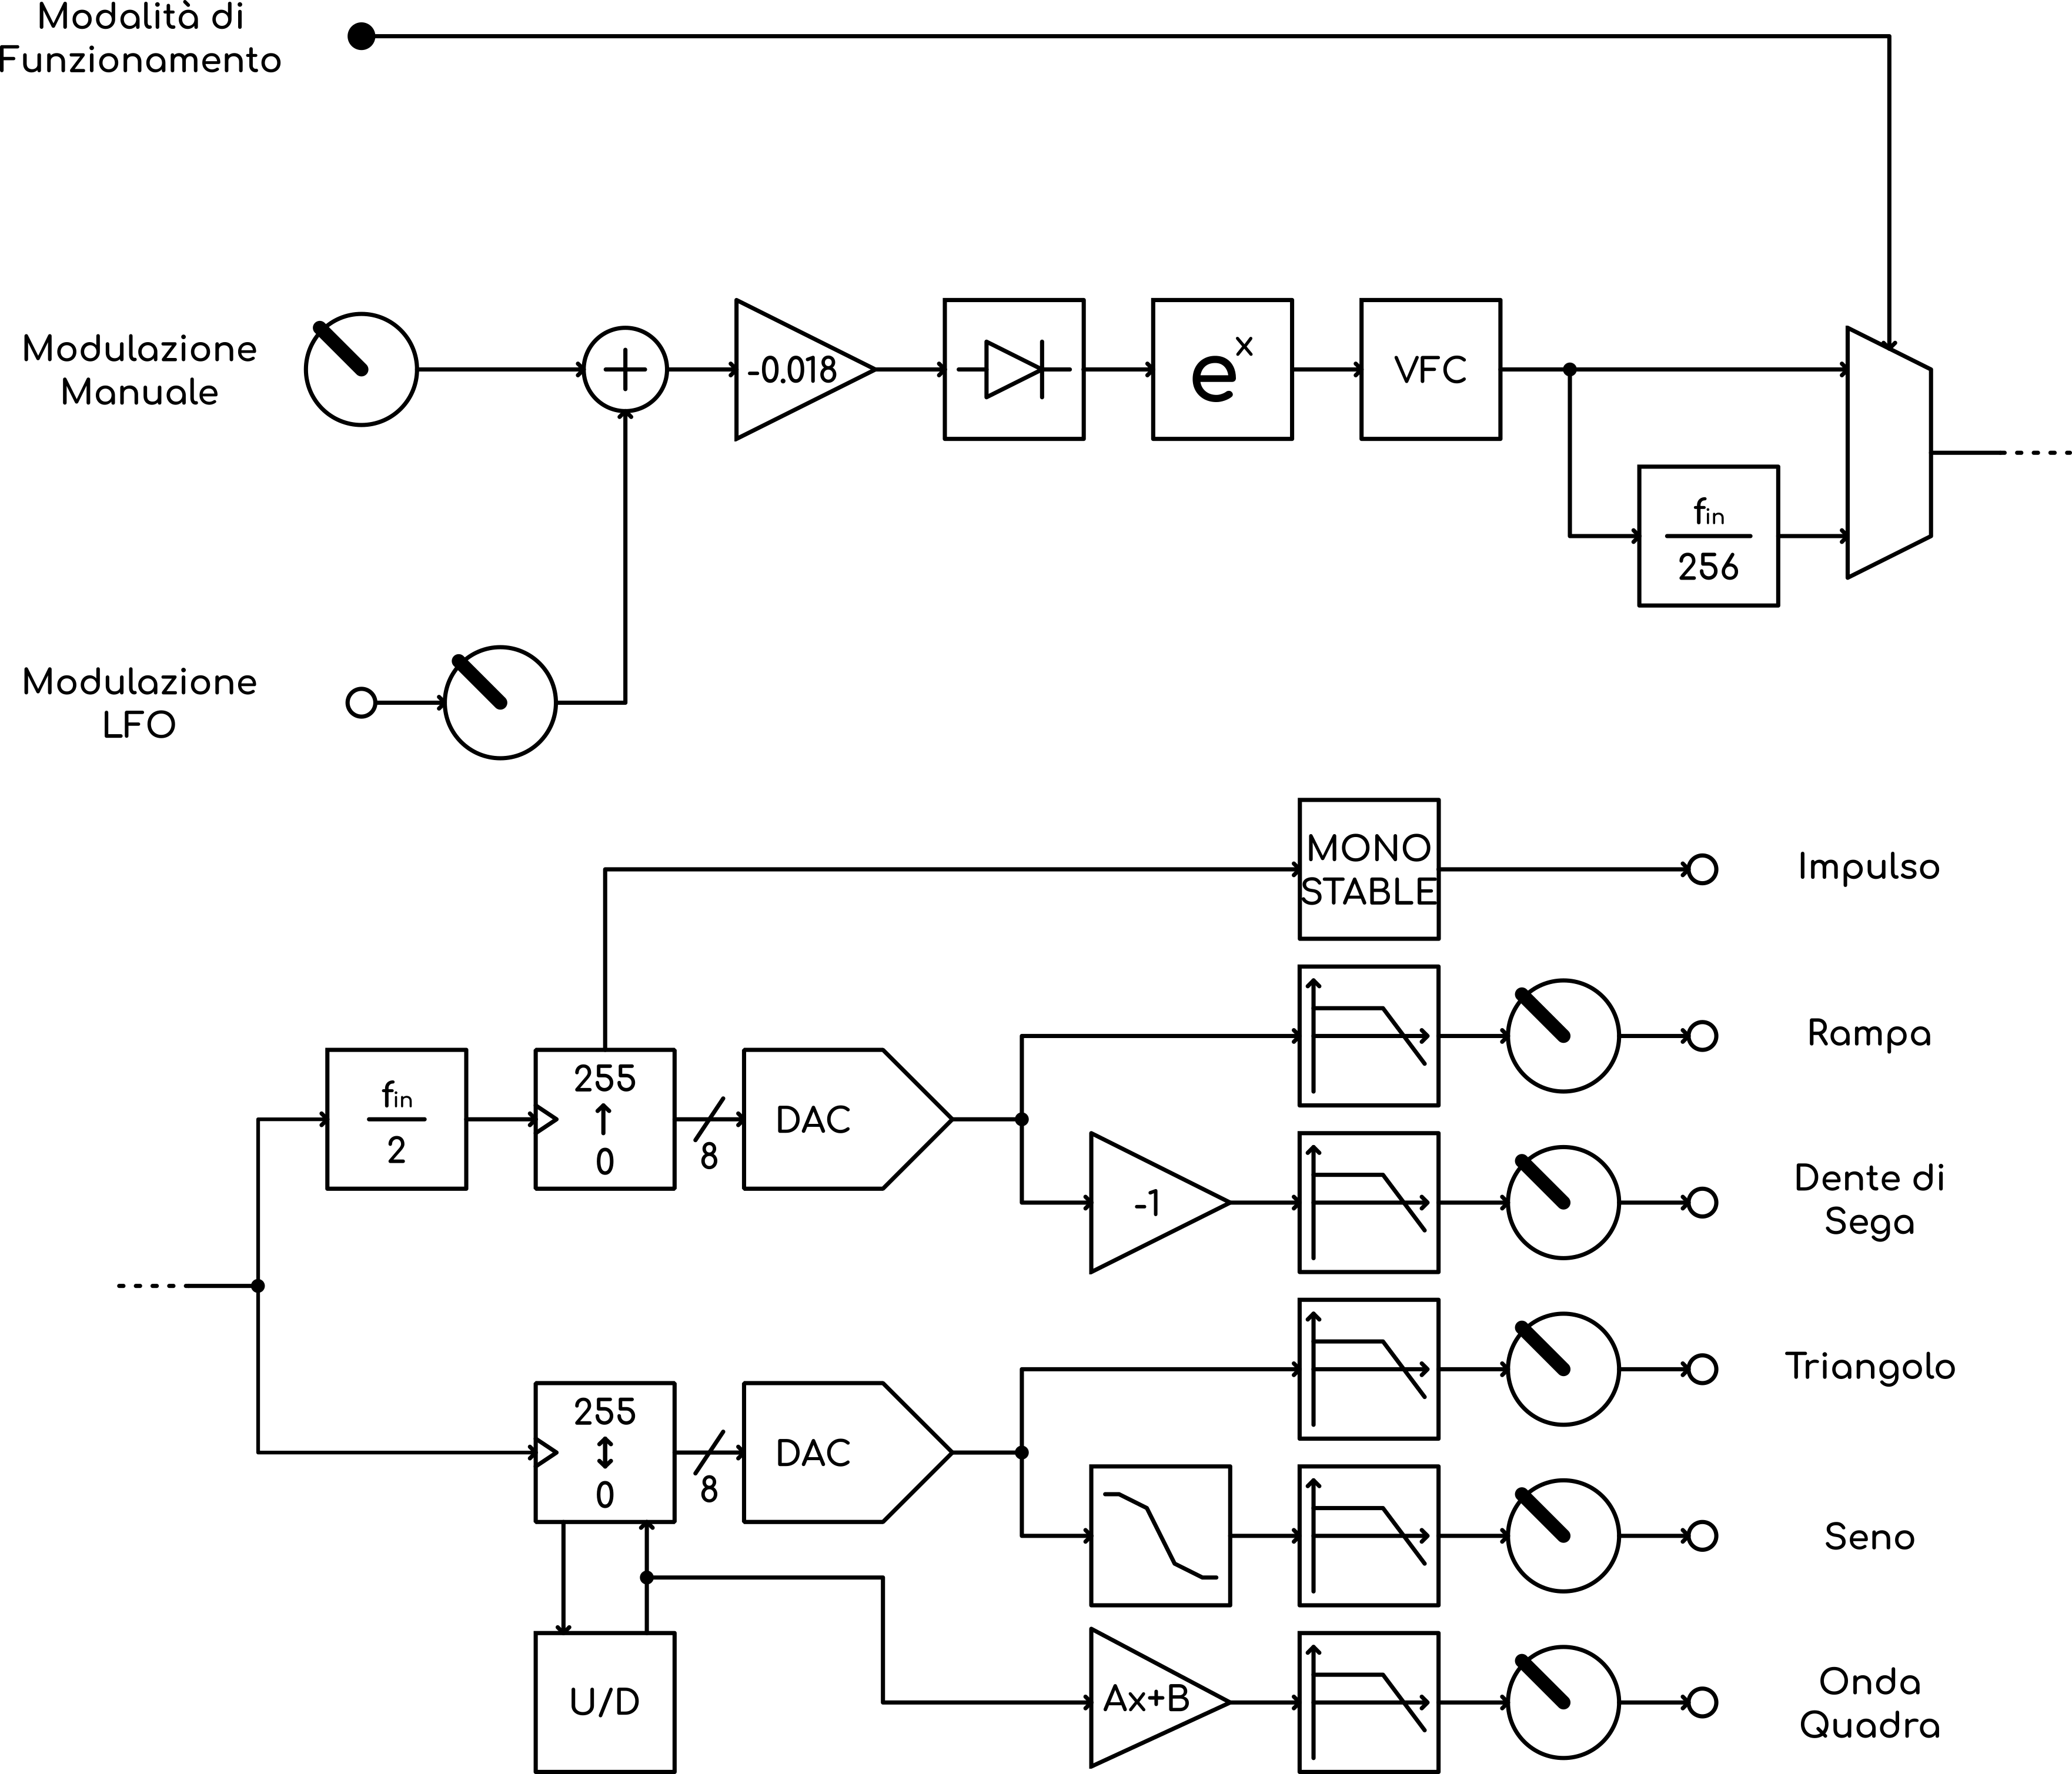
\includegraphics[scale = 0.5]{block_diagrams/full_block_diagram.png}
    \caption{Schema a blocchi completo}
    \label{full_block_diagram}
\end{figure}

Si suddivide poi l'intero circuito in un totale di 3 schede, in modo da ridurre al
minimo l'ingombro del modulo e non avere delle schede troppo dense di componenti.

\begin{figure}[H]
    \centering
    \includegraphics[scale = 0.5]{block_diagrams/full_block_diagram_colored.png}
    \caption{Suddivisione dei blocchi nelle varie schede}
    \label{full_block_diagram_colored}
\end{figure}

Le schede verranno impilate una sopra l'altra e collegate tra loro con degli appositi connettori.
L'interfaccia mostrata in figura \ref{panel_explained} sarà effettivamente il pannello
frontale del nostro modulo, subito sotto andrà la scheda di interfaccia, la quale ospiterà
tutti i componenti atti all'interazione con l'utente e gli altri moduli (manopole, connettori
jack, LED, interruttori, ecc...). Nelle altre due schede invece si collocherà tutto il resto
del circuito secondo quanto specificato in figura.

\begin{figure}[H]
    \centering
    \includegraphics{misc/boards_layout.png}
    \caption{Composizione schede}
    \label{boards_layout}
\end{figure}

Gli schemi elettrici finali utilizzati sono riportati nell'appendice \ref{circuit_diagrams}.

%--------------------------------------------------------------------------------------------

\unsection{Possibili Impieghi del Modulo}

%--------------------------------------------------------------------------------------------

Il modulo in sè non risulta comodamente utilizzabile da solo, e va integrato in un sistema
adeguato assieme a filtri, amplificatori e altri diversi moduli con funzioni varie ed eventuali.
Si riportano allora degli esempi di utilizzo:

\begin{figure}[H]
    \centering
    \includegraphics{block_diagrams/example_setup_1.png}
    \caption{Setup d'esempio 1}
    \label{example_setup_1}
\end{figure}

In questo setup si fa uso di un sequenziatore, in grado di fornire un segnale di controllo
che andrà a determinare la nota generata dall'oscillatore. Successivamente il segnale grezzo
generato dall'oscillatore viene modificato da un filtro controllabile in tensione (Voltage
Controlled Filter, o VCF) e poi fornito ad un sistema per la riproduzione del suono.

\begin{figure}[H]
    \centering
    \includegraphics{block_diagrams/example_setup_2.png}
    \caption{Setup d'esempio 2}
    \label{example_setup_2}
\end{figure}

Qui invece, la nota generata rimane costante nel tempo, ma attraverso una combinazione di un
LFO e un amplificatore controllato in tensione (Voltage Controlled Amplifier, o VCA), si
modifica il volume del suono che viene poi filtrato e riprodotto.

\begin{figure}[H]
    \centering
    \includegraphics{block_diagrams/example_setup_3.png}
    \caption{Setup d'esempio 3}
    \label{example_setup_3}
\end{figure}

In questo ultimo esempio infine, il sequenziatore determina la nota generata dal VCO e la
frequenza di taglio del filtro. Inoltre la sua uscita gate viene data in pasto ad un generatore
di inviluppo, che si occupa di creare un particolare segnale composto da 4 fasi, ovvero attacco,
discesa, sostegno e rilascio, che viene poi utilizzato per il controllo del volume della nota.
Ancora una volta il segnale viene filtrato e poi riprodotto tramite un adeguato sistema.

%--------------------------------------------------------------------------------------------

\unsection{Considerazioni Finali}

%--------------------------------------------------------------------------------------------

Come già accennato nell'introduzione, la progettazione del modulo sarebbe stata largamente
semplificata se si fossero utilizzati dei microcontrollori, tuttavia l'implementazione
analogica realizzata risulta comunque ottima per lo scopo. È ad ogni modo possibile la
progettazione di una scheda con microcontrollori che realizza le stesse funzioni delle schede
discusse in questa tesi, e che può quindi essere eventualmente sostituita al corrispettivo
analogico, sfruttando la divisione delle schede scelta.

\begin{figure}[H]
    \centering
    \includegraphics{misc/boards_layout_microcontroller.png}
    \caption{Composizione schede con scheda a microcontrollore}
    \label{boards_layout_microcontroller}
\end{figure}

Per quanto riguarda l'obiettivo, possiamo dire che le specifiche di progetto fornite al
capitolo \ref{introduzione} sono state pienamente rispettate a meno della precisione sulle
note prodotte che risultano in un range leggermente diverso da quello desiderato.

% tabella frequenze per valori di tensione

Tuttavia un aspetto che meriterebbe più attenzioni è l'effetto della temperatura dell'ambiente
sul convertitore lineare-esponenziale, in quanto effettivamente $V_T$ è funzione di essa.
Tale problema potrebbe essere risolto con l'impiego di una termoresistenza adeguatamente
dimensionata, ma non si scenderà oltre in dettaglio.

%--------------------------------------------------------------------------------------------

\newpage
\unsection{Risultato}

%--------------------------------------------------------------------------------------------

Per concludere si riportano delle foto del risultato finale ottenuto.

\begin{figure}[H]
    \centering

    \begin{subfigure}{.5\textwidth}
        \centering
        \includegraphics[height = \textwidth]{misc/module_result.jpeg}
        \caption{Modulo realizzato}
        \label{module_result}
    \end{subfigure}%
    \begin{subfigure}{.5\textwidth}
        \centering
        \includegraphics[height = \textwidth]{misc/module_result_side.jpeg}
        \caption{Vista lato}
        \label{module_result_side}
    \end{subfigure}

    \caption*{}
\end{figure}

(foto da sistemare)

%--------------------------------------------------------------------------------------------


% appendice schemi elettrici
% schemi elettrici
\appendix
\chapter{Schemi Elettrici delle Schede}\label{circuit_diagrams}

Si riportano gli schemi elettrici disegnati su CAD per il progetto delle schede stampate.

\includepdf[
    width = \textwidth,
    pagecommand = {\thispagestyle{plain}},
    pages = -,
    nup = 1x2,
    offset = 5mm 0mm
]{
    pdfs/schematics/FG-VCO-(complete).pdf
}

% bibliografia
\printbibliography
\addcontentsline{toc}{chapter}{Bibliografia}

% fine del documento
\end{document}